% !TEX root = ../main.tex
\renewcommand{\localPath}{chap2}

\chapter{Modèle hybride linéarisé dans le cas $1dx-1dv$}

%\newcommand{\commentaire}[2][]{\ifthenelse{\equal{#1}{}}{\textbf{#2}}{\ifthenelse{\equal{#1}{Anais}}{\textcolor{magenta}{#2}}{\ifthenelse{\equal{#1}{Nicolas}}{\textcolor{orange}{#2}}{\textcolor{teal}{#2}\footnote{Commentaire rédigé par #1}}}}}

%% section 1
% !TEX root = ../chap3.tex

\section{Introduction}

L'objectif de ce chapitre est d'étendre les stratégies développées pour la résolution d'un modèle hybride linéarisé, présentées dans le chapitre~\ref{chap2}, au cas $1dz-3dv$ permettant de prendre en compte, entre autre, les effets du champ magnétique sur la dynamtique des particules. Nous étudierons dans ce chapitre un modèle hybride, ce qui suppose que la distribution de particules est composée de deux populations, une première ayant une vitesse thermique faible, et considérée comme \emph{froide}, dont on approximera la dynamique comme celle d'un fluide ; une seconde population ayant une vitesse thermique plus élevée, considérée comme \emph{chaude}, mais contrairement au chapitre~\ref{chap2}, celle-ci n'a pas besoin d'être distribuée selon une bi-maxwellienne. Ce type de modèle peut être utilisé pour modéliser des particules d'un plasma dans un tokamak, ou des particules du vent solaire interagissant avec la magnétosphère terrestre. Dans ces contextes les particules se déplacent de manière hélicoïdale selon les lignes du champ extérieur $\vb{B}_0 = (0,0,B_0)^\top$, et seul le déplacement dans cette direction sera étudié ici, ce qui explique le nom de la seule variable d'espace considérée : $z$. Pour le déplacement hélicoïdale complet \Josselin{il faudrait ajouter ici une référence que je n'ai pas car je ne connais pas trop ces modèles, de mémoire c'est ce que faisait Xiaofei}.

La prise en compte des effets du champ magnétique dans le modèle nous mène à considérer un système à 7 inconnues $(j_{c,x},j_{c,y},B_x,B_y,E_x,E_y,f_h)$, ce qui induit un coût de calcul bien plus important avec les méthodes eulériennes que nous étudions. Pour diminuer ce coût de calcul nous souhaitons diminuer le nombre d'itérations tout en assurant la stabilité des méthodes considérées ; cela se fait en augmentant le pas de temps $\Delta t$ et en estimant les contraintes de stabilité. L'utilisation de méthodes d'ordre élevés en temps, en espace et en vitesse, permet de réduire l'erreur, capturer la dynamique non-linéaire du système, avec peu de points de discrétisation.

Nous souhaitons dans ce chapitre comparer deux méthodes d'ordre élevé en temps et dans l'espace des phrases, sur un cas à 4 dimensions, plus proches d'applications physiques, il s'agit d'une généralisation des deux stratégies développées dans le chapitre~\ref{chap2}, une méthode de \emph{splitting} et une méthode de Lawson. La contrainte du nombre de dimensions ne permet pas de raffiner le maillage\footnote{Pour une discrétisation de $128$ points par direction, la grille contient $128^4$ points, soit, représentées avec des réels à virgule flottante à double précision (64 bits), un espace mémoire de 2Go pour la seule variable $f_h$ ; une méthode de Lawson d'ordre 4 nécessite la sauvegarde des étages intermédiaires, donc $4\times 2\textrm{Go}$ minimum. L'utilisation de transformées de Fourier impose de travailler avec des nombres complexes, ce qui nécessite de doubler l'utilisation mémoire pour la même précision.}, ce qui ne permet pas l'accès à une solution de référence, nous devrons nous contenter de regarder les invariants (comme l'énergie totale), et de comparer les résultats aux taux d'instabilités fournis par les relations de dispersion.

Pour résoudre les problèmes que pose ce problème nous présenterons tout d'abord le modèle hybride $1dz-3dv$, puis nous détaillerons les schémas numériques que nous considérons. La méthode de \emph{splitting} hamiltonien contient 7 étapes, rendant de fait l'ordre élevé (méthode de Suzuki) trop coûteux pour approfondir son étude, nous nous concentrerons donc sur des méthodes de \emph{splitting} d'ordre plus faible. Pour la méthode de Lawson, il est envisageable d'effectuer un filtrage du terme induit pas le champ magnétique externe $\vb{B}_0$, permettant d'augmenter le pas de temps stabilisant la méthode. La partie linéaire du système introduit une matrice dont il n'est pas possible de calculer exactement son exponentielle, pourtant nécessaire pour la mise en œuvre d'une méthode de Lawson perforante. Nous étudierons un premier cas où nous ne profitons pas pleinement de toute la partie linéaire du système, introduisant ainsi une condition de stabilité ; puis nous proposerons une méthode permettant, à l'aide de méthodes approchées comme la troncature de la série de Taylor ou les approximants de Padé, de calculer une approximation de l'exponentielle de toute la partie linéaire, permettant ainsi de se soustraire à une condition de stabilité. \Josselin{Mettre les références vers les sections.}

%% section 2
% !TEX root = ../chap3.tex

\section{Présentation du modèle}

\begin{align}
  \label{eq:VHM:jx}
  &\pdv{j_{c,x}}{t} = \Omega_{pe}^2 { E}_x - { j}_{c,y}B_0,\\
  \label{eq:VHM:jy}
  &\pdv{j_{c,y}}{t} = \Omega_{pe}^2 { E}_y + { j}_{c,x}B_0,\\
  \label{eq:VHM:Bx}
  &\pdv{B_{x  }}{t} = \partial_z E_y,\\
  \label{eq:VHM:By}
  &\pdv{B_{y  }}{t} = -\partial_z E_x,\\
  \label{eq:VHM:Ex}
  &\pdv{E_{x  }}{t} =-\partial_z B_y - {j}_{c,x} + \int v_x f_h \dd{\vb{v}},\\
  \label{eq:VHM:Ey}
  &\pdv{E_{y  }}{t} =\partial_z B_x - {j}_{c,y} + \int v_y f_h \dd{\vb{v}}, \\
  \label{eq:VHM:fh}
  &\pdv{f_{h  }}{t} +  v_z\partial_z f_h - \left(E_x + v_y B_0 - v_zB_y\right)\partial_{v_x} f_h\\
  &\hspace{2cm}- \left(E_y - v_x B_0 + v_z B_x\right)\partial_{v_y} f_h- \left(v_x B_y- v_y B_x\right)\partial_{v_z} f_h = 0.\nonumber
\end{align}
Cela nous permet de définir l'hamiltonien :
\begin{equation}
  \mathcal{H} = {}
      \underbrace{\frac{1}{2}\int_{\mathbb{R}}(E_x^2+E_y^2) \dd{z}}_{\mathcal{H}_E}
    + \underbrace{\frac{1}{2}\int_{\mathbb{R}}(B_x^2+B_y^2) \dd{z}}_{\mathcal{H}_B}
    + \underbrace{\frac{1}{2}\int_{\mathbb{R}}\frac{1}{\Omega_{pe}^2}(j_{c,x}^2+j_{c,y}^2) \dd{z}}_{\mathcal{H}_{j_c}}
    + \underbrace{\frac{1}{2}\int_{\mathbb{R}}\int_{\mathbb{R}^2}|\vb{v}|^2 f_h \dd{\vb{v}}\dd{z}}_{\mathcal{H}_{f_h}}
  \label{eq:ham1dz3dv}
\end{equation}

On définit le crouchet suivant, définit pour deux fonctionnelles $\mathcal{F}$ et $\mathcal{G}$ :
\begin{equation}
  \begin{aligned}
    \{ \mathcal{F},\mathcal{G} \}[ j_{c,x}, j_{c,y}, B_x, B_y, E_x, E_y, f_h] &=
                       \int_{\mathbb{R}}\int_{\mathbb{R}^3} f_h \left( \partial_z\fdv{\mathcal{F}}{f_h}\partial_{v_z}\fdv{\mathcal{G}}{f_h} - \partial_{v_z}\fdv{\mathcal{F}}{f_h}\partial_z\fdv{\mathcal{G}}{f_h} \right) \dd{\vb{v}}\dd{z} \\
      &\hspace{-4cm} + \int_{\mathbb{R}}\int_{\mathbb{R}^3} f_h \left(
            \partial_{v_x}\fdv{\mathcal{F}}{f_h}\fdv{\mathcal{G}}{E_x} + \partial_{v_y}\fdv{\mathcal{F}}{f_h}\fdv{\mathcal{G}}{E_y}
          - \partial_{v_x}\fdv{\mathcal{G}}{f_h}\fdv{\mathcal{F}}{E_x} - \partial_{v_y}\fdv{\mathcal{G}}{f_h}\fdv{\mathcal{F}}{E_y}
          \right) \dd{\vb{v}}\dd{z} \\
      &\hspace{-4cm} + \int_{\mathbb{R}}\int_{\mathbb{R}^3} f_h(\vb{B}+\vb{B}_0)\cdot\left( \nabla_{\vb{v}}\fdv{\mathcal{F}}{f_h}\times\nabla_{\vb{v}}\fdv{\mathcal{G}}{f_h} \right) \dd{\vb{v}}\dd{z} \\
      &\hspace{-4cm} + \int_{\mathbb{R}} \left(
          - \partial_z\fdv{\mathcal{F}}{E_y}\fdv{\mathcal{G}}{B_x} + \partial_z\fdv{\mathcal{F}}{E_x}\fdv{\mathcal{G}}{B_y}
          + \partial_z\fdv{\mathcal{G}}{E_y}\fdv{\mathcal{F}}{B_x} - \partial_z\fdv{\mathcal{G}}{E_x}\fdv{\mathcal{F}}{B_y}
          \right) \dd{z} \\
      &\hspace{-4cm} + \int_{\mathbb{R}} \Omega_{pe}^2 \left(
            \fdv{\mathcal{F}}{j_{c,x}}\fdv{\mathcal{G}}{E_x} + \fdv{\mathcal{F}}{j_{c,y}}\fdv{\mathcal{G}}{E_y}
          - \fdv{\mathcal{G}}{j_{c,x}}\fdv{\mathcal{F}}{E_x} - \fdv{\mathcal{G}}{j_{c,y}}\fdv{\mathcal{F}}{E_y}
          \right) \dd{z} \\
      &\hspace{-4cm} + \int_{\mathbb{R}} \Omega_{pe}^2B_0 \left(
            \fdv{\mathcal{F}}{j_{c,x}}\fdv{\mathcal{G}}{j_{c,y}}
          - \fdv{\mathcal{F}}{j_{c,y}}\fdv{\mathcal{G}}{j_{c,x}}
          \right) \dd{z}.
  \end{aligned}
  \label{bracket}
\end{equation}
Cela nous permet de réécrire le système~\eqref{eq:VHM:jx}-\eqref{eq:VHM:fh} comme 
$$
  \partial_t U = \{ U,\mathcal{H} \}
$$
où $U(t,z,\vb{v}) = ( j_{c,\perp}(t,z) , B_\perp(t,z) , E_\perp(t,z) , f)h(t,z,\vb{v}) )^\top$ où $\mathcal{H}$ est donné par~\eqref{eq:ham1dz3dv} et $j_{c,\perp}=(j_{c,x},j_{c,y})^\top$, $B_{\perp}=(B_{x},B_{y})^\top$ et $E_{\perp}=(E_{x},E_{y})^\top$. Par la suite, nous utiliserons également les notations $v_\perp = (v_x,v_y)^\top\in\mathbb{R}^2$ ainsi que $\vb{v} = (v_\perp,v_z)^\top\in\mathbb{R}^3$ et nous définissions la matrice symplectique 
$$
  J = \begin{pmatrix}
     0 & 1 \\
    -1 & 0
  \end{pmatrix}.
$$

%% section 3
% !TEX root = ../chap2.tex

\section{Structure géométrique du mod\`ele hybride lin\'earis\'e VHL}
\label{s:geom}

Dans cette partie, nous présentons la structure du modèle hybride linéarisé VHL \eqref{eq:vahl}, à savoir son Hamiltonien et son crochet de Poisson. Pour simplifier les notations, nous notons dans cette section $f=f_h$, $\rho_c=\rho_c^{(0)}$ et $u=u_c$. Cette structure permet notamment d'assurer la préservation de nombreux invariants (énergie totale et opérateurs de Casimir entre autres) mais sera à la base d'un \emph{splitting} en temps, dans l'esprit de \cite{Crouseilles:2015}, \cite{Casas:2017}, \cite{Kraus:2017} \cite{Li:2020}. Nous aurons besoin d'introduire certaines notations pour pouvoir introduire la structure.

Tout d'abord, rappelons que pour une fonctionnelle donnée ${\cal G}(f)$, la dérivée de Fréchet de la distribution $\frac{\delta {\cal G}}{\delta f}(f)$ évaluée au point $f$, est définie par 
\begin{equation}
  {\cal G}(f + \delta f) - {\cal G}(f) = \int_{\Omega\times \mathbb{R}} \frac{\delta {\cal G}}{\delta f}(f)(x, v) \delta f(x, v) \mathrm{d}x\mathrm{d}v +{\cal O}(\delta f^2), 
\end{equation}
pour toute variation régulière $\delta f$. On définit le Hamiltonien associé au modèle VHL \eqref{eq:vahl} 
\begin{eqnarray}
\label{hamiltonian_red}
  \mathcal{H} &=& \frac{1}{2}\int_{\mathbb{R}} {E}^2 \mathrm{d}{x}  +  \frac{1}{2}\int_{\mathbb{R}} \rho_{c} u^2\mathrm{d}{x} + \frac{1}{2}\int_{\mathbb{R}}\int_{\mathbb{R}} v^2 f\,\mathrm{d}x\,\mathrm{d}v, \\
              &=&  \mathcal{H}_E + \mathcal{H}_u + \mathcal{H}_f. 
\end{eqnarray}
Les trois termes correspondent respectivement à l'énergie électrique, l'énergie cinétique des particules froides et l'énergie cinétique des particules chaudes. Pour une fonctionnelle ${\cal G}(E, u, f)$, on notera $\delta {\cal G}/\delta f$, $\delta {\cal G}/\delta E$ et $\delta {\cal G}/\delta u$ les dérivées de Fréchet de ${\cal G}$ par rapport à $f, E$ et $u$ respectivement. On introduit à présent le crochet de Poisson de deux fonctionnelles ${\cal F}(E, u, f)$ et ${\cal G}(E, u, f)$
$$
  \begin{aligned}
    \{ {\cal F}, {\cal G} \}( u, E, f) &= \int_{\mathbb{R}}\int_{\mathbb{R}} f \left( \partial_x \frac{\delta {\cal F}}{\delta f}\partial_{v} \frac{\delta {\cal G}}{\delta f} - \partial_{v} \frac{\delta {\cal F}}{\delta f}\partial_{x} \frac{\delta {\cal G}}{\delta f}\right)\mathrm{d}v \mathrm{d}x \\
                         & + \int_{\mathbb{R}}  \left(  \frac{\delta {\cal F}}{\delta{ u}}  \frac{\delta {\cal G}}{\delta{ E}} - \frac{\delta {\cal F}}{\delta{ E}}  \frac{\delta {\cal G}}{\delta{u}} \right) \mathrm{d}x \\
                         & + \int_{\mathbb{R}}\int_{\mathbb{R}}  \left(  \frac{\delta {\cal F}}{\delta{ E}}  \partial_v f\frac{\delta {\cal G}}{\delta{ f}} - \frac{\delta {\cal G}}{\delta{ E}} \partial_v f \frac{\delta {\cal F}}{\delta{f}} \right) \mathrm{d}{ v}\mathrm{d}x \\
  \end{aligned}
$$
Avec cette notation, le modèle hybride linéarisé~\eqref{eq:vahl} se réécrit alors, avec  $U=(u, E, f)$ et $\mathcal{H}$ donn\'e par \eqref{hamiltonian_red}
\begin{equation}
\label{ham_form}
  \partial_t U = \{ U, \mathcal{H} \}. 
\end{equation}

Dans la suite, on vérifie que la réécriture \eqref{ham_form} est bien équivalente au modèle VHL. 
Pour cela, on a besoin des relations suivantes 
$$
  \frac{\delta \mathcal{H}}{\delta f} = \frac{v^2}{2}, \;\; \frac{\delta \mathcal{H}}{\delta u} = \rho_c u, \;\; \frac{\delta \mathcal{H}}{\delta E} = E. 
$$
De plus, par abus de notation, on notera la fonctionnelle associ\'ee \`a la fonction comme suit (par exemple pour $u$) 
$u(t, z)=\int_{\mathbb{R}} u(t, x)\delta(x-z) \mathrm{d}x$, de sorte que $ \frac{\delta u}{\delta u} = \delta(x-z)$. Pour $f$, 
on notera $f(t, x, w)=\int_{\mathbb{R}} f(t, z, v)\delta(x-z)\delta(w-v) \mathrm{d}x\mathrm{d}v$, de sorte que $ \frac{\delta f}{\delta f} = \delta(x-z)\delta(w-v)$. 

\medskip 

\noindent $\bullet$ On calcule dans un premier temps $\{ u, \mathcal{H} \}$ 
\begin{eqnarray*}
\partial_t u(t, z) = \{ u, \mathcal{H} \} &=& 0+ \int_{\mathbb{R}}   \delta(x-z) E(t,x) \mathrm{d}x  + 0 = E(t,z)
\end{eqnarray*}
\noindent $\bullet$ Puis on considère $\{ E, \mathcal{H} \}$ 
\begin{eqnarray*}
\partial_t E(t, z) = \{ E, \mathcal{H} \} &=& 0 -  \int_{\mathbb{R}}  \delta(x-z) \rho_c u \mathrm{d}x  +  \int_{\mathbb{R}}\int_{\mathbb{R}}  \left(  \delta(x-z)  \partial_v f \frac{v^2}{2}  \right) \mathrm{d}{ v}\mathrm{d}x \nonumber\\
&=& - \rho_c u(t, z) - \int_{\mathbb{R}} f(t, z, v) v\mathrm{d}{ v} 
\end{eqnarray*}
\noindent $\bullet$  Finalement,  $\{ f, \mathcal{H} \}$ donne 
\begin{eqnarray*}
\partial_t f(t, z,w) = \{ f, \mathcal{H} \} &=&  \int_{\mathbb{R}}\int_{\mathbb{R}} f \left( \partial_x (\delta(x-z)\delta(w-v)) \partial_v \frac{v^2}{2}   \right)\mathrm{d}v \mathrm{d}x \nonumber\\
&& + 0  -  \int_{\mathbb{R}}\int_{\mathbb{R}}  \left( E  \partial_v f \right) \delta(x-z)  \delta(w-v)    \mathrm{d}{ v}\mathrm{d}x \nonumber\\
&=& (- v\partial_x f - E\partial_v f)(t, z, w). 
\end{eqnarray*}

Enfin, on peut vérifier  que le crochet de Poisson satisfait les propriétés suivantes 
\begin{itemize}
\item anti-symétrie: $\{ F, G \} = -\{ G, F \}$ 
\item bilinéarité: $\{ F + G, H \} = \{ F, H \}+\{ G, H \}$ 
\item identité de Jacobi : $\{\{ F, G \}, H\} + \{\{G,H\}, F \} + \{\{H, F\}, G \} = 0$.  
\end{itemize}
Les deux premières propriétés sont  simples alors que la dernière est habituellement 
plus compliquée. On utilise les calculs de \cite{Li:2020}, \cite{Morrison:2012}. 

%% section 4
% !TEX root = ../../main.tex

\section{Méthodes de résolution numérique en temps}
%%%%%%%%%%%%%%%%%%%%%%%%%%%%%%%%%%%%%%%%%%%%%%%%%%%%%%%%%%%%%%%%%%%%%%

Dans cette section nous allons présenter les principales méthodes utilisées pour résoudre numériquement des équations dites cinétiques en temps, et plus spécifiquement le système~\eqref{eq:0:vmhl:1}-\eqref{eq:0:vmhl:4}. Une fois discrétisé en $(\vb{x},\vb{v})$, les différents systèmes que nous regardons peuvent se réduire au modèle abstrait suivant :
\begin{equation}
  \dot{u} = L(t,u) + N(t,u),\quad u(0)=u_0
  \label{eq:0:dtu}
\end{equation}
d'inconnue $u\in\mathbb{R}^n$ et où $L$ et $N$ sont des fonctions $(t,u)\in\mathbb{R}_+\times\mathbb{R}^n\mapsto\mathbb{R}^n$, $n\in\mathbb{N}$ est le nombre de dimensions, ou d'inconnues du problème. C'est sur cette équation~\eqref{eq:0:dtu} que nous allons présenter les différentes méthodes d'intégration en temps utilisées ici.

% --------------------------------------------------------------------
\subsection{Méthode de \emph{splitting} hamiltonien}
% --------------------------------------------------------------------

Les méthodes de \emph{splitting} sont classiquement utilisées dans la résolution d'équations cinétiques (\cite{Morrison:2017,Grandgirard:2006,Tronci:2010,Tronci:2014}), elles consistent à diviser l'équation à résoudre en plusieurs parties. La construction de ces méthodes en temps se fait par concaténation des différentes étapes en formant des palindromes.

Une méthode de \emph{splitting} consiste à résoudre les deux équations suivantes successivement :
\begin{eqnarray}
    \dot{u} = L(t,u)\label{eq:0:split:1}\\
    \dot{u} = N(t,u)\label{eq:0:split:2}
\end{eqnarray}
La solution de l'équation~\eqref{eq:0:dtu} au temps $t$ est $\varphi_t(u_0)$, et sera approchée par une composition de $\varphi_t^{[L]}(u_0)$ et $\varphi_t^{[N]}(u_0)$, respectivement solutions de~\eqref{eq:0:split:1} et~\eqref{eq:0:split:2}. Ainsi la méthode de Lie, \emph{splitting} d'ordre 1, consiste à approcher $\varphi_t(u_0)$ par $\varphi_t(u_0)\approx \varphi_t^{[L]} \circ \varphi_t^{[N]}(u_0)$. Si la résolution de chaque sous-système $\varphi_t^{[L]}$ et $\varphi_t^{[N]}$ est exacte, la seule erreur en temps provient du \emph{splitting}.

La résolution de chaque sous-système peut se faire sur des intervalles de temps différents (que nous noterons en indice), ainsi la méthode de Strang~\cite{Strang:1968}, \emph{splitting} d'ordre 2, s'écrit comme :
$$
  u(t) = S_{t}(u_0) = \varphi^{[L]}_{t/2}\circ\varphi^{[N]}_{t}\circ\varphi^{[L]}_{t/2}(u_0)
$$

Lorsque l'équation met en jeu plusieurs termes, comme c'est le cas pour le système~\eqref{eq:0:vmhl:1}-\eqref{eq:0:vmhl:4}, il est difficile de savoir comment choisir $L$ et $N$. L'hamiltonien du système permet de suggérer une décomposition intéressante, et de construire des méthodes appelées \emph{splitting} hamiltonien~\cite{Crouseilles:2015,Casas:2017,Bernier:2020,Li:2019}.


\subsection{Méthode de type Runge-Kutta}
% --------------------------------------------------------------------

Les méthodes de type Runge-Kutta sont des méthodes d'approximation de solutions d'équations différentielles, développées dès 1901. Elles peuvent être vues comme une extension, à des ordres supérieurs, de la méthode d'Euler. Nous utiliserons ce type de méthodes pour résoudre la discrétisation en temps. Nous allons présenter ce type de méthode sur l'équation :
$$
  \dot{u} = N(t,u),\qquad u(0)=u_0
$$
où $u\in\mathbb{R}^n$, et $N:(t,u)\in\mathbb{R}_+\times\mathbb{R}^n\mapsto N(t,u)\in\mathbb{R}^n$ une fonction agissant sur $u$ et pouvant dépendre du temps $t$. Il s'agit d'un cas particulier de l'équation~\eqref{eq:0:dtu} où $L$ est la fonction nulle. Nous résumerons les méthodes par leur tableau de Butcher\cite{Butcher:2008}, qui se représentent sous la forme :
\begin{equation}  
  \begin{array}{c|c}
    \begin{matrix}
      c_1 \\
      \vdots \\
      c_s
    \end{matrix}
    &
    \begin{matrix}
      a_{11} & \cdots & a_{1s} \\
      \vdots & \ddots & \vdots \\
      a_{s1} & \cdots & a_{ss}
    \end{matrix} \\
    \hline
     & \begin{matrix} b_1 & \cdots & b_s \end{matrix} \\
  \end{array}
  \label{eq:0:butcher}
\end{equation}
et qui se lit :
$$
  \begin{aligned}
    u^{(i)} &= u^n + \Delta t \sum_{j=1}^s a_{ij} N(t^n+c_j\Delta t,u^{(j)}) \\
    u^{n+1} &= u^n + \Delta t \sum_{i=1}^s b_i N(t^n+c_i\Delta t, u^{(i)}),
  \end{aligned}
$$
où $u^n\approx u(t^n)$ avec $t^n=n\Delta t$, et où $\Delta t$ est le pas de temps.

Nous n’étudierons, pour des raisons de performances numériques, que des méthodes dites explicites, c'est-à-dire que chaque étage ne nécessite que les étages précédents pour être calculé. Dans ce cas, la matrice $(a_{ij})_{i,j}$ est triangulaire strictement inférieure. Dans le cadre de méthode explicite, il est possible de convertir la méthode, comme la méthode RK(3,3) de Shu-Osher, pour n'avoir qu'une seule évaluation de la fonction non linéaire $N$ par étage de la méthode.

Un intérêt des méthodes de type Runge-Kutta explicite est la montée en ordre. En effet celle-ci peut se faire de manière presque linéaire par rapport au nombre d'étages. À l'inverse, ces méthodes ne préservent pas l'énergie du système qu'elles résolvent, la montée en ordre est donc une nécessité pour réduire l'erreur et garantir la validité des résultats. Un autre inconvénient de ce type de résolution est l'introduction de condition de stabilité, que nous détaillerons un peu plus dans le cadre du chapitre~\ref{chap1}.

Nous bénéficions de la large littérature sur le sujet des méthodes de type Runge-Kutta, l'étude de stabilité ou de convergence (voir~\cite{Shu:2001,Butcher:2008,Gottlieb:2011,Baldauf:2008,Spiteri:2002}), ainsi que des améliorations dans des contextes spécifiques ; telles que les méthodes de Dormand-Prince permettant des stratégies de pas de temps adaptatifs (voir~\cite{Dormand:1978,Dormand:1980,,Gustafsson:1988,,Gustafsson:1994,Balac:2013,Balac:2014}), ou les méthodes de Lawson qui profitent de la structure linéaire de l'équation (voir~\cite{Lawson:1967,Isherwood:2018,Hochbruck:2020}).

\subsubsection{Méthode de Lawson}
% --------------------------------------------------------------------
\label{ssec:0:lawson}

Les méthodes de Lawson sont une optimisation des méthodes de type Runge-Kutta à des équations ayant une partie linéaire que l'on écrit comme suit :
$$
  \dot{u}(t) = Lu(t) + N(t,u)
$$
il s'agit du cas particulier de l'équation~\eqref{eq:0:dtu} où $L$ est une matrice ou un opérateur linéaire agissant sur $u$. Le principe de la méthode de Lawson est d'utiliser une formule de Duhamel sur $u$ pour résoudre exactement le terme linéaire. Ceci permet de se soustraire d'une condition de stabilité provenant du terme linéaire, et réduire l'erreur en résolvant exactement le plus de termes possibles.

Nous effectuons une formule de Duhamel en notant $v = e^{-tL}u$, ce qui nous permet de calculer :
$$
  \dot{v}(t) = -Le^{-tL}u(t) + e^{-tL}\dot{u}(t)
$$
d'où :
$$
  \dot{v}(t) = -Le^{-tL}u(t) + e^{-tL}Lu(t) + e^{-tL}N(t,u).
$$
On peut maintenant écrire l'équation sur $v$ que nous souhaitons résoudre avec une méthode de type Runge-Kutta :
$$
  \dot{v} = \tilde{N}(t,v)
$$
avec $\tilde{N}:(t,v)\in\mathbb{R}_+\times\mathbb{R}^n\mapsto e^{-tL}N(t,e^{tL}v)\in\mathbb{R}^n$. La méthode de Lawson consiste à réécrire la méthode Runge-Kutta sur $v$ en la variable $u$, où la partie linéaire est résolue exactement. La méthode de Lawson, induite par une méthode Runge-Kutta explicite décrite par le tableau de Butcher~\eqref{eq:0:butcher}, s'écrit alors :
$$
  \begin{aligned}
    u^{(i)} &= e^{c_i\Delta t L}u^n + \Delta t \sum_{j=1}^{i-1} a_{ij}e^{-(c_j-c_i)\Delta t L}N(t^n+c_j\Delta t,u^{(j)}) \\
    u^{n+1} &= e^{\Delta t L}u^n + \Delta t \sum_{i=1}^{s} b_i e^{(1-c_i)\Delta tL} N(t^n+c_i\Delta t,u^{(i)})
  \end{aligned}
$$

Le cadre théorique pour l'étude de convergence de schémas a été proposé dans~\cite{Hochbruck:2010,Hochbruck:2020}. Comme pour une méthode Runge-Kutta classique, il est possible d'appliquer la même méthode d'optimisation de Shu-Osher pour n'avoir qu'une seule évaluation de la fonction non-linéaire $N$ par étage dans le cadre d'une méthode explicite.


\section{Méthodes de résolution numérique en espace}
%%%%%%%%%%%%%%%%%%%%%%%%%%%%%%%%%%%%%%%%%%%%%%%%%%%%%%%%%%%%%%%%%%%%%%

Nous présentons dans cette section les méthodes numériques permettant de discrétiser en espace ($\vb{x}$ ou $\vb{v}$) que nous allons utiliser pour résoudre numériquement le système~\eqref{eq:0:vmhl:1}-\eqref{eq:0:vmhl:4}.

% --------------------------------------------------------------------
\subsection{Méthode WENO}
% --------------------------------------------------------------------

La méthode WENO, pour \emph{Weighted Essentially Non-Oscillatory}, est une méthode volumes finis ou différences finies, dont l'écriture classique est d'ordre 5. Il s'agit d'une méthode \emph{upwind}, d'ordre élevé, combinée à des poids non-linéaires permettant de réduire les oscillations par de la baisse d'ordre et de la diffusion numérique. La méthode d'ordre 5 est présentée dans \cite{Liu:1994,Jiang:1996,Shu:1999,Shu:2003}. Nous la présentons ici pour une équation de transport de la forme :
\begin{equation}
  \partial_t u + \partial_x f(u) = 0,\qquad u(t=0,x) = u_0(x)
  \label{eq:0:dtudxfu}
\end{equation}
avec $u(t,x)$ la fonction inconnue dépendant du temps $t\geq 0$ et de l'espace $x\in\Omega$ (supposé ici périodique par commodité), et $f:u\mapsto f(u)$ une fonction agissant sur $u$. On définit une discrétisation de l'espace $x_i = i\Delta x + x_0$, $i=0,\dots,N_x$, avec $\Delta x>0$ le pas d'espace. La méthode WENO se présente comme suit :
$$
  \partial_t u_j(t) + \frac{1}{\Delta x}\left( \hat{f}_{j+\frac{1}{2}} - \hat{f}_{j-\frac{1}{2}} \right) = 0,
$$
où $u_j(t)\approx u(t,x_j)$, $j=0,\dots,N$, et où $\hat{f}_{j+\frac{1}{2}} = \hat{f}(u_{j-2},\dots,u_{j+2})$ est le flux numérique, ici présenté pour WENO5, avec $(u_{j-2},\dots,u_{j+2})$ le \emph{stencil} de la méthode, c'est-à-dire le voisinage de points nécessaire pour calculer une approximation de la dérivée en espace. Comme pour une méthode \emph{upwind}, il est nécessaire de distinguer le flux en deux parties, positive et négative :
$$
  f(u) = f^+(u) + f^-(u).
$$
Pour cela il est possible d'utiliser le flux de Lax-Friedrichs (voir~\cite{Shu:1997}). Dans les cas qui nous intéressent, $f:u\mapsto au$ est une fonction linéaire, il est donc simplement nécessaire de connaître le signe de la vitesse d'advection $a$, on note alors $a^+ = \max(a,0)$ et $a^-=\min(a,0)$ et on a $f^\pm_j=f^\pm(u_j)=a^\pm u_j$.

\begin{figure}[h]
  \centering
  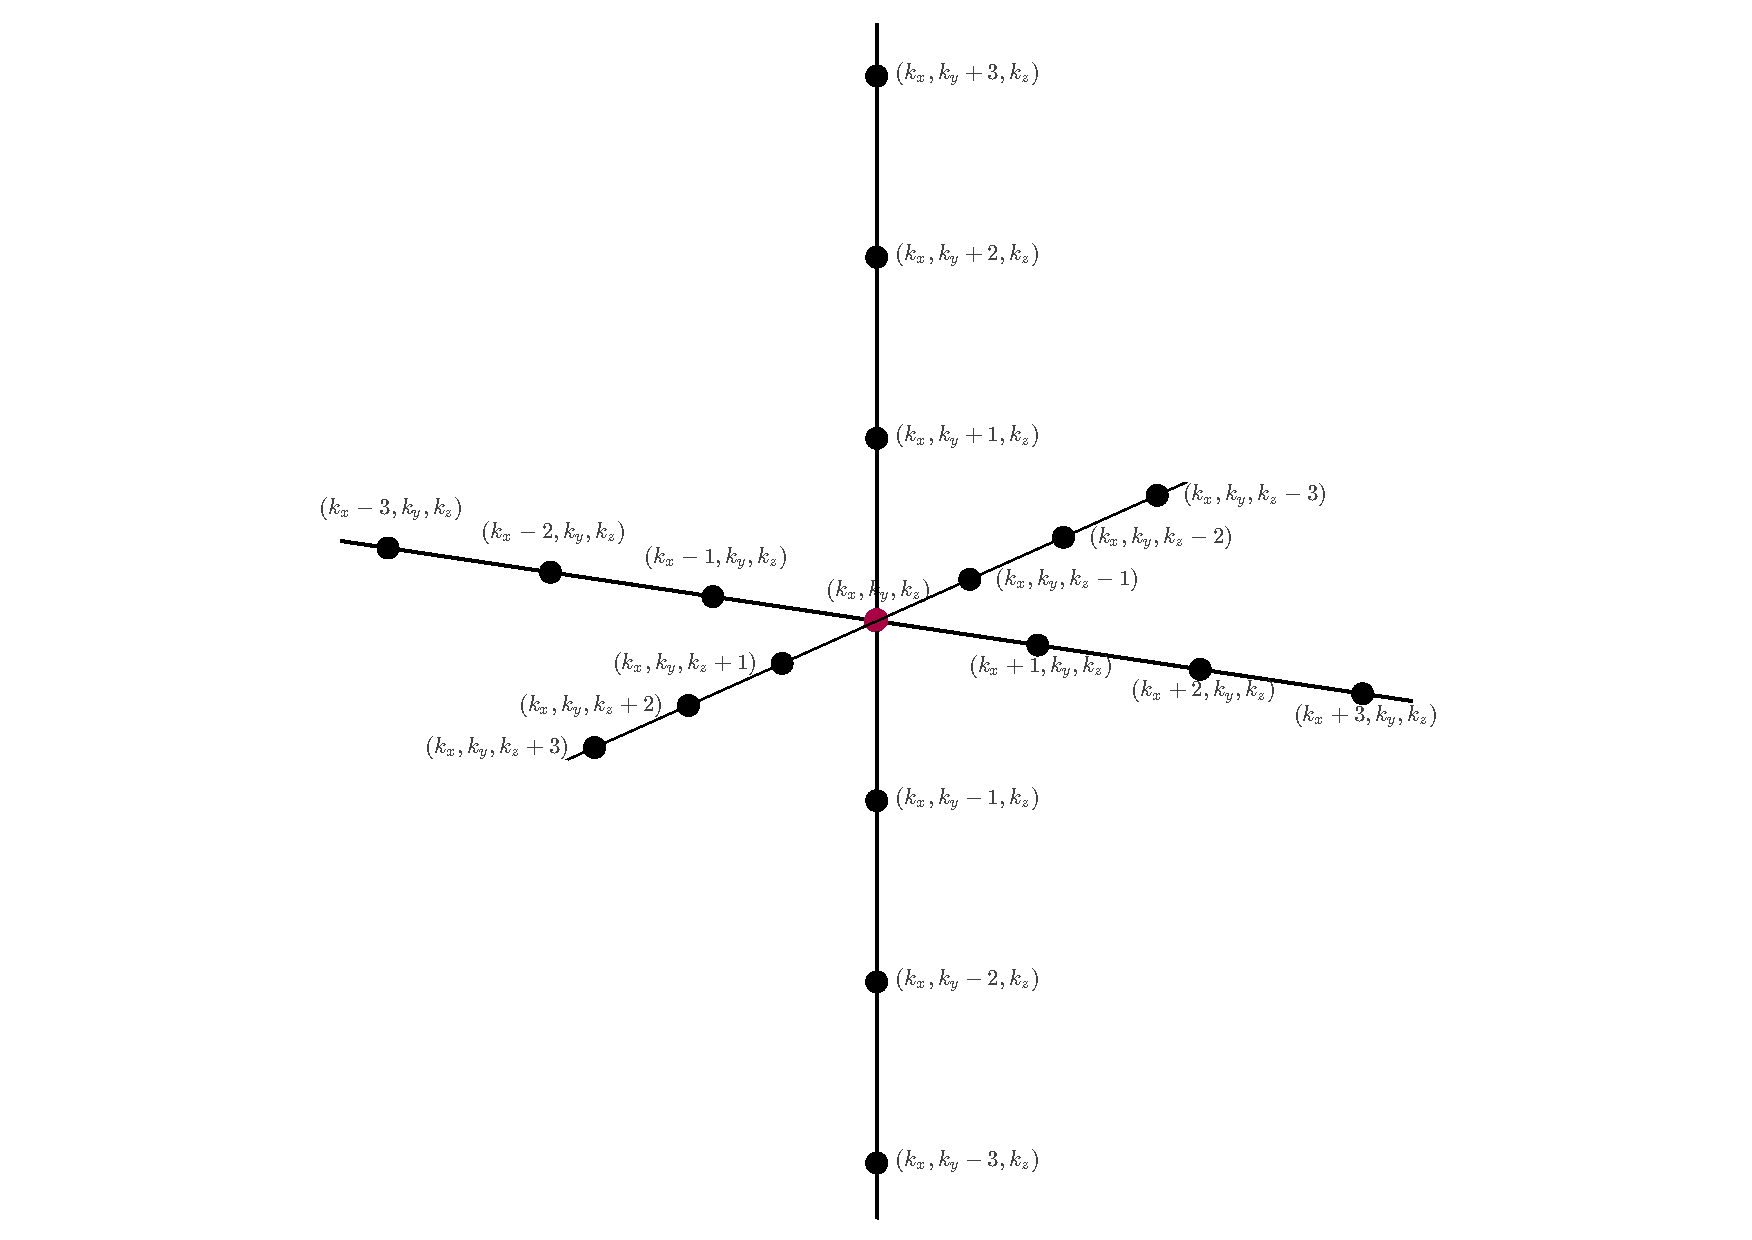
\includegraphics[width=0.9\textwidth]{\localPath/figures/stencil.pdf}
  \caption{Présentation des \emph{stencils} utilisés par la méthode WENO5 pour calculer le flux numérique.}
  \label{fig:intro:stencil}
\end{figure}

La méthode WENO5 consiste en 3 interpolations, sur 3 \emph{stencils} différents, comme l'illustre la figure~\ref{fig:intro:stencil}, pondérées par des poids non-linéaires issus des approximations des dérivées successives de $f$. L'écriture des poids s'effectue comme suit dans le cas $f^-=0$ :
$$
  \begin{aligned}
    \beta_0 &= \frac{13}{12}( \underbrace{f^+_{j-2} - 2f^+_{j-1} + f^+_{j}}_{\Delta x^2(f''_{j} + \mathcal{O}(\Delta x))})^2   + \frac{1}{4}( \underbrace{  f^+_{j-2} - 4f^+_{j-1} + 3f^+_{j}  }_{ 2\Delta x ( f'_{j} + \mathcal{O}(\Delta x^2))})^2 \\
    \beta_1 &= \frac{13}{12}( \underbrace{f^+_{j-1} - 2f^+_{j}   + f^+_{j+1}}_{\Delta x^2(f''_{j} + \mathcal{O}(\Delta x^2))} )^2 + \frac{1}{4}( \underbrace{  f^+_{j-1} -               f^+_{j+1}}_{ 2\Delta x   f'_{j} + \mathcal{O}(\Delta x^2))})^2 \\
    \beta_2 &= \frac{13}{12}( \underbrace{f^+_{j}   - 2f^+_{j+1} + f^+_{j+2}}_{\Delta x^2(f''_{j} + \mathcal{O}(\Delta x))} )^2   + \frac{1}{4}( \underbrace{ 3f^+_{j}   - 4f^+_{j+1} +  f^+_{j+2}}_{-2\Delta x ( f'_{j} + \mathcal{O}(\Delta x^2))})^2 \\
  \end{aligned}
$$
où les coefficients $\beta_0$ sont appelés indicateurs de continuité (\emph{indicators of smoothness}). Ce qui nous permet de calculer les poids définis par :
$$
  \alpha_i = \frac{\gamma_i}{(\varepsilon + \beta_i)^2},\quad i=0,1,2
$$
où $\varepsilon$ est un paramètre numérique pour assurer la non nullité du dénominateur, il sera pris à $10^{-6}$ ; et avec $\gamma_0=\frac{1}{10}$, $\gamma_1=\frac{6}{10}$ et $\gamma_2=\frac{3}{10}$. La normalisation des poids s'effectue comme suit :
$$
  w_i = \frac{\alpha_i}{\sum_m \alpha_m},\quad i=0,1,2
$$
Nous pouvons ensuite calculer les flux numériques pour WENO5 \cite{Shu:2003}, donnés par :
$$
  \begin{aligned}
    \hat{f}_{j+\frac{1}{2}}^+   =\ & w_0\left(  \frac{2}{6}f^+_{j-2} - \frac{7}{6}f^+_{j-1} + \frac{11}{6}f^+_{j}   \right)
                                +    w_1\left( -\frac{1}{6}f^+_{j-1} + \frac{5}{6}f^+_{j}   +  \frac{2}{6}f^+_{j+1} \right) \\
                                +  & w_2\left(  \frac{2}{6}f^+_{j}   + \frac{5}{6}f^+_{j+1} -  \frac{1}{6}f^+_{j+2} \right).
  \end{aligned}
$$
La méthode WENO5 prend la forme finale :
$$
  \partial_xf(x_j) \approx \frac{1}{\Delta x}\left[ \left(\hat{f}_{j+\frac{1}{2}}^+ - \hat{f}_{j-\frac{1}{2}}^+ \right) + \left(\hat{f}_{j+\frac{1}{2}}^- - \hat{f}_{j-\frac{1}{2}}^- \right) \right].
$$

Il existe des variantes de la méthode WENO5, permettant de réduire la perte d'ordre à l'approche d'un choc, à savoir WENO-M (\cite{Henrick:2005}) ou WENO-Z (\cite{Borges:2008}). Ces variations se font sur le calcul des poids non-linéaires. Ainsi la méthode WENO-M utilise une fonction de \emph{mappage} pour équilibrer les poids et est définie par :
$$
  \begin{aligned}
    \alpha_i    &= \frac{\gamma_i}{(\epsilon + \beta_i)^2} \\
    \tilde{w}_i &= \frac{\alpha_i}{\sum_k \alpha_k} \\
    g_i         &= w_i\left( \frac{\gamma_i + \gamma_i^2 - 3w_i\gamma_i + w_i^2}{\gamma_i^2 + w_i(1-2\gamma_i)} \right) \\
    w_i         &= \frac{g_i}{\sum_k g_k}
  \end{aligned}
$$
avec le paramètre $\epsilon = 10^{-4}$. La méthode WENO-Z est quant à elle définie par :
$$
  \begin{aligned}
    \alpha_i &= \gamma_i\left( 1+ \frac{\tau_5}{\epsilon + \beta_i} \right) \\
    w_i      &= \frac{\alpha_i}{\sum_k \alpha_k}
  \end{aligned}
$$
avec les paramètres $\epsilon = 10^{-40}$ et $\tau_5 = \beta_0 - \beta_2$. Cette dernière méthode est celle qui réduit le plus la perte d'ordre à l'approche d'une discontinuité. L'étude approfondie de ces méthodes n'est pas envisagée dans ce travail car les solutions de la physique des plasmas ne présentent pas de discontinuités. Il est à noter que ces méthodes conservent la même linéarisation que le schéma WENO5 classique de Jiang et Shu~\cite{Jiang:1996}, ce qui permet d'y appliquer les résultats de stabilités obtenus dans le chapitre~\ref{chap1}.

Il est possible de monter en ordre en suivant les résultats dans~\cite{Wu:2021}, l'ordre 5 sera considéré comme suffisant dans la suite de ce travail.

L'étude de la stabilité de la méthode WENO5 couplée avec différentes méthodes de type Runge-Kutta pour la résolution en temps a été initiée dans~\cite{Wang:2007} où il a été démontré l'instabilité de la méthode couplée avec la méthode d'Euler explicite, il est nécessaire d'avoir au moins un étage supplémentaire permettant d'assurer la stabilité, ou d'utiliser une méthode d'ordre 3. Des estimations de stabilité et de conditions de stabilité ont par la suite été proposées dans \cite{Motamed:2010,Lunet:2017}. Une étude automatique de la stabilité est présentée dans~\cite{Crouseilles:2019b} qui constitue le chapitre~\ref{chap1} de ce document.

% --------------------------------------------------------------------
\subsection{Méthode semi-lagrangienne}
% --------------------------------------------------------------------

Une méthode très populaire pour la résolution numérique de l'équation de Vlasov est la méthode semi-lagrangienne. Celle-ci s'adapte très bien à notre problème car les termes de transports sont linéaires. Elle a l'avantage de ne pas introduire de contrainte de stabilité. La méthode semi-lagrangienne repose sur la remonté des caractéristique, prenons pour exemple l'équation :
$$
  \partial_t u + a\partial_xu = 0,\quad u(t=0,x)=u_0(x),
$$
ce qui correspond à l'équation~\ref{eq:0:dtudxfu} avec le flux $f$ linéaire par rapport à l'inconnue $u$. On définit les caractérisitique le long desquelles $u$ est constante :
$$
  \begin{cases}
    \dot{x}(s) = a \\
    x(t) = x
  \end{cases}
$$
dont la solution s'écrit $x(s) = a(s-t)+x$. Avec $u(s,x(s))=u(t,x(t))$ on a $u(s,a(s-t)+x) = u(t,x)$ et en prenant $s=t^n=n\Delta t$, et $t=t^{n+1}$, on a :
$$
  u(t^{n+1},x) = u(t^n,x-a\Delta t),\quad \forall x\in[0,L]
$$
Pour connaître $u(t^{n+1},x_j)$ de $u(t^n,\cdot)$, on pose $x=x_j$ : $u(t^{n+1},x_j) = u(t^n,x_j-a\Delta t)$, comme l'illustre la figure~\ref{fig:intro:semilag}. Dans le cadre d'un schéma numérique, $x_j-a\Delta t$ n'étant pas un point de la grille, il faut évaluer en $x_j-a\Delta t$ un polynôme par morceaux, construit à partir des données $u(t^n,x_k)$, $k\in\mathbb{N}$. Plusieurs méthodes d'interpolation sont alors envisageable, la méthode par splines permet une reconstruction gloable de la solution~\cite{Cheng:1976,Sonnendrucker:2015} ; une approche plus locale à partir des données d'un \emph{stencil}, c'est-à-dire des données $u(x_{j^\star-d},t^n)$ jusqu'à $u(x_{j^\star+d},t^n)$, à l'aide d'un polynôme d'interpolation, comme un polynôme de Lagrange de degré $2d+1$, est aussi envisageable~\cite{Charles:2013}. Nous utiliserons cette approche locale avec $d=2$ par la suite.

\begin{figure}[h]
  \centering
  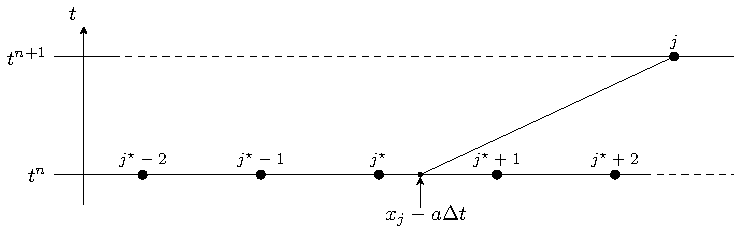
\includegraphics[width=0.9\textwidth]{\localPath/figures/semilag.pdf}
  \caption{Méthode des caractéristiques pour une méthode semi-lagrangienne avec une vitesse de transport $a>0$, et $d=2$.}
  \label{fig:intro:semilag}
\end{figure}


% --------------------------------------------------------------------
\subsection{Méthode pseudo-spectrale}
% --------------------------------------------------------------------

Une autre méthode souvent utilisée pour la résolution d'équations aux dérivées partielles est la méthode pseudo-spectrale qui consiste à approcher les opérateurs différentiels dans l'espace de Fourier à l'aide de transformées de Fourier. Cette méthode permet de transformer une équation aux dérivées partielles en un système d'équations différentielles ordinaires en transformant par exemple une dérivée dans l'espace réel en un produit dans l'espace de Fourier. Nous considèrerons ici la transformée de Fourier discrète, cela consiste à réécrire notre fonction $u$, $L$-périodique et de classe $C^1$, sous la forme :
$$
  u(x) = \sum_{\kappa=-\infty}^{+\infty} \hat{u}_\kappa e^{i\frac{2\pi \kappa}{L}x},
$$
où les coefficients de Fourier $\hat{u}_\kappa$ sont définis par :
$$
  \hat{u}_\kappa = \frac{1}{L}\int_0^L u(x)e^{-i\frac{2\pi \kappa}{L}x}\dd{x}.
$$

En n'ayant la connaissance de la fonction $u$ qu'en des points $x_j = j\frac{L}{N}$, $j=0,\dots,N-1$ de la grille, il est possible d'approcher les coefficient de Fourier par une somme discrète :
$$
  \hat{u}_\kappa \approx \frac{1}{N-1}\sum_{j=0}^N u(x_j) e^{=i\frac{2\pi j}{N}\kappa}.
$$

Transformer une dérivée en un produit nous sera utile au long de ce travail dans deux contextes, un premier linéaire :
$$
  \partial_t u + a\partial_x u = 0,\qquad u(t=0,x)=u_0(x)
$$
devenant après une transformée de Fourier : $\partial_t \hat{u}_\kappa + ai\kappa \hat{u}_\kappa = 0$ et pouvant se résoudre exactement en temps : $\hat{u}_\kappa(t) = \exp(-ia\kappa t)\hat{u}_\kappa(0)$. Cela correspond à la partie linéaire d'une méthode de Lawson~\ref{ssec:0:lawson}. L'autre cas d'utilisation sera pour un terme non-linéaire de la forme :
$$
  \partial_t u + \partial_xf(u) = 0,\qquad u(t=0,x)=u_0(x)
$$
devenant alors après une transformée de Fourier : $\partial_t\hat{u}_\kappa + i\kappa\widehat{\left(f(u)\right)}_\kappa = 0$. Ce terme n'ayant pas de solution explicite il sera résolu numériquement pas une méthode Runge-Kutta, correspondant au terme non-linéaire d'une méthode de Lawson.

Nous utiliserons l'algorithme de transformée de Fourier rapide (\emph{fast Fourier transform} ou FFT) pour effectuer numériquement cette opération, dont une implémentation est proposée dans~\cite{Saramito:2013}. Cet algorithme possède une complexité en temps de $\order{N\log N}$, où $N$ est le nombre de points de discrétisation en espace.

%% section 5
% !TEX root = ../../main.tex

\section{Relations de dispersion}
\label{s:dispersion}

Cette section est dédiée à l'étude des relations de dispersion relatives aux modèles cinétique~\eqref{eq:vlasov}-\eqref{eq:poisson} et hybride linéarisé~\eqref{eq:vahl}. Il s'agit de linéariser le modèle étudié puis d'exprimer le mode fondamental du champ électrique linéarisé. Cela permet d'obtenir une très bonne approximation de la phase linéaire de l'énergie électrique. Cette approche, complètement indépendante des schémas numériques utilisés pour résoudre le modèle de départ, sera utilisée comme outil de validation des codes présentés dans la section~\ref{s:scheme}.

Nous allons présenter les relations de dispersion de nos deux modèles, puis nous expliquerons comment reconstruire l'approximation linéaire de l'énergie électrique. Enfin, nous détaillerons les calculs des relations de dispersion pour le cas test qui nous intéressera dans les simulations numériques (sections~\ref{s:limit} et~\ref{s:compare}).

%----------
\subsection{Relations de dispersion dans le cas cinétique}
%----------

Nous nous intéressons d'abord aux relations de dispersion du modèle cinétique de Vlasov-Poisson~\eqref{eq:vlasov}-\eqref{eq:poisson}, en nous appuyant sur \cite{Sonnendrucker:2015}. Pour obtenir les relations de dispersion, il est nécessaire de linéariser le système autour d'un équilibre, pour cela rappelons les équations de Vlasov-Poisson~\eqref{eq:vlasov}-\eqref{eq:poisson} :
\begin{equation}
  \begin{cases}
    \partial_t f + v\partial_xf + E\partial_vf = 0 \\
    \partial_x E = \int_\mathbb{R} f\,\mathrm{d}v - 1 \\
    f(t=0, x, v)=f^0(x,v)
  \end{cases}
  \label{eq:vp}
\end{equation}
Dans un premier temps, nous nous intéressons à la linérarisation de ce modèle cinétique autour d'un état d'équilibre donné par $\left(f(t,x,v)\right)_{eq} = f^{(0)}(v)$ et $\left(E(t,x)\right)_{eq} = 0$, on considère le développement suivant :
\begin{equation}
  \begin{cases}
    f(t,x,v) = f^{(0)}(v) + \varepsilon f^{(1)}(t,x,v) + \mathcal{O}(\varepsilon^2) \\
    E(t,x) = 0 + \varepsilon E^{(1)}(t,x) + \mathcal{O}(\varepsilon^2)
  \end{cases}
  \label{eq:expansions}
\end{equation}
La densité de particules est définie par $\rho_0 = \rho_{0,c}+\rho_{0,h} = \int f^{(0)}\,\mathrm{d}v$. On injecte~\eqref{eq:expansions} dans~\eqref{eq:vp} pour obtenir :
$$
  \begin{cases}
    \varepsilon\partial_t f^{(1)} + v\varepsilon\partial_x f^{(1)} + \varepsilon E^{(1)}\left(\partial_v f^{(0)}+\varepsilon\partial_v f^{(1)}\right)=\mathcal{O}(\varepsilon^2) \\
    \varepsilon\partial_x E^{(1)} = \int f^{(0)} + \varepsilon\int f^{(1)} - n_0 + \mathcal{O}(\varepsilon^2)
  \end{cases}
$$
ce qui nous permet d'obtenir, en négligeant les termes d'ordre $\varepsilon^2$, le système de Vlasov-Poisson linéarisé :
\begin{equation}
  \begin{cases}
    \partial_t f^{(1)} + v\partial_x f^{(1)} + E^{(1)}\partial_v f^{(0)} = 0 \\
    \partial_x E^{(1)} = \int f^{(1)}\,\mathrm{d}v
  \end{cases}
  \label{eq:systVPlin}
\end{equation}

Pour un état d'équilibre connu $f^{(0)}(v)$, habituellement une distribution gaussienne, les inconnues de~\eqref{eq:systVPlin} sont $f^{(1)}(t,x,v)$ et $E^{(1)}(t,x)$.

Nous souhaitons dériver l'expression générale de la relation de dispersion associée au modèle cinétique linéarisé~\eqref{eq:systVPlin}. Afin de simplifier la lecture, nous supprimons l'index $(1)$ sur nos inconnues $f^{(1)}$ et $E^{(1)}$. Nous supposons que le fonctions $f^{(1)}$ et $E^{(1)}$ sont $L$-périodiques en $x$ dans le domaine $\Omega=[0,L]$, nous allons, successivement, appliquer une transformée de Fourier en $x$ et et une transformée de Laplace en $t$ sur le système~\eqref{eq:systVPlin}.

Tout d'abord, nous effectuons une transformée de Fourier en $x$, définie pour une fonction $f(x)$ comme :
$$
  \hat{f}(k) = \frac{1}{L}\int_0^L f(x)e^{-ikx}\,\mathrm{d}x\,,\quad k=\frac{2\pi}{L}n, n\in\mathbb{Z}
$$
Nous obtenons :
\begin{equation}
  \begin{cases}
    \partial_t \hat{f} + ikv\hat{f} + \hat{E}\partial_v f^{(0)} = 0 \\
    ik\hat{E} = \int \hat{f}(t,k,v) dv
  \end{cases}
  \label{eq:fourier}
\end{equation}
Maintenant, nous utilisons la transformée de Laplace définie pour une fonction $f(t)$ par :
$$
  \tilde{f}(\omega) = \int_0^{+\infty} f(t)e^{i\omega t}\,\mathrm{d}t
$$
et, si elle est définie, la transformée de Laplace inverse est donnée par :
$$
  f(t) = \frac{1}{2i\pi}\int_{u-i\infty}^{u+i\infty} \tilde{f}(\omega)e^{-i\omega t}\,\mathrm{d}\omega
$$
Appliquons la transformée de Laplace à la première équation du système~\eqref{eq:fourier} :
$$
  \int_0^{+\infty}\partial_t\hat{f}(t)e^{i\omega t}\,\mathrm{d}t
  + \int_0^{+\infty}ikv\hat{f}(t)e^{i\omega t}\,\mathrm{d}t
  + \int_0^{+\infty}\hat{E}(t)\partial_v f^{(0)}e^{i\omega t}\,\mathrm{d}t
  = 0
$$
et en utilisant une intégration par partie dans la première intégrale nous obtenons :
$$
  \begin{aligned}
    -\hat{f}(t=0,k,v) - i\omega\int_0^{+\infty} \hat{f}(t)e^{i\omega t}\,\mathrm{d}t + ikv\int_0^{+\infty} \hat{f}(t)e^{i\omega t} \mathrm{d}t \\
    +\partial_vf^0\int_0^{+\infty}\hat{E}(t)e^{i\omega t}\,\mathrm{d}t=0
  \end{aligned}
$$
et donc :
\begin{equation}
  (ikv-i\omega)\tilde{\hat{f}}(\omega,k,v) + \partial_vf^0\tilde{\hat{E}}(\omega,k) = \hat{f}_0(k,v),
  \label{eq:fourierlaplace_f}
\end{equation}
où $\hat{f}_0(k,v) = \hat{f}(t=0,k,v)$ correspond à la condition initiale. En appliquant maintenant la transformée de Laplace à la seconde équation de~\eqref{eq:fourier} nous obtenons :
$$
  \int_0^{+\infty}ik\hat{E}(t,k)e^{i\omega t}\,\mathrm{d}t = \int_0^{+\infty}\int_{-\infty}^{+\infty}\hat{f}(t,k,v)\,\mathrm{d}v\,e^{i\omega t}\,\mathrm{d}t
$$
ce qui nous donne :
\begin{equation}
  \tilde{\hat{E}}(\omega,k)=-\frac{i}{k}\int_{-\infty}^{+\infty}\tilde{\hat{f}}(\omega,k,v)dv
  \label{eq:fourierlaplace_E}
\end{equation}
Maintenant, nous souhaitons injecter l'équation~\eqref{eq:fourierlaplace_f} dans~\eqref{eq:fourierlaplace_E}. Nous devons prêter attention aux pôles $\omega = kv$. En fait, si $\Im(\omega)>0$ et pour une fonction analytique $g(v)$, alors l'intégrale $\int_{-\infty}^{+\infty}\frac{g(v)}{ikv-i\omega}\,\mathrm{d}v$ est analytique. Lorsque $\Im(\omega) \leq 0$, nous devons construire un prolongement analytique et remplacer l'intégrale par $\int_\gamma \frac{g(v)}{ikv-i\omega}\,\mathrm{d}v$ avec $\gamma$ un coutour ouvert parallèle à l'axe réel à l'infini et qui passe par le pôle $\omega = kv$ (voir \cite{Sonnendrucker:2015}). Par la suite, nous utiliserons la notation $\gamma$ soit pour l'axe réel $]-\infty,+\infty[$ quand $\Im(\omega)>0$, ou pour un chemin ouvert bien choisi lorsque $\Im(\omega)\leq 0$. 

Avec cette notation, le résultat de l'injection de~\eqref{eq:fourierlaplace_f} dans~\eqref{eq:fourierlaplace_E} nous donne :
$$
  \begin{aligned}
    \tilde{\hat{E}}
    & = -\frac{i}{k}\int_\gamma \frac{1}{ikv-i\omega}\left( \hat{f}_0(k,v) - \partial_vf^{(0)}\tilde{\hat{E}}(\omega,k) \right)\,\mathrm{d}v \\
    & = -\frac{1}{k}\int_\gamma \frac{\hat{f}_0(k,v)}{kv-\omega}\,\mathrm{d}v + \frac{1}{k}\int_\gamma \frac{\partial_v f^{(0)}\tilde{\hat{E}}(\omega,k)}{kv-\omega}\,\mathrm{d}v \\
    & = - \frac{1}{k^2}\int_\gamma \frac{\hat{f}_0(k,v)}{v-\frac{\omega}{k}}\,\mathrm{d}v + \frac{1}{k^2}\tilde{\hat{E}}(\omega,k)\int_\gamma \frac{\partial_v f^{(0)}}{v-\frac{\omega}{k}}\,\mathrm{d}v
  \end{aligned}
$$
donc :
$$
  \left( 1 - \frac{1}{k^2}\int_\gamma \frac{\partial_v f^{(0)}}{v-\frac{\omega}{k}}\,\mathrm{d}v \right) \tilde{\hat{E}}(\omega,k) = -\frac{1}{k^2}\int_\gamma \frac{\hat{f}_0(k,v)}{v-\frac{\omega}{k}}\,\mathrm{d}v
$$
En introduisant :
\begin{equation}
  D(k,\omega) = 1 - \frac{1}{k^2}\int_\gamma \frac{\partial_v f^{(0)}}{v-\frac{\omega}{k}}\,\mathrm{d}v
  \label{eq:D}
\end{equation}
et
\begin{equation}
  N(k,\omega) = -\frac{1}{k^2}\int_\gamma\frac{\hat{f}_0(k,v)}{v-\frac{\omega}{k}}dv
  \label{eq:N}
\end{equation}
nous pouvons définir $\tilde{\hat{E}}(\omega,k)$ comme :
$$
  \tilde{\hat{E}}(\omega,k) = \frac{N(k,\omega)}{D(k,\omega)}
$$
L'équation~\eqref{eq:D} est appelée relation de dispersion du modèle cinétique.

%----------
\subsection{Relations de dispersion dans le cas hybride}
%----------

Intéressons-nous dans cette section à dériver l'expression générale de la relation de dispersion associée au modèle hybride linéarisé~\eqref{eq:vahl}. Pour cela, nous allons repartir du modèle hybride non-linéaire~\eqref{eq:hyb_nonlin} et linéariser à la fois les équations fluides et l'équation cinétique. On injecte le développement~\eqref{eq:lin_variables} dans~\eqref{eq:hyb_nonlin}. Les mêmes calculs que dans la section~\ref{s:models} et l'approximation en $\varepsilon^2$ y compris dans l'équation cinétique sur $f_h$ conduisent au modèle
$$
  \begin{cases}
    \partial_tu_c^{(1)}=E^{(1)}\\
    \partial_tE^{(1)}=-\rho_c^{(0)}u_c^{(1)}-\int v f_h^{(1)}\,\mathrm{d}v\\
    \partial_t f_h^{(1)}+ v\partial_xf_h^{(1)}+ E^{(1)}\partial_vf_h^{(0)}=0
  \end{cases}
$$ 
d'inconnues $E^{(1)}$, $u_c^{(1)}$ et $f_h^{(1)}$ que nous noterons dans la suite, respectivement, $E$, $u_c$ et $f_h$, solutions du système hybride linéarisé dans toutes les inconnues
\begin{equation}
  \begin{cases}
    \partial_t u_c = E \\
    \partial_t E = -\rho_c^{(0)}u_c - \int vf_h\,\mathrm{d}v \\
    \partial_t f_h + v\partial_x f_h + E\partial_v f_h^{(0)} = 0
  \end{cases}
\label{eq:systHlin}
\end{equation}
Nous insistons sur le fait que le modèle~\eqref{eq:systHlin} correspond à une linéarisation de la partie cinétique (ou chaude) du modèle hybride~\eqref{eq:vahl} que nous avons étudié précédemment. Par la suite, nous supposerons que la densité de particules froides $\rho_c^{(0)}$ est une constante (en temps $t$ et espace $x$) et que la fonction $f_h^{(0)}$ est une fonction paire en $v$ et ne dépend que de cette variable. Nous supposons que les fonctions $f_h$, $E$ et $u_c$ sont $L$-périodiques en $x$ sur le domaine spatial $\Omega = [0,L]$ et nous appliquons la transformée de Fourier en $x$ puis une transformée de Laplace en $t$.

Tout d'abord, nous appliquons la transformée de Fourier en $x$ :
\begin{equation}
  \begin{cases}
    \partial_t \hat{u}_c = \hat{E} \\
    \partial_t\hat{E}=-\rho_c^{(0)}\hat{u}_c-\int \hat{f}_h dv \\
    \partial_t \hat{f}_h+ikv\hat{f}_h+ \hat{E}\partial_v f_h^{(0)} = 0
  \end{cases}
  \label{eq:fourierH}
\end{equation}
Alors, nous multiplions par $e^{i\omega t}$ et nous intégrons en temps. L'équation sur $\hat{u}_c$ nous donne :
\begin{eqnarray}
  \int_0^{+\infty} \partial_t \hat{u}_c e^{i\omega t} \,\mathrm{d}t &=& \int_0^{+\infty} \hat{E}e^{i\omega t}\,\mathrm{d}t\nonumber\\
  -\int_0^{+\infty}i\omega  \hat{u}_c e^{i\omega t} \,\mathrm{d}t-\hat{u}_c(t=0,k) &=& \int_0^{+\infty} \hat{E}e^{i\omega t}\,\mathrm{d}t\nonumber\\
  -i\omega  \tilde{\hat{u}}_c(\omega,k)-\hat{u}_c(t=0,k) &=& \tilde{\hat{E}}(\omega,k)\nonumber\\
  \tilde{\hat{u}}_c(\omega,k)+\frac{1}{i\omega}\tilde{\hat{E}}(\omega,k) &=& -\frac{1}{i\omega}\hat{u}_c(t=0,k)
  \label{eq:LF_u}
\end{eqnarray}
Les mêmes opérations sur l'équation sur $\hat{E}$ nous donnent :
\begin{eqnarray}
  -i\omega  \tilde{\hat{E}}(\omega,k)-\hat{E}(t=0,k)&=&-\rho_c^{(0)}\tilde{\hat{u}}_c(\omega,k)-\int_{-\infty}^{+\infty} v\tilde{\hat{f}}_h(\omega,k)dv
  \label{eq:LF_E}
\end{eqnarray}
Tandis que l'équation sur $\hat{f}_h$ nous donne :
\begin{eqnarray}
  -i\omega  \tilde{\hat{f}}_h(\omega,k,v)-\hat{f}_h(t=0,k,v)+ikv\tilde{\hat{f}}_h(\omega,k,v)+\tilde{\hat{E}}(\omega,k)\partial_vf_h^{(0)}(v)=0\nonumber\\
  \tilde{\hat{f}}_h(\omega,k,v)\left(ikv-i\omega\right)=\hat{f}_h(t=0,k,v)-\tilde{\hat{E}}(\omega,k)\partial_vf_h^{(0)}(v)\nonumber\\
  \tilde{\hat{f}}_h(\omega,k,v)=-\frac{i}{k}\frac{\hat{f}_h(t=0,k,v)}{v-\frac{\omega}{k}}+\frac{i}{k}\frac{\tilde{\hat{E}}(\omega,k)\partial_vf_h^{(0)}(v)}{v-\frac{\omega}{k}}.
  \label{eq:LF_f}
\end{eqnarray}
Nous injectons l'expression~\eqref{eq:LF_f} dans~\eqref{eq:LF_E} :
$$
  \begin{aligned}
    -i\omega  \tilde{\hat{E}}(\omega,k)-\hat{E}(t=0,k)=-\rho_c^{(0)}\tilde{\hat{u}}(\omega,k)+\frac{i}{k}\int_\gamma v\frac{\hat{f}_h(t=0,k,v)}{v-\frac{\omega}{k}}dv \\
    -\frac{i}{k}\int_\gamma v\frac{\tilde{\hat{E}}(\omega,k)\partial_vf_h^{(0)}(v)}{v-\frac{\omega}{k}}dv
  \end{aligned}
$$
soit :
\begin{equation}
  \begin{aligned}
    \tilde{\hat{E}}(\omega,k)\left(1-\frac{1}{\omega k}\int_\gamma v\frac{\partial_vf_h^{(0)}(v)}{v-\frac{\omega}{k}}dv\right)-\frac{\rho_c^{(0)}}{i\omega}\tilde{\hat{u}}_c(\omega,k)=-\frac{1}{i\omega}\hat{E}(t=0,k)\nonumber\\
    -\frac{1}{\omega k}\int_\gamma v\frac{\hat{f}_h(t=0,k,v)}{v-\frac{\omega}{k}}dv
  \end{aligned}
  \label{eq:LF_Ef}
\end{equation}
Nous injectons maintenant l'expression~\eqref{eq:LF_u} dans~\eqref{eq:LF_Ef} pour obtenir le problème suivant :
$$
  \begin{aligned}
    \tilde{\hat{E}}(\omega,k)\left(1-\frac{1}{\omega k}\int_\gamma v\frac{\partial_vf_h^{(0)}(v)}{v-\frac{\omega}{k}}dv\right)+\frac{\rho_c^{(0)}}{i\omega}\left(\frac{1}{i\omega}\tilde{\hat{E}}(\omega,k)+\frac{1}{i\omega}\hat{u}_c(t=0,k)\right)\\
    =-\frac{1}{i\omega}\hat{E}(t=0,k)
    -\frac{1}{\omega k}\int_\gamma v\frac{\hat{f}_h(t=0,k,v)}{v-\frac{\omega}{k}}dv
  \end{aligned}
$$
soit :
$$
  \begin{aligned}
    \tilde{\hat{E}}(\omega,k)\left(1-\frac{1}{k^2}\left(\rho_c\frac{k^2}{\omega^2}+\int_\gamma \frac{\partial_vf_h^{(0)}(v)}{v-\frac{\omega}{k}}dv\right)\right)~~~~~~~~~~~~~~~~~~~~~~~~~~~~~~~~~~~~~~~~\\
    =\frac{\rho_c^{(0)}}{\omega^2}\hat{u}_c(t=0,k)-\frac{1}{i\omega}\hat{E}(t=0,k)
    -\frac{1}{\omega k}\int_\gamma v\frac{\hat{f}_h(t=0,k,v)}{v-\frac{\omega}{k}}dv
  \end{aligned}
$$
Nous introduisons :
\begin{equation}
  D(k,\omega) = 1-\frac{1}{k^2}\left( \rho_c^{(0)}\frac{k^2}{\omega^2}+\int_\gamma \frac{\partial_vf_h^{(0)}(v)}{v-\frac{\omega}{k}}dv\right )
  \label{eq:relD_H}
\end{equation}
et
\begin{equation}
  N(k,\omega) = \frac{\rho_c^{(0)}}{\omega^2}\hat{u}_c(t=0,k)-\frac{1}{i\omega}\hat{E}(t=0,k) 
    -\frac{1}{\omega k}\int_\gamma v\frac{\hat{f}_h(t=0,k,v)}{v-\frac{\omega}{k}}dv,
  \label{eq:relN_H}
\end{equation}
nous pouvons alors définir $\tilde{\hat{E}}(\omega,k)$ comme :
$$
  \tilde{\hat{E}}(\omega,k)=\frac{N(k,\omega)}{D(k,\omega)}
$$

\begin{remark}
  Comme nous le verrons dans la sous-section suivante, pour retrouver la pente de la partie linéaire de l'énergie électrique, il est suffisant de trouver les racines de $D(k,\omega)$, ou les pôles de $\tilde{\hat{E}}(\omega,k)$. Si seule la pente de la partie linéaire nous intéresse, un autre moyen de la retrouver est de réécrire les équations~\eqref{eq:LF_u}-\eqref{eq:LF_Ef} comme le système suivant :
  \begin{equation}
    \begin{pmatrix}
      1                       & \frac{1}{i\omega} \\
      -\frac{\rho_c}{i\omega} & 1-\frac{1}{\omega k}\int_\gamma v\frac{\partial_v f_h^{(0)}(v)}{v-\frac{\omega}{k}}\,\mathrm{d}v
    \end{pmatrix}
    \begin{pmatrix}
      \tilde{\hat{u}}_c(\omega,k) \\
      \tilde{\hat{E}}(\omega,k)
    \end{pmatrix}
    =
    \begin{pmatrix}
      -\frac{1}{i\omega}\hat{u}_c(0,k) \\
      -\frac{1}{i\omega}\hat{E}(0,k) - \frac{1}{\omega k}\int_\gamma v\frac{\hat{f}_h(0,k,v)}{v-\frac{\omega}{k}}\,\mathrm{d}v
    \end{pmatrix}
    \label{eq:systHyb}
  \end{equation}
  Le problème revient alors à trouver les racines du déterminant de ce système, qui s'écrit
%  Nous sommes alors incités à calculer le déterminant de ce système pour se faire une idée des solutions de ce système :
  $$
    \begin{aligned}
      Det(k,\omega) & = 1 - \frac{1}{\omega k}\int_\gamma v\frac{\partial_v f_h^{(0)}(v)}{v-\frac{\omega}{k}}\,\mathrm{d}v - \frac{\rho_c^{(0)}}{\omega^2} \\
                    & = 1 - \frac{1}{k^2}\left( \rho_c^{(0)}\frac{k^2}{\omega^2} + \int_\gamma \frac{\partial_v f_h^{(0)}(v)}{v-\frac{\omega}{k}}\,\mathrm{d}v \right)
    \end{aligned}
  $$
  On retrouve bien~\eqref{eq:relD_H}. La connaissance de~\eqref{eq:relN_H} nous donnera, en plus de la pente, la phase de l'énergie électrique dans sa partie linéaire.
\end{remark}

%----------
\subsection{Expression du champ électrique linéarisé}
%----------

Dans cette sous-section, nous considérons un prolongement analytique continu de $N(k,\omega)$ et $D(k,\omega)$, et nous supposons que la transformée de Laplace et de Fourier de $\tilde{\hat{E}}$ sont bien définies pour obtenir une approximation du champ électrique linéarisé.

La transformée de Laplace inverse peut être calculée à l'aide du théorème des résidus :
$$
  \hat{E}(t,k)=\frac{1}{2i\pi}\int_{u-i\infty}^{u+i\infty}\tilde{\hat{E}}(\omega,k)e^{-i\omega t}d\omega=\sum_jRes_{\omega=\omega^{k,j}}\left(\tilde{\hat{E}}(\omega,k)e^{-i\omega t}\right)
$$
où $\omega^{k,j}$ sont les pôles de $\tilde{\hat{E}}(\omega,k)$. Nous rappelons que si $\omega^{k,j}$ est un pôle simple, alors :
$$
  \begin{aligned}
    Res_{w=w^{k,j}}\left( \tilde{\hat{E}}(\omega,k)e^{-i\omega^{k,j}t} \right)
      & = \lim_{\omega\to\omega^{k,j}}\left( \omega - \omega^{k,j} \right)\tilde{\hat{E}}(\omega,k)e^{-i\omega t} \\
      & = \lim_{\omega\to\omega^{k,j}}\left( \omega - \omega^{k,j} \right)\frac{N(k,\omega)}{D(k,\omega)}e^{-i\omega t}
  \end{aligned}
$$
Maintenant, un développement de Taylor de $D(k,\omega)$ nous donne :
$$
  D(k,\omega) = \underbrace{D(k,\omega^{k,j})}_{0} + \left( \omega - \omega^{k,j} \right)\frac{\partial D}{\partial \omega}(k,\omega^{k,j}) + \mathcal{O}\left( (\omega-\omega^{k,j})^2 \right)
$$
donc, le passage à la limite nous donne :
\begin{equation}
  Res_{\omega=\omega^{k,j}}\left(\tilde{\hat{E}}(\omega,k)e^{-i\omega^{k,j}t}\right)=\frac{N(k,\omega^{k,j})}{\frac{\partial D}{\partial \omega}(k,\omega^{k,j})}e^{-i\omega^{k,j} t}.
  \label{eq:residu}
\end{equation}

\begin{remark}
  En fait, pour un $k$ fixé, on obtient une très bonne approximation de $\hat{E}(t,k)$ (excepté pour des temps courts) en considérant seulement la fréquence principale. Soient les deux racines $\omega^{k,j_0\pm}=\pm\omega_r+i\omega_i$ de $D(k,\omega)$ (où $\omega_r\in\mathbb{R}^+$, $\omega_i\in\mathbb{R}$) qui ont la plus grande partie imaginaire $\omega_i$ : pour toute autre racine $\omega^{k,j}$, on a $\Im(\omega^{k,j})<\omega_i$. Les autres pôles peuvent être négligés. En effet, nous avons :
  $$
    \begin{aligned}
       \hat{E}(t,k)&=&\sum_jC_je^{-i\omega^{k,j} t}=C_{j_0^+}e^{-i\omega^{k,j_0^+}t}+C_{j_0^-}e^{-i\omega^{k,j_0^-}t}+\sum_{j\neq j_0^\pm}C_je^{-i\omega^{k,j} t}\\
 &=&e^{\omega_it}\left(C_{j_0^+}e^{-i\omega_rt}+C_{j_0^-}e^{i\omega_rt}+\sum_{j\neq j_0^\pm}C_je^{-i\Re(\omega^{k,j}) t}e^{(\Im(\omega^{k,j})-\omega_i)t}\right)
    \end{aligned}
  $$
  et par hypothèse, $\Im(\omega^{k,j})-\omega_i < 0$ $\forall j\neq j_0^\pm$, nous pouvons conclure que la somme tend vers zéro lorsque $t\to+\infty$.
\end{remark}

\begin{lemma}
  Si $f^{(0)}(v)$ (respectivement $f_h^{(0)}(v)$) est une fonction paire, alors pour $D$ défini par~\eqref{eq:D} (respectivement~\eqref{eq:relD_H}) nous avons $D(k,\omega_r+i\omega_i) = 0 \Leftrightarrow D(k,-\omega_r+i\omega_i)=0$.
  \label{lemma:doubleracine}
\end{lemma}
\begin{proof}
  Voir en Annexe~\ref{a:dispersion}. \commentaire[Anais]{(à voir si on le laisse en annexe ou si on l'enlève complètement)} 
\end{proof}

En considérant seulement les deux racines principales $\pm\omega_r + i\omega_i$ de $D(k,\omega)$, supposés pôles simples de $\tilde{\hat{E}}(\omega,k)$, nous avons l'approximation :
$$
  \hat{E}(t,k)\approx Res_{\omega=\omega_r+i\omega_i}\left(\tilde{\hat{E}}(\omega,k)e^{-i\omega t}\right)+Res_{\omega=-\omega_r+i\omega_i}\left(\tilde{\hat{E}}(\omega,k)e^{-i\omega t}\right)
$$
où les résidus sont définis par~\eqref{eq:residu}. Notons $r^\pm$ le module de $\frac{N(k,\pm\omega_r+i\omega_i)}{\frac{\partial D}{\partial \omega}(k,\pm\omega_r+i\omega_i)}$ et $\phi^\pm$ son argument, nous avons alors :
\begin{equation}
  \hat{E}(t,k)\approx r^+e^{i\phi^+}e^{-i(\omega_r+i\omega_i)t}+r^-e^{i\phi^-}e^{-i(-\omega_r+i\omega_i)t}. 
  \label{eq:Etk_sanssym}
\end{equation}
Dans plusieurs cas test classiques, nous avons une symétrie entre les racines, qui dépend de la perturbation initiale de l'équilibre. Par la suite la perturbation initiale de l'équilibre sera toujours une fonction cosinus.

\begin{hyp}
  Le module et l'argument de $\frac{N(k,\pm\omega_r+i\omega_i)}{\frac{\partial D}{\partial \omega}(k,\pm\omega_r+i\omega_i)}$  vérifient $r^+ = r^-$ (noté $r$ par la suite) et $\phi^+ = -\phi^-$ (noté simplement $\phi$).
  \label{hyp:sym}
\end{hyp}
Sous l'hypothèse~\ref{hyp:sym}, nous obtenons :
\begin{eqnarray}
  \hat{E}(t,k)\approx&& re^{i\phi}e^{-i(\omega_r+i\omega_i)t}+re^{-i\phi}e^{-i(-\omega_r+i\omega_i)t} \nonumber\\
  &=&re^{\omega_i t}\left(e^{i(\omega_r t-\phi)}+e^{-i(\omega_r t-\phi)}\right)\nonumber\\
  &=&2re^{\omega_i t}\cos\left(\omega_r t-\phi\right).
  \label{eq:Etk}
\end{eqnarray}
Maintenant, si nous considérons la définition des coefficients de Fourier, nous avons :
$$
  \hat{E}(t,k) = \frac{1}{L}\int_0^L E(t,x)e^{-ikx}\,\mathrm{d}x = \frac{1}{L}\int_0^L E(t,x)\cos(-kx)\,\mathrm{d}x + i\frac{1}{L}\int_0^L E(t,x)\sin(-kx)\,\mathrm{d}x
$$
et :
$$
  \begin{aligned}
    \hat{E}(t,-k) 
      & = \frac{1}{L}\int_0^L E(t,x)e^{ikx}\,\mathrm{d}x = \frac{1}{L}\int_0^L\cos(kx)\,\mathrm{d}x + i\frac{1}{L}\int_0^L E(t,x)\sin(kx)\,\mathrm{d}x \\
      & = \frac{1}{L}\int_0^L E(t,x)e^{ikx}\,\mathrm{d}x = \frac{1}{L}\int_0^L\cos(-kx)\,\mathrm{d}x - i\frac{1}{L}\int_0^L E(t,x)\sin(-kx)\,\mathrm{d}x \\
      & = \overline{\hat{E}(t,k)}
  \end{aligned}
$$

\begin{hyp}
  $N(k,\omega) = 0$ si $k\notin\left\{\pm\frac{2\pi}{L}\right\}$.
  \label{hyp:knuls}
\end{hyp}
Sous l'hypothèse~\ref{hyp:knuls}, avec l'approximation des coefficients de Fourier (qui sont tous réels) données par~\eqref{eq:Etk} et avec $l=\frac{2\pi}{L}$, nous obtenons l'approximation du champ électrique suivante :
$$
  \begin{aligned}
    E(t,x) &\approx \varepsilon E^{(1)}(t,x) \approx \varepsilon\left( \hat{E}(t,l)e^{ikx} + \overline{\hat{E}(t,l)}e^{-ilx} \right) \\
           &\approx 2\varepsilon \hat{E}(t,l)\cos(lx) \\
           &\approx 4\varepsilon r e^{\omega_i t}\cos(\omega_t t -\phi)\cos\left(\frac{2\pi}{L}x\right)
  \end{aligned}
$$
Ce qui nous permet d'obtenir une approximation de l'énergie électrique, définie par :
\begin{equation}
  \begin{aligned}
    \mathcal{E}(t) & := \left( \int_0^L E^2(t,x)\,\mathrm{d}x \right)^{\frac{1}{2}} \\
                   & \approx 4\varepsilon r e^{\omega_i t}\left|\cos(\omega_rt - \phi)\right|\left( \int_0^L \cos^2\left(\frac{2\pi}{L}x\right)\,\mathrm{d}x \right)^{\frac{1}{2}} \\
                   & \approx 2\sqrt{2L}\varepsilon r e^{\omega_i t}\left|\cos(\omega_rt - \phi)\right|
  \end{aligned}
\label{eq:enelec}\end{equation}
puisque :
$$
  \begin{aligned}
    \int_0^L \cos^2\left(\frac{2\pi}{L}x\right)\,\mathrm{d}x
      & = \int_0^L\frac{1}{2}\,\mathrm{d}x + \int_0^L\frac{1}{2}\cos\left(\frac{4\pi}{L}x\right)\,\mathrm{d}x \\
      & = \frac{L}{2} + \left[ \frac{L}{8\pi}\sin\left(\frac{4\pi}{L}x\right)\right]_0^L = \frac{L}{2}
  \end{aligned}
$$

\begin{remark}
  Il est possible de mener une étude similaire pour une perturbation donnée par une fonction sinus. Nous obtenons alors des résultats similaires en remplaçant dans l'approximation de $\hat{E}(t,k)$, $E(t,x)$ et $\mathcal{E}(t)$ les fonctions cosinus par des fonctions sinus.
\end{remark}

Il est à noter que ces approximations ne prennent en compte que les racines dominantes de $D(\frac{2\pi}{L},\omega)$, les deux ayant la plus grande partie imaginaire. Cette approximation devient valable en temps $t$ suffisamment long.

La partie imaginaire $\omega_i$ nous donne le comportement global des coefficients de Fourier du champ électrique, et donc de l'énergie électrique comme une fonction du temps. Nous obtenons un amortissement de l'énergie électrique si $\omega_i < 0$, ou une instabilité si $\omega_i >0$. Lorsque nous traçons l'énergie électrique en fonction du temps en échelle logarithmique, nous pouvons observer les comportements suivants :
\begin{itemize}
  \item un amortissement avec un taux $\omega_i<0$, le taux indiquant la pente globale de l'amortissement,
  \item quelques oscillations stables, suivies du développement d'une instabilité avec un taux $\omega_i>0$, jusqu'à la saturation recherchée.
\end{itemize}

%----------
\subsection{Applications}\label{ssec:disp_appl}
%----------

Dans cette sous-section, nous nous intéressons au calcul de $D(k,\omega)$ pour le modèle cinétique~\eqref{eq:D} ou hybride~\eqref{eq:relD_H}, dans le cadre des cas tests qui nous intéressent. Pour le modèle cinétique la distribution initiale est donnée par :
$$
  f_0(x,v) = \mathcal{M}_{1-\alpha,0,T_c}(v)
    + \left(
      \mathcal{M}_{^\alpha/_2,v_0,1}(v) + \mathcal{M}_{^\alpha/_2,-v_0,1}(v)
    \right)(1+\epsilon\cos(kx))
$$
avec $\alpha$ la densité de particules chaudes, centrées en $\pm v_0\in\mathbb{R}$, et les particules froides sont caractérisées par une température $T_c$, et où l'on note :
$$
  \mathcal{M}_{\rho,u,T}(v) := \frac{1}{(2\pi T)^\frac{1}{2}}\exp\left(-\frac{|v-u|^2}{2T}\right)
$$
la distribution maxwellienne de densité $\rho$, centrée en la vitesse $u$ et de température $T$. Cette distribution initiale $f_0$ nous permet de construire une condition initiale compatible pour le modèle hybride, données par la limite $T_c\to 0$ :
\begin{equation}
  \begin{aligned}
    f_{h,0} (x,v) & = \left(
      \mathcal{M}_{^\alpha/_2,v_0,1}(v) + \mathcal{M}_{^\alpha/_2,-v_0,1}(v)
    \right)(1+\epsilon\cos(kx)) \\
    u_{c,0} & = 0
  \end{aligned}
\label{eq:f0hdexv}\end{equation}
le champ électrique à l'instant initial $E_0$ est donné par la résolution de l'équation de Poisson avec la condition initiale :
$$
  \partial_x E_0(x) = (1-\alpha) + \int_\mathbb{R}f_{h,0}(x,v)\,\mathrm{d}v - 1
$$

Nous cherchons ensuite les racines en $\omega$ de la fonction $D(k,\omega)$ pour $k$ fixé. Celles-ci sont approchées numériquement à l'aide d'une méthode de Newton, la dérivée $\frac{\partial D}{\partial\omega}(k,\omega)$ est alors nécessaire. La racine ayant la plus grande partie imaginaire, dans la pratique nous ne conservons que celle avec une partie réelle positive, nous donne des informations sur l'évolution de l'énergie électrique au cours du temps (taux d'amortissement et taux d'instabilité en échelle logarithmique). De plus, le calcul de $N(k,\omega)$ nous permet d'obtenir plus d'informations sur le mode dominant $\hat{E}(t,k)$ donné par~\eqref{eq:Etk_sanssym} dans le cas général, ou par~\eqref{eq:Etk} sous l'hypothèse~\ref{hyp:sym}. Nous en déduisons notamment la phase des oscillations de l'énergie électrique dans sa partie linéaire.


%-------------
\subsubsection{Quelques propriétés de la fonction de dispersion du plasma}

Dans le calcul de $D(k,\omega)$ et $N(k,\omega)$ apparaît la fonction de dispersion du plasma, aussi appelée fonction de Fried-Conte~\cite{Fried:1961} :
\begin{equation}
  Z(\xi):=\frac{1}{\sqrt{\pi}} \int_\gamma \frac{e^{-z^2}}{z-\xi}\,\mathrm{d}z
  \label{eq:Zfct}
\end{equation}
Tout d'abord on rappelle que :
\begin{equation}
  Z'(\xi)=-2\left(1+\xi Z(\xi)\right).
  \label{eq:Zder}
\end{equation}
Nous allons maintenant établir quelques propriétés utiles pour vérifier l'hypothèse~\ref{hyp:sym} dans différents cas test classiques.

\begin{lemma}
  La fonction $Z_\alpha^0(\omega):\omega\in\mathbb{C}\mapsto Z\left(\alpha\omega\right)\in\mathbb{C}$, avec $\alpha\in\mathbb{R}$ fixé, est telle que : $Z_\alpha^0(-\bar{\omega}) = -\overline{Z_\alpha^0(\omega)}$.
  \label{lemma:Z0}
\end{lemma}

\begin{lemma}
  La fonction $Z_{\alpha,\beta}^+(\omega):\omega\in\mathbb{C}\mapsto Z\left(\alpha\omega-\beta\right)+Z\left(\alpha\omega+\beta\right)\in\mathbb{C}$, avec $\alpha\in\mathbb{R}$, $\beta\in\mathbb{R}$ fixés, est telle que : $Z_{\alpha,\beta}^+\left(-\overline{\omega}\right)=-\overline{Z_{\alpha,\beta}^+(\omega)}$.
  \label{lemma:Z+}
\end{lemma}

\begin{lemma}
  La fonction $Z_{\alpha,\beta}^-(\omega):\omega\in\mathbb{C}\mapsto Z\left(\alpha\omega-\beta\right)-Z\left(\alpha\omega+\beta\right)\in\mathbb{C}$, avec $\alpha\in\mathbb{R}$, $\beta\in\mathbb{R}$ fixés, est telle que : $Z_{\alpha,\beta}^-\left(-\overline{\omega}\right)=\overline{Z_{\alpha,\beta}^-(\omega)}$.
  \label{lemma:Z-}
\end{lemma}

La démonstration de ces lemmes est proposée dans l'annexe~\ref{a:dispersion}.

L'introduction de la fonction $Z$ provient de la nécessité dans les relations de dispersion définies en~\eqref{eq:D}-\eqref{eq:N} et~\eqref{eq:relD_H}-\eqref{eq:relN_H} d'intégrer une distribution maxwellienne qui est une distribution gaussienne renormalisée :
$$
  \mathcal{M}_{\rho,u,T} = \frac{\rho}{\sqrt{2\pi T}}e^{-\frac{(v-u)^2}{2T}}
$$
Rappelons le résultat :
$$
  \partial_v \mathcal{M}_{\rho,u,T}(v) = -\frac{v-u}{T}\mathcal{M}_{\rho,u,T}(v)
$$
Ainsi, avant de passer à l'application de ces résultats sur le cas test qui nous intéresse, calculons une intégrale qui intervient dans le calcul de $D(k,\omega)$ :
$$
  \begin{aligned}
    \int_\gamma \frac{\partial_v\mathcal{M}_{\rho,u,T}}{v-\frac{\omega}{k}}\,\mathrm{d}v 
      & = -\frac{\rho}{\sqrt{2\pi T}T}\int_\gamma \frac{(v-\frac{\omega}{k} + \frac{\omega}{k}-u)e^{-\frac{(v-u)^2}{2T}}}{v-\frac{\omega}{k}}\,\mathrm{d}v \\
      & = -\frac{\rho}{\sqrt{2\pi T}T}\left( \int_\gamma e^{-\frac{(v-u)^2}{2T}}\,\mathrm{d}v + \left(\frac{\omega}{k}-u\right)\int_\gamma \frac{e^{-\frac{(v-u)^2}{2T}}}{v-\frac{\omega}{k}}\,\mathrm{d}v \right)
  \end{aligned}
$$
Dans la première intégrale, on utilise le changement de variable $w = \frac{v-u}{\sqrt{T}}$, $\mathrm{d}w = \frac{\mathrm{d}v}{\sqrt{T}}$, dans la seconde intégrale, nous utilisons le changement de variable suivant : $w=\frac{v-u}{\sqrt{2T}}$, $\mathrm{d}w = \frac{\mathrm{d}v}{\sqrt{2T}}$. Nous obtenons :
$$
  \begin{aligned}
    -\frac{\rho}{\sqrt{2\pi T}T}\left( \int_\gamma e^{-\frac{w^2}{2}}\sqrt{T}\,\mathrm{d}w + \left(\frac{\omega}{k}-u\right)\int_\gamma \frac{e^{-w^2}}{\sqrt{2T}w + u - \frac{\omega}{k}}\sqrt{2T}\,\mathrm{d}w \right) \\
    = \frac{\rho}{T}\left( 1 + \frac{1}{\sqrt{2\pi T}}\left(\frac{\omega}{k}-u\right)\int_\gamma \frac{e^{-w^2}}{w-\frac{1}{\sqrt{2T}}\left(\frac{\omega}{k}-u\right)}\,\mathrm{d}w \right)
  \end{aligned}
$$
et enfin nous obtenons :
\begin{equation}
  \int_\gamma \frac{\partial_v \mathcal{M}_{\rho,u,T}(v)}{v-\frac{\omega}{k}}\,\mathrm{d}v
    = -\frac{\rho}{T}\left( 1 + \frac{1}{\sqrt{2T}}\left(\frac{\omega}{k}-u\right)Z\left(\frac{\frac{\omega}{k}-u}{\sqrt{2T}}\right) \right)
    \label{eq:intforM}
\end{equation}
où $Z$ est la fonction de diffusion de plasma~\eqref{eq:Zfct}.

Le calcul de la fonction $N(k,\omega)$ demande l'évaluation d'une intégrale pour laquelle on utilise le changement de variable $w = \frac{v-u}{\sqrt{2T}}$,
$$
  \begin{aligned}
    \int_\gamma \frac{\mathcal{M}_{\rho,u,T}(v)}{v-\frac{\omega}{k}}\,\mathrm{d}v
      & = \frac{\rho}{\sqrt{2\pi T}}\int_\gamma \frac{e^{-\frac{(v-u)^2}{2T}}}{v-\frac{\omega}{k}}\,\mathrm{d}v \\
      & = \frac{\rho}{\sqrt{2\pi T}}\int_\gamma \frac{e^{-w^2}}{\sqrt{2T}w + u - \frac{\omega}{k}}\sqrt{2T}\,\mathrm{d}w \\
      & = \frac{\rho}{\sqrt{2\pi T}}\int_\gamma \frac{e^{-w^2}}{w - \frac{1}{\sqrt{2T}}\left(\frac{\omega}{k}-u\right)}\,\mathrm{d}w
  \end{aligned}
$$  
soit :
\begin{equation}
  \int_\gamma \frac{\mathcal{M}_{\rho,u,T}(v)}{v-\frac{\omega}{k}}\,\mathrm{d}v
    = \frac{\rho}{\sqrt{2T}}Z\left(\frac{\frac{\omega}{k}-u}{\sqrt{2T}}\right)
  \label{eq:NforM}
\end{equation}


%-------------
\subsubsection{Application à la modélisation hybride}

La condition initiale du cas test du modèle hybride nous donne comme état d'équilibre (état perturbé) pour les particules chaudes :
$$
  f_h^{(0)}(v) = \mathcal{M}_{^\alpha/_2,v_0,1}(v) + \mathcal{M}_{^\alpha/_2,-v_0,1}(v) = \frac{\alpha}{2\sqrt{2\pi}}\left( e^{-\frac{(v-v_0)^2}{2}} + e^{-\frac{(v+v_0)^2}{2}} \right)
$$
avec une vitesse des particules chaudes $v_0\in\mathbb{R}$ fixée et une densité de particules chaudes $\alpha\in\mathbb{R}$. Les particules froides n'étant pas perturbées, l'état d'équilibre est l'état initial caractérisé par une densité $\rho_c^{(0)}= 1-\alpha$, et une vitesse moyenne $u_c(t=0,x)=0$. L'expression~\eqref{eq:relD_H} nous donne à l'aide de~\eqref{eq:intforM} :
\begin{eqnarray}
  D(k,\omega)
    &=&1-\frac{1}{k^2}\left(\left(1-\alpha\right)\frac{k^2}{\omega^2}+\int_\gamma \frac{\partial_vf_h^{(0)}(v)}{v-\frac{\omega}{k}}dv\right)\nonumber\\
    &=&1-\frac{1}{k^2}\left[\left(1-\alpha\right)\frac{k^2}{\omega^2}-\frac{\alpha}{2}\left(1+\frac{1}{\sqrt{2}}\left(\frac{\omega}{k}-v_0\right)Z\left(\frac{1}{\sqrt{2}}\left(\frac{\omega}{k}-v_0\right)\right)\right)\right.\nonumber\\
    &&~~~~~~~~~~~~~~~~~~~\left.-\frac{\alpha}{2}\left(1+\frac{1}{\sqrt{2}}\left(\frac{\omega}{k}+v_0\right)Z\left(\frac{1}{\sqrt{2}}\left(\frac{\omega}{k}+v_0\right)\right)\right)\right].
  \label{eq:D_hchyb}
\end{eqnarray}
On dérive $D(k,\omega)$ à l'aide de~\eqref{eq:Zder} :
\begin{equation}
  \begin{aligned}
    \frac{\partial D(k,\omega)}{\partial \omega} = 2\frac{\left(1-\alpha\right)}{\omega^3}+\frac{1}{\sqrt{2}k^3}\frac{\alpha}{2}\left[\left(1-2\tilde{\omega}_-^2\right)Z\left(\tilde{\omega}_-\right)\right. \\
      \left.+\left(1-2\tilde{\omega}_+^2\right)Z\left(\tilde{\omega}_+\right)-2\tilde{\omega}_--2\tilde{\omega}_+\right]
  \end{aligned}
  \label{eq:hchybderD}
\end{equation}
où $\tilde{\omega}_\pm=\frac{1}{\sqrt{2}}\left(\frac{\omega}{k}\pm v_0\right)$.

Maintenant, remarquons que :
$$
  \hat{f}_h(t=0,k,v) = \hat{g}(k)\frac{\alpha}{2\sqrt{2\pi}}\left( e^{-\frac{(v-v_0)^2}{2}}  e^{-\frac{(v+v_0)^2}{2}}\right)\,,\quad g(x) = \cos\left(\frac{2\pi}{L}x\right)
$$
ce qui nous permet de simplifier ce calcul de $N(k,\omega)$ en utilisant~\eqref{eq:relN_H} et~\eqref{eq:NforM} :
$$
  \begin{aligned}
    N(k,\omega)
      & = \frac{(1-\alpha)}{\omega^2}\hat{u}(t=0,k) - \frac{1}{i\omega}\hat{E}(t=0,k) - \frac{\hat{g}(k)}{2\omega k}\left( \int_\gamma v\frac{\mathcal{M}_{^\alpha/_2,v_0,1}}{v-\frac{\omega}{k}}\,\mathrm{d}v  +  \int_\gamma v\frac{\mathcal{M}_{^\alpha/_2,-v_0,1}}{v-\frac{\omega}{k}}\,\mathrm{d}v \right) \\
      & = \frac{(1-\alpha)}{\omega^2}\hat{u}(t=0,k) - \frac{1}{i\omega}\hat{E}(t=0,k) - \frac{\hat{g}(k)}{2\omega k}\left( \int_\gamma\mathcal{M}_{^\alpha/_2,v_0,1}\,\mathrm{d}v + \frac{\omega}{k}\int_\gamma \frac{\mathcal{M}_{^\alpha/_2,v_0,1}}{v-\omega{k}}\,\mathrm{d}v\right. \\
      & \qquad\qquad\qquad\qquad\qquad\qquad\qquad\qquad\qquad\qquad \left. + \int_\gamma\mathcal{M}_{^\alpha/_2,-v_0,1}\,\mathrm{d}v + \frac{\omega}{k}\int_\gamma \frac{\mathcal{M}_{^\alpha/_2,-v_0,1}}{v-\omega{k}}\,\mathrm{d}v \right) \\
      & = \frac{(1-\alpha)}{\omega^2}\hat{u}(t=0,k) - \frac{1}{i\omega}\hat{E}(t=0,k) - \frac{\hat{g}(k)}{2\omega k}\left[ \alpha + \frac{\omega}{k}\frac{\alpha}{2\sqrt{2}}\left( Z\left(\frac{\frac{\omega}{k}-v_0}{\sqrt{2}}\right) \right.\right. \\
      & \qquad\qquad\qquad\qquad\qquad\qquad\qquad\qquad\qquad\qquad\qquad\qquad\quad + \left.\left.Z\left(\frac{\frac{\omega}{k}+v_0}{\sqrt{2}}\right) \right)\right]
  \end{aligned}
$$
soit finalement :
\begin{equation}
  \begin{split}
    N(k,\omega) = \frac{(1-\alpha)}{\omega^2}\hat{u}(t=0,k) - \frac{1}{i\omega}\hat{E}(t=0,k) \\
      -\frac{\hat{g}(k)}{k^2}\left[ \alpha\frac{k}{\omega} + \frac{\alpha}{2\sqrt{2}}\left( Z\left(\frac{\frac{\omega}{k}-v_0}{\sqrt{2}}\right) + Z\left(\frac{\frac{\omega}{k}+v_0}{\sqrt{2}}\right) \right) \right]
  \end{split}
  \label{eq:N_hchyb}
\end{equation}
où $\hat{g}(k)$ est donnée par :
\begin{equation}
  \hat{g}\left(\frac{2\pi}{L}\right) = \hat{g}\left(-\frac{2\pi}{L}\right) = \frac{1}{2}\,,\quad \hat{g}(k) = 0, k\notin\left\{-\frac{2\pi}{L} ,\frac{2\pi}{L} \right\}
\label{eq:gk}
\end{equation}

\begin{lemma}
  Sous l'hypothèse $\hat{u}(t=0,k)=0$, pour $\frac{\partial D(k,\omega)}{\partial\omega}$ donnée par~\eqref{eq:hchybderD} et $N(k,\omega)$ par~\eqref{eq:N_hchyb}, l'hypothèse~\ref{hyp:sym} est satisfaite.
  \label{lemme:hypcashyb}
\end{lemma}

La démonstration de ce lemme est effectuée dans l'annexe~\ref{a:dispersion}. Elle permet de justifier l'écriture~\eqref{eq:Etk} du mode fondamental du champ électrique linéarisé puis l'approximation~\eqref{eq:enelec} de l'énergie électrique linéarisée.

%-------------
\subsubsection{Application à la modélisation cinétique}

La densité de particules initiale de la modélisation cinétique peut se réécrire comme la somme de la densité de particules froides et de la densité de particules chaudes, avec pour les particules froides une simple distribution maxwellienne non perturbée, et pour les particules chaudes une bi-maxwellienne dont l'intégration a déjà été traitée dans le cas hybride :
\begin{equation}
  f_0(x,v) = \mathcal{M}_{1-\alpha,0,Tc}(v) + f_{h,0}(x,v)
 \label{init_f0_rel_disp} 
\end{equation}
avec $f_{h,0}(x,v)$ donnée par~\eqref{eq:f0hdexv}. L'expression de $D(k,\omega)$ s'obtient à partir de~\eqref{eq:D} et~\eqref{eq:intforM} :
\begin{equation}
  \begin{aligned}
    D(k,\omega) = 1 - \frac{1}{k^2}\left[\vphantom{\frac{}{\sqrt{}}}\right. & -\frac{1-\alpha}{T_c}\left( 1 + \frac{1}{\sqrt{2T_c}}\frac{\omega}{k}Z\left( \frac{1}{\sqrt{2T_c}}\frac{\omega}{k}\right) \right) \\
                                          & -\frac{\alpha}{2}\left( 1 + \frac{1}{\sqrt{2}}\left(\frac{\omega}{k}-v_0\right)Z\left(\frac{1}{\sqrt{2}}\left(\frac{\omega}{k}-v_0\right)\right) \right) \\
                                          & \left. -\frac{\alpha}{2}\left( 1 + \frac{1}{\sqrt{2}}\left(\frac{\omega}{k}+v_0\right)Z\left(\frac{1}{\sqrt{2}}\left(\frac{\omega}{k}+v_0\right)\right) \right)  \right]
  \end{aligned}
    \label{D_3bump}
\end{equation}
Expression que l'on peut dériver et simplifier à l'aide de~\eqref{eq:Zder} :
\begin{equation}
  \begin{aligned}
    \frac{\partial D(k,\omega)}{\partial\omega} = \frac{1}{\sqrt{2}k^3}\left[\vphantom{\frac{}{\sqrt{}}}\right.
        & \frac{1-\alpha}{\sqrt{T_c}T_c}\left( (1-2\tilde{\omega}_0^2)Z(\tilde{\omega}_0) - 2\tilde{\omega}_0 \right) \\
        & \left.\vphantom{\frac{}{\sqrt{}}} +\frac{\alpha}{2}\left( (1-2\tilde{\omega}_-^2)Z(\tilde{\omega}_-) + (1-2\tilde{\omega}_+^2)Z(\tilde{\omega}_+) - 2\tilde{\omega}_- - 2\tilde{\omega}_+ \right) \right]
  \end{aligned}
  \label{eq:3bumpderD}
\end{equation}
où $\tilde{\omega}_0 = \frac{1}{\sqrt{2T_c}}\frac{\omega}{k}$ et $\tilde{\omega}_\pm = \frac{1}{\sqrt{2}}(\frac{\omega}{k}\pm v_0)$. Maintenant, pour le calcul de $N(k,\omega)$, on remarque que l'on a :
$$
  \hat{f}(t=0,k,v) = \hat{g}(k) \frac{\alpha}{2\sqrt{2\pi}}\left( e^{-\frac{(v-v_0)^2}{2}} + e^{-\frac{(v+v_0)^2}{2}} \right) 
$$
avec la fonction $g(x)$ qui vérifie :
$$ 
  \hat{g}\left(\frac{2\pi}{L}\right) = \hat{g}\left(-\frac{2\pi}{L}\right) = \frac{1}{2}\,,\quad \hat{g}(k) = 0, k\notin\left\{-\frac{2\pi}{L} ,\frac{2\pi}{L} \right\}
$$
ce qui nous permet, en utilisant les équations~\eqref{eq:N} et~\eqref{eq:NforM} d'obtenir :
\begin{equation}
  N(k,\omega) = -\frac{\hat{g}(k)}{k^2}\frac{\alpha}{2\sqrt{2}}\left( Z\left(\frac{\frac{\omega}{k}-v_0}{\sqrt{2}}\right) + Z\left(\frac{\frac{\omega}{k}+v_0}{\sqrt{2}}\right) \right)
  \label{eq:N_3bump}
\end{equation}

Nous avons donc le lemme suivant.
\begin{lemma}
  Pour $\frac{\partial D(k,\omega)}{\partial\omega}$ donnée par~\eqref{eq:3bumpderD} et $N(k,\omega)$ par~\eqref{eq:N_3bump}, l'hypothèse~\ref{hyp:sym} est satisfaite.
  \label{lemme:hypcascin}
\end{lemma}

La démonstration de ce lemme est effectuée dans l'annexe~\ref{a:dispersion}. Elle permet de justifier l'écriture~\eqref{eq:Etk} du mode fondamental du champ électrique linéarisé puis l'approximation~\eqref{eq:enelec} de l'énergie électrique linéarisée. 

%----------
\subsubsection{Consistance des relations de dispersion}
%----------

%\commentaire[Nicolas]{
Dans les sous-sections précédentes, nous avons obtenu les relations de dispersion des modèles cinétique et VHL correspondant à la condition initiale \eqref{init_f0_rel_disp}. Une première validation va consister à vérifier que les relations de dispersion du modèle cinétique données par (\ref{D_3bump})-(\ref{eq:3bumpderD})-(\ref{eq:N_3bump}) sont consistantes, quand $T_c\to 0$, avec les relations de dispersion du modèle hybride données par (\ref{eq:D_hchyb})-(\ref{eq:hchybderD})-(\ref{eq:N_hchyb}). Pour cela, rappelons que 
$$
  Z(z)=\sqrt{\pi} \exp(-z^2) (i - erfi(z) )
$$
et qu'à la limite $z\to+\infty$, nous avons le développement asymptotique suivant 
$$
  erfi(z) = -i + \exp(z^2)/\sqrt{\pi} (\frac{1}{z} +\frac{1}{2z^3} +\frac{3}{4z^5} + \mathcal{O}\left(z^{-7}\right) ).
$$
Ainsi, nous avons $Z(z) =  2 i \sqrt{\pi} \exp(-z^2)  - \frac{1}{z}  - \frac{1}{2z^3} - \frac{3}{4z^5}+ \mathcal{O}\left(z^{-7}\right)$ ou encore $Z(z)= - \frac{1}{z}  - \frac{1}{2z^3}- \frac{3}{4z^5}+ \mathcal{O}\left(z^{-7}\right)$ et donc
$$
  zZ(z)=-1-\frac{1}{2z^2} + \mathcal{O}\left(z^{-4}\right).
$$
Commençons par regarder la consistance en $D(k,\omega)$. Avec $z=\frac{1}{\sqrt{2T_c}}\frac{\omega}{k}$ quand $T_c\to 0$, le terme correspondant aux particules froides de \eqref{D_3bump} s'écrit
\begin{eqnarray*}
  -\frac{1-\alpha}{T_c}\left(1+\frac{1}{\sqrt{2T_c}}\frac{\omega}{k}Z\left(\frac{1}{\sqrt{2T_c}}\frac{\omega}{k}\right)\right)&=&-\frac{1-\alpha}{T_c}\left(1-1-\frac{1}{2\left(\frac{1}{\sqrt{2T_c}}\frac{\omega}{k}\right)^2}+ \mathcal{O}\left(\left(\frac{1}{\sqrt{2T_c}}\frac{\omega}{k}\right)^{-4}\right)\right)\nonumber\\
  &=& \left(1-\alpha\right)\frac{k^2}{\omega^2} + \mathcal{O}(T_c). 
\end{eqnarray*}
C'est le terme correspondant à la partie fluide (froide) de \eqref{eq:D_hchyb}. Les autres termes (venant des particules chaudes) sont les mêmes dans les deux expressions, donc $D(k,\omega)$ donné par le modèle cinétique est consistant, à la limite $T_c\to 0$, avec celui donné par le modèle hybride (avec un taux $\mathcal{O}(T_c)$). Regardons ensuite la consistance en $\frac{\partial D(k,\omega)}{\partial \omega}$. Les termes venant des particules chaudes sont les mêmes dans les modèles cinétique (\ref{eq:3bumpderD}) et hybride (\ref{eq:hchybderD}). Nous ne nous intéressons qu'aux termes venant des particules froides. De (\ref{eq:3bumpderD}), nous avons
\begin{eqnarray*}
  &&\frac{1}{\sqrt{2}k^3}\frac{1-\alpha}{T_c\sqrt{T_c}}\left(Z\left(\tilde{\omega}_0\right)-2\tilde{\omega}_0^2Z\left(\tilde{\omega}_0\right)-2\tilde{\omega}_0\right)\\
  &=&\frac{1}{\sqrt{2}k^3}\frac{1-\alpha}{T_c\sqrt{T_c}}\left(-\frac{1}{\tilde{\omega}_0}-\frac{1}{2\tilde{\omega}_0^3}+2\tilde{\omega}_0+\frac{1}{\tilde{\omega}_0}+\frac{3}{2\tilde{\omega}_0^3}-2\tilde{\omega}_0\right)+\mathcal{O}\left(\tilde{\omega}_0^{-5}\right)\\
  &=&\frac{1}{\sqrt{2}k^3}\frac{1-\alpha}{T_c\sqrt{T_c}}\frac{1}{\tilde{\omega}_0^3}+\mathcal{O}\left(\tilde{\omega}_0^{-5}\right)
\end{eqnarray*}
donc pour $\tilde{\omega}_0=\frac{1}{\sqrt{2T_c}}\frac{\omega}{k}$, nous avons 
$$
  \frac{1}{\sqrt{2}k^3}\frac{1-\alpha}{T_c\sqrt{T_c}}\frac{2T_c\sqrt{2T_c}k^3}{\omega^3}=2\frac{1-\alpha}{\omega^3}
$$
qui est le terme fluide de \eqref{eq:hchybderD}. Regardons enfin la consistance en $N(k,\omega)$. Là encore, les termes venant des particules chaudes sont les mêmes dans les modèles cinétique (\ref{eq:N_3bump}) et hybride (\ref{eq:N_hchyb}). Les termes supplémentaires dans le modèle hybride s'annulent sous l'hypothèse $\hat{u}(t=0,k)=0$ et avec $\hat{g}(k)$ donné par (\ref{eq:gk}) et $\hat{E}(t=0,k)$ obtenu à partir de l'équation de Poisson 
\begin{eqnarray*}
  \partial_xE(t=0,x)&=& \rho_c(t=0,x)+\int f^h(t=0,x,v)dv-1\\
                    &=& \left(1-\alpha\right)+\alpha\left(1+\varepsilon\cos\left(\frac{2\pi}{L}x\right)\right)-1\\
                    &=& \alpha\varepsilon\cos\left(\frac{2\pi}{L}x\right)
\end{eqnarray*}
soit
\begin{equation}
  \hat{E}\left(t=0,k\right)=-\frac{i\alpha}{2k},~k\in\left\{-\frac{2\pi}{L},\frac{2\pi}{L}\right\},~~~\hat{E}(k)=0,~k\notin\left\{-\frac{2\pi}{L},\frac{2\pi}{L}\right\}.
\label{eq:Ekbis}
\end{equation}
La consistance du modèle cinétique, à la limite $T_c\to 0$, vers le modèle hybride est établie sur les relations de dispersion.
%} 
%Dans les sous-sections suivantes, nous faisons une étude numérique de la convergence pour $T_c\to 0$ du modèle cinétique \eqref{eq:vlasov}-\eqref{eq:poisson} vers le modèle hybride linéarisé \eqref{eq:vahl}.}


%% section 6
% !TEX root = ../../main.tex

\section{Limite du modèle cinétique vers le modèle hybride}
 \label{s:limit}

Il s'agit ici d'étudier numériquement la convergence du modèle cinétique \eqref{eq:vlasov}-\eqref{eq:poisson} vers le modèle VHL \eqref{eq:vahl}, lorsque la température $T_c$ des particules froides tend vers 0. Une première étude de consistance est effectuée sur les relations de dispersion. Une seconde étude, numérique, montre la convergence de différentes quantités obtenues par les schémas proposés dans la section \ref{s:scheme}. Ces deux études complémentaires ont pour but de justifier l'utilisation de la modélisation hybride linéarisée lorsque les particules se répartissent en deux faisceaux: l'un de particules chaudes (rapides) et l'autre de particules froides (de température $T_c\ll 1$, lentes). Pour cela, le modèle cinétique \eqref{eq:vlasov}-\eqref{eq:poisson} sera initialisé avec
\begin{equation}
  f^0(x,v) = \mathcal{M}_{1-\alpha,0,T_c}(v) + (1+\epsilon\cos(kx))\left( \mathcal{M}_{^\alpha/_2,v_0,1}(v) + \mathcal{M}_{^\alpha/_2,-v_0,1}(v) \right)
\label{eq:K:init}
\end{equation}
avec $k = 0.5$, $v_0 = 3.4$, $\alpha=0.2$, $x\in[0,L]$, $L=\frac{2\pi}{k}=2\pi$, $v\in[-v_{\text{max}},v_{\text{max}}]$ avec $v_{\text{max}}=12$ et la perturbation des particules chaudes $\epsilon = 10^{-2}$. Le paramètre $T_c$ prendra différentes valeurs selon les résultats que nous souhaitons illustrer. Comme dans la sous-section \ref{ssec:disp_appl}, on a noté  $\mathcal{M}_{\rho,u,T}(v)$ la distribution maxwellienne :
$$
  \mathcal{M}_{\rho,u,T}(v) := \frac{\rho}{(2\pi T)^{\frac{1}{2}}}\exp\left(-\frac{\left|v-u\right|^2}{2T}\right)
$$

Pour la condition initiale des simulations avec le modèle hybride linéarisé \eqref{eq:vahl}, nous considérerons :
\begin{equation}
  \begin{aligned}
    u_c(x)   & = 0 \\
    f_h(x,v) & = (1+\epsilon\cos(kx))\left( \mathcal{M}_{^\alpha/_2,v_0,1}(v) + \mathcal{M}_{^\alpha/_2,-v_0,1}(v) \right)
  \end{aligned}
\label{eq:HL:init}
\end{equation}
où $k$, $v_0$, $\alpha$ et $\epsilon$ sont pris identiques au modèle cinétique ; le domaine en $x$ et en $v$ reste inchangé. $E(t=0,x)$ est obtenu en résolvant l'équation de Poisson sur notre condition initiale, comme indiqué dans la proposition~\ref{p:vhl_conservation} :
$$
  \partial_x E(t=0) = (1-\alpha) + \int (1+\epsilon\cos(kx))\left( \mathcal{M}_{^\alpha/_2,v_0,1}(v) + \mathcal{M}_{^\alpha/_2,-v_0,1}(v) \right)\,\mathrm{d}v - 1
$$
Avant une étude plus détaillée, nous donnons un premier aperçu des solutions des deux modèles pour le choix $T_c=0.05$. Sur la figure~\ref{fig:limit_vp}, sont tracées la condition initiale $f^0(x, v)$ du modèle cinétique (gauche), la solution numérique  $f(T_f=300, x, v)$ au temps final du modèle cinétique (milieu) et la solution numérique $f_h(T_f=300, x, v)$ des particules chaudes pour le modèle hybride ainsi que la vitesse moyenne des particules froides $u_c(T_f=300,x)$ (courbe cyan) au temps final (droite). La bande jaune correspond à la population de particules froides, absente dans la modélisation hybride. On observe une bonne corrélation des vortex dans l'espace des phases dans la population de particules froides, et une bonne reconstruction de la population de particules chaudes à partir de la vitesse moyenne $u_c$. De plus, sur la figure \ref{fig:limit_ee_Tf300} est tracée l'évolution de l'énergie électrique $\|E(t, \cdot)\|_{L_2}$ au cours du temps pour ces deux modèles avec les mêmes paramètres numériques (échelle semi-logarithmique) pour différentes valeurs de $T_c=0.05,0.1,0.2,0.4$ pour le modèle cinétique. On observe une convergence de l'énergie électrique du modèle cinétique vers le modèle hybride lorsque $T_c$ tend vers $0$.
\begin{figure}[h]
  \centering
  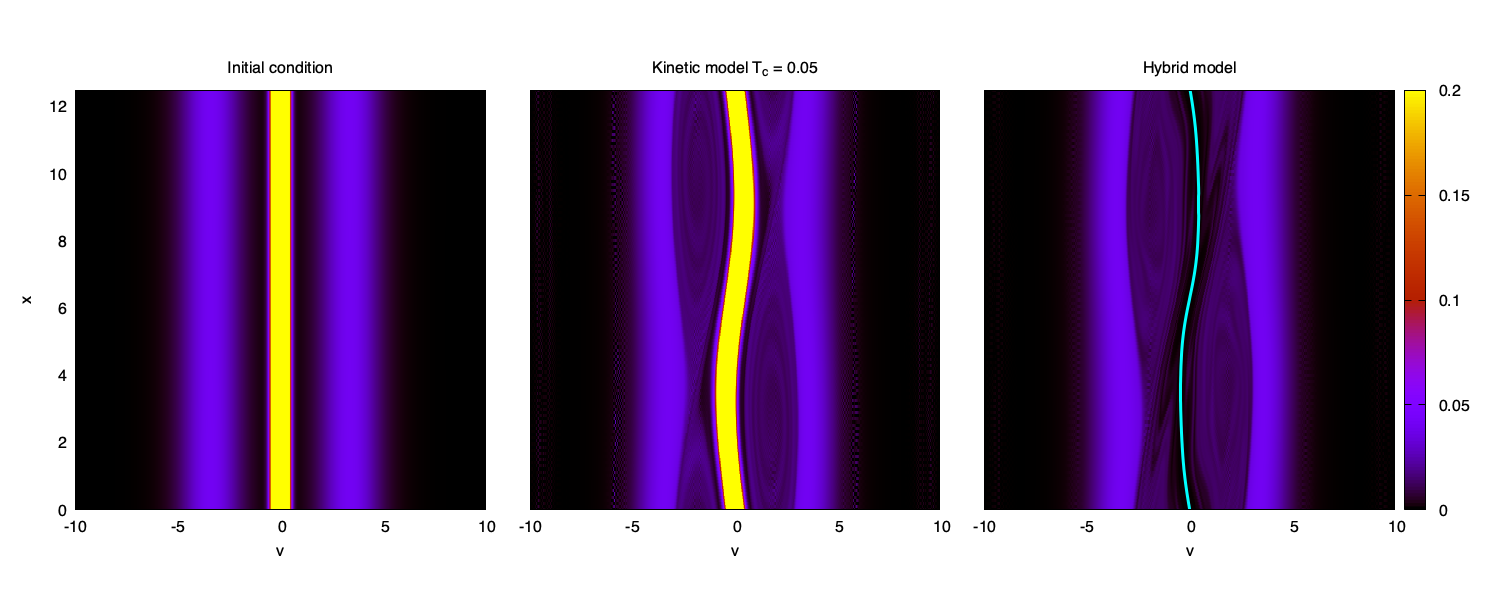
\includegraphics[width=\textwidth]{\localPath/figures/vp_t1.png}
  \caption{Représentation de la condition initiale du modèle cinétique à gauche et la solution obtenue au temps final $T_f=300$ avec le modèle cinétique avec $T_c = 0.05$ (au milieu) et la densité de particules chaudes obtenue avec modèle hybride linéarisé ainsi que la vitesse moyenne des particules froides (courbe cyan) (à droite).}
  \label{fig:limit_vp}
\end{figure}
\begin{figure}[h]
  \centering
  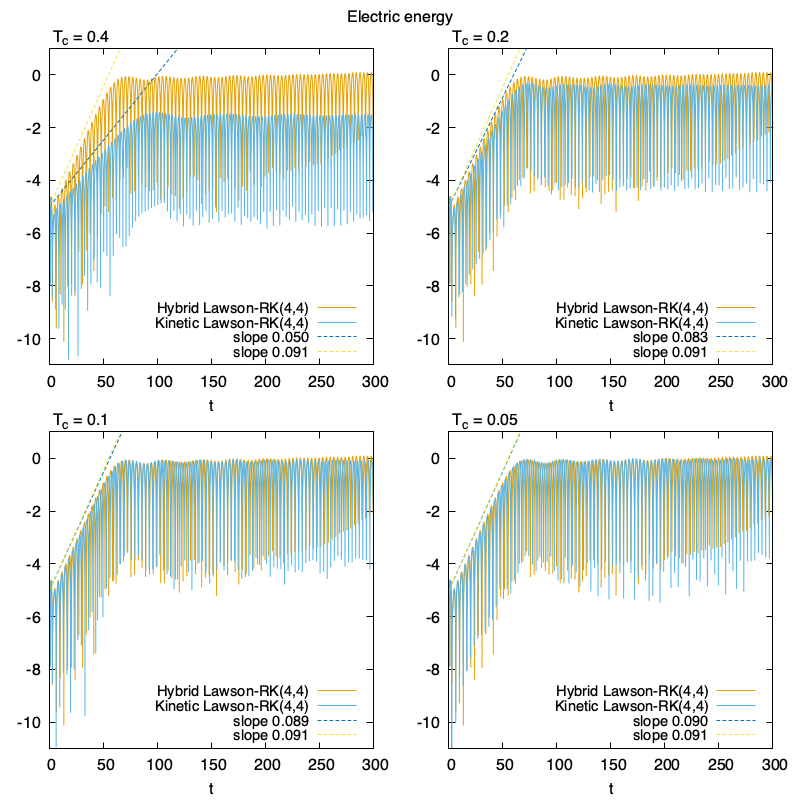
\includegraphics[width=\textwidth]{\localPath/figures/ee_t1.png}
  \caption{Énergie électrique donnée pour le modèle cinétique avec $T_c=0.05,0.1,0.2,0.4$ et le modèle hybride linéarisé.}
  \label{fig:limit_ee_Tf300}
\end{figure}
La première observation est que les résultats proches de ceux obtenus par le modèle hybride linéarisé \eqref{eq:vahl} sont très proches de ceux obtenus par le modèle cinétique \eqref{eq:vlasov}-\eqref{eq:poisson}, ce qui valide la modélisation. La perturbation des particules chaudes induit une instabilité (l'équilibre étant du type double gaussienne) qu'on voit se développer jusqu'au temps $t=75$ (voir figure \ref{fig:limit_ee_Tf300}), et deux vortex sont alors créés autour de la vitesse $v\approx 2$, au centre desquels de fines structures se développent. 

Dans la suite, nous allons approfondir cette étude en comparant les résultats obtenus aux relations de dispersion des deux modèles, puis en essayant de déterminer le domaine de validité du modèle VHL.  

%\commentaire[Anais]{(revoir un peu la rédaction de cette intro car elle ne tenait pas du tout compte de la sous-section relations de dispersion et je n'ai pas l'impression de l'avoir suffisamment modifiée)}

\FloatBarrier
%----------
\subsection{Convergence en énergie totale}
%----------

Nous nous intéresserons ici à une grandeur conservée qu'est l'énergie totale, celle-ci est la somme de l'énergie cinétique et de l'énergie électrique. Pour le modèle cinétique elle se calcule ainsi :
$$
  \mathcal{E}_K(t) = \iint_{\Omega\times\mathbb{R}} v^2 f\,\mathrm{d}x\mathrm{d}v + \int_{\Omega} E^2\,\mathrm{d}x. 
$$
Pour le modèle VHL, l'énergie cinétique comporte deux termes, un terme fluide pour les particules froides, et un terme cinétique pour les particules chaudes :
$$
  \mathcal{E}_{VHL}(t) = \int_\Omega \rho_c u_c^2\,\mathrm{d}x + \iint_{\Omega\times\mathbb{R}}v^2f_h\,\mathrm{d}x\mathrm{d}v + \int_\Omega E^2\,\mathrm{d}x
$$

\begin{pro}
  La différence en énergie totale entre le modèle cinétique et le modèle hybride linéarisé pour des conditions initiales données par~\eqref{eq:K:init} et~\eqref{eq:HL:init} converge en $(1-\alpha)T_c|\Omega|$.
\label{p:limit:convergence}
\end{pro}
\begin{proof}
  Pour le choix de $f^0$, l'énergie totale du modèle cinétique vaut :
  $$
    \begin{aligned}
      \mathcal{E}_K(t) = \mathcal{E}_K(0) &= \iint_{\Omega\times\mathbb{R}}v^2f^0(x,v)\,\mathrm{d}x\mathrm{d}v + \int_{\Omega}E^2(t=0,x)\,\mathrm{d}x \\
                                          &= \left[ (1-\alpha)T_c + \alpha v_0^2 + \alpha \right]|\Omega|
    \end{aligned}
  $$
    On remarque que lorsque $T_c\to 0$, on obtient $\lim_{T_c\to 0}\mathcal{E}_K(t) = (\alpha v_0^2 + \alpha)|\Omega|$. L'énergie totale dans le cadre du modèle hybride se calcule comme suit :
    $$
      \mathcal{E}_{HL}(t) = \int_\Omega \rho_c^{(0)}u_c^2\,\mathrm{d}x + \iint_{\Omega\times\mathbb{R}} v^2f_h\,\mathrm{d}x\mathrm{d}v + \int_\Omega E^2\,\mathrm{d}x
    $$
    ce qui nous donne, avec le choix de condition initiale $\rho_c^{(0)} = 1-\alpha$, $u_c^0 = 0$ et $f_h^0(v) = \mathcal{M}_{^\alpha/_2,v_0,1}(v) + \mathcal{M}_{^\alpha/_2,-v_0,1}(v)$, conformément à~\eqref{eq:HL:init} :
    $$
      \mathcal{E}_{HL}(t) = (\alpha v_0^2 + \alpha)|\Omega|
    $$
    qui est bien compatible avec $\lim_{T_c\to 0}\mathcal{E}_K(t)$. De plus on peut calculer :
    $$
      \mathcal{E}_K(t) - \mathcal{E}_{HL}(t) = (1-\alpha)T_c|\Omega|
    $$
    c'est-à-dire que la convergence du modèle hybride est liée à la pression $\rho_c^{(0)}T_c$ des particules froides.
\end{proof}

Pour vérifier numériquement cette proposition, nous effectuons un jeu de simulations. Le modèle cinétique de Vlasov-Poisson \eqref{eq:vlasov}-\eqref{eq:poisson} est simulé à l'aide d'une méthode en temps de type Lawson basée sur une méthode de Runge-Kutta d'ordre 4, la méthode WENO d'ordre 5 pour approcher la dérivée dans la direction $v$ et l'algorithme de FFT pour la dérivée dans la direction $x$. Il s'agit ainsi du même schéma que celui utilisé pour la fonction de distribution $f_h$ des particules chaudes du modèle hybride linéarisé. Nous choisissons la condition initiale \eqref{eq:K:init} avec $\alpha = 0.2$, $T_c \in \left\{ 0.05,0.1,0.2,0.4\right\}$, la discrétisation du domaine $\Omega = [0,4\pi]$ s'effectue avec $N_x = 135$ points, la discrétisation du domaine en vitesse $[-v_{\text{max}},v_{\text{max}}]$ nécessite de capturer la gaussienne représentant les particules froides pour différentes valeurs de $T_c$ ; nous choisissons donc d'adapter le nombre de points de discrétisation en vitesse $N_v$ à $T_c$, $N_v \in \left\{ 1431,1011,715,505 \right\}$, ceux-ci correspondant à une quinzaine de points de discrétisation pour capturer la gaussienne de température $T_c$. Nous avons une condition CFL sur le schéma WENO utilisé dans la direction $v$, nous nous assurons d'être sous cette condition quelle que soit l'évolution de $E$ en prenant $\Delta t = 0.5\Delta v$. Ce jeu de simulations s'arrête au temps 7, or le choix des différents $\Delta t$ implique des données à des temps différents ; nous choisissons d'effectuer une interpolation polynomiale de Lagrange d'ordre 5 pour exploiter les données au temps $T^\star = 6.5$. Nous obtenons ainsi l'énergie totale pour différentes températures sur la figure~\ref{fig:limit:totalenergy} ; bien que le schéma de type Runge-Kutta ne conserve pas exactement l'énergie, celle-ci est bien préservée en temps court et reste sous l'erreur machine en simple précision jusqu'au temps 50. Après l'interpolation au temps $T^\star = 6.5$ on obtient la convergence vers le modèle hybride sur la figure~\ref{fig:limit:totalenergy} (figure de droite) où l'on observe bien l'ordre 1 en température.
\begin{figure}[h]
  \centering
  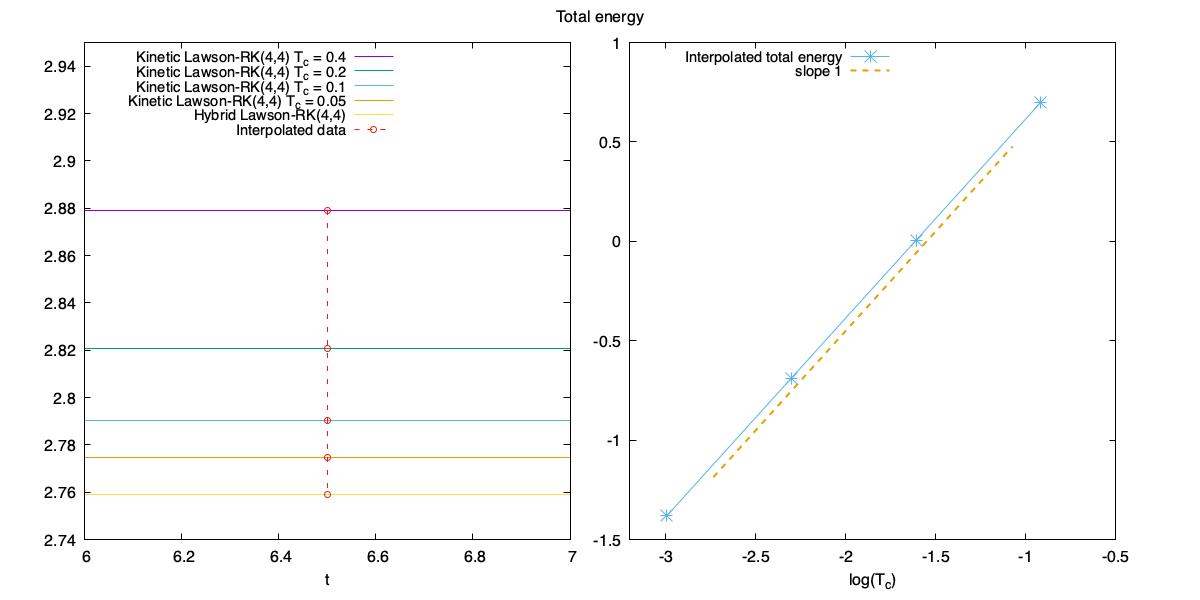
\includegraphics[width=\textwidth]{\localPath/figures/order_HTc.png}
  \caption{Énergie totale avec les différents modèles en échelle semi-log (gauche) et convergence de l'énergie totale du modèle cinétique vers le modèle hybride quand $T_c$ tend vers $0$ en échelle log (droite).}
  \label{fig:limit:totalenergy}
\end{figure}

Nous effectuons le même type d'analyse sur l'énergie électrique, à partir des données des simulations précédentes, en sachant que l'on n'a pas de résultat théorique sur sa convergence. L'énergie électrique pour les différents choix de $T_c$ est représentée sur la figure~\ref{fig:limit:ee} (gauche), cette figure illustre mieux la nécessité d'effectuer une interpolation pour extraire les données. Une convergence est observée sur la figure~\ref{fig:limit:ee} (droite).
\begin{figure}[h]
  \centering
  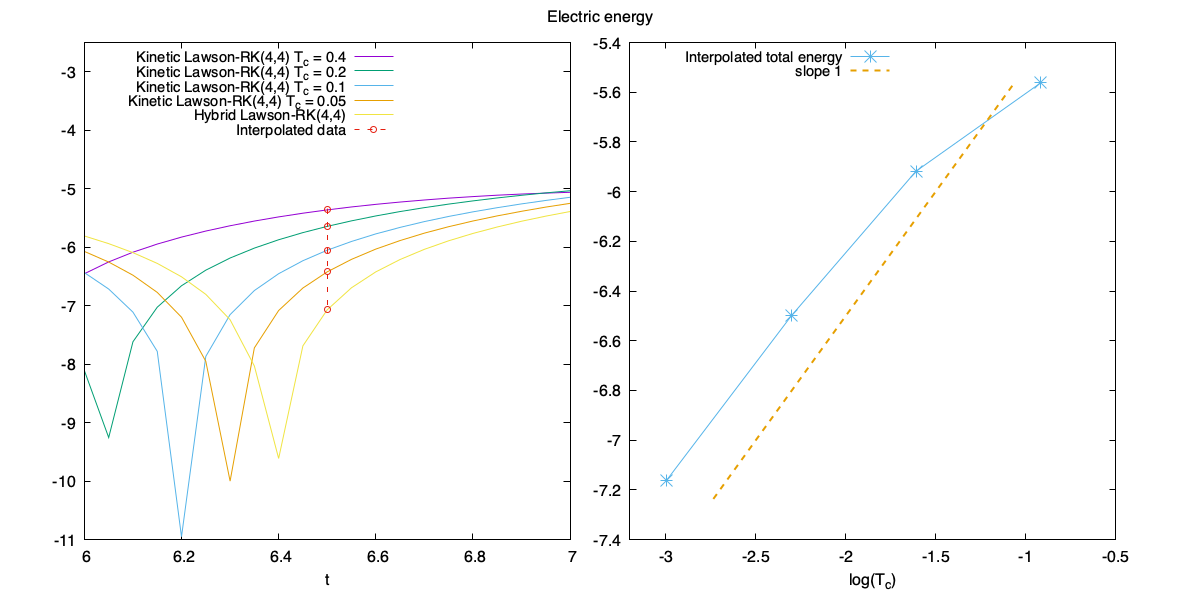
\includegraphics[width=\textwidth]{\localPath/figures/order_eeTc.png}
  \caption{Énergie électrique avec les différents modèles en échelle semi-log (gauche) et convergence de l'énergie totale du modèle cinétique vers le modèle hybride quand $T_c$ tend vers $0$ en échelle log (droite).}
  \label{fig:limit:ee}
\end{figure}

\FloatBarrier

%----------
\subsection{Convergence en température à l'aide des relations de dispersion}
%----------

Nous étudions numériquement la convergence des racines de la relation de dispersion quant $T_c$ tend vers $0$. Pour cela, on note $D^K_{[T_c]}(\omega,k)$ la relation de dispersion du modèle cinétique \eqref{D_3bump} et $D^H(\omega,k)$ la relation de dispersion du modèle VHL \eqref{eq:D_hchyb}. Pour $k$ fixé, on note $\omega\in\mathbb{C}$ la racine de plus grande partie imaginaire. 
%Pour la relation de dispersion, nous regardons les zéros en $\omega$ de la fonction $D^K_{[T_c]}(\omega,k)$ et $D^H(\omega,k)$ à $k$ fixé par la condition initiale. Nous ne conservons que le $\omega\in\mathbb{C}$ avec la plus grande partie imaginaire. 
Cette racine est calculée numériquement à l'aide d'une méthode de Newton. On étudie maintenant la convergence des $\omega_K$ (zéro de $(D^K(\omega,k)$) vers $\omega_H$ (zéro de $(D^H(\omega,k)$). La convergence de $\omega_K(T_c)$ vers $\omega_H$ est visible sur la figure \ref{fig:omega}, où l'on représente, en échelle log-log le module de la différence des deux zéros $\Delta \omega = |\omega_K-\omega_H|$.
\begin{figure}[h!]
  \centering
  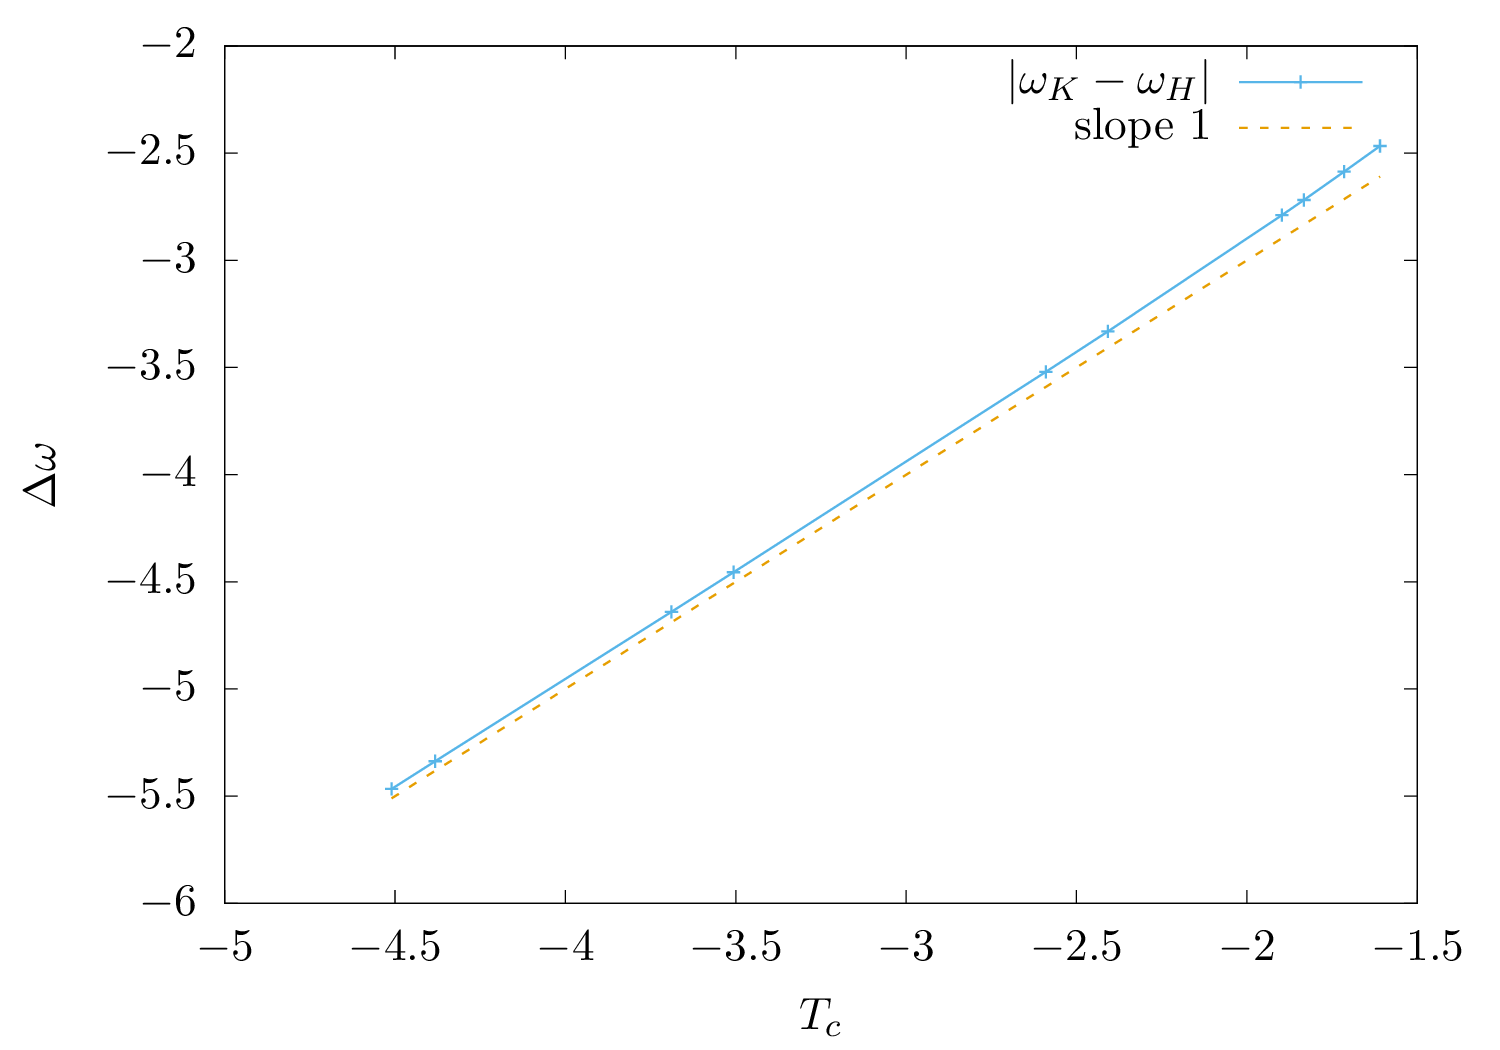
\includegraphics[width=0.8\textwidth]{\localPath/figures/omega.png}
  \caption{Convergence des zéros de la relation de dispersion cinétique vers la solution hybride}
  \label{fig:omega}
\end{figure}
On observe une convergence d'ordre $1$ en $T_c$ des zéros de la relation de dispersion, aucun argument théorique sur les fonctions holomorphes ne vient appuyer ce résultat, contrairement à ce qui a été énoncé pour l'énergie totale.

La racine de plus grande partie imaginaire permet de valider la phase linéaire du code. Cette phase linéaire peut être rendue plus longue en considérant une valeur très faible de la perturbation $\epsilon=10^{-4}$ dans les conditions initiales~\eqref{eq:K:init} et~\eqref{eq:HL:init}. Ceci va nous permettre de vérifier, non seulement le taux d'instabilité, mais aussi, grâce aux calculs de la section \ref{s:dispersion}, l'énergie électrique. Nous pouvons donc comparer pour $\alpha = 0.1$, $T_c=0.1$, $N_x=135$, $N_v=1200$, $T_f=200$ et $\Delta t = 0.5\Delta x$ ce régime linéaire sur la figure~\ref{fig:limit:ee:Tf200}\subref{fig:limit:ee:Tf200:eps10m4}. Un résultat similaire est observable pour différentes températures ainsi que sur le modèle hybride linéarisé, comme l'illustre la figure~\ref{fig:limit:ee:Tf200}\subref{fig:limit:ee:Tf200:cmp_zoom}. Les reconstructions de l'énergie électrique se font à partir des relations de dispersion, avec l'équation~\eqref{eq:enelec}.
\begin{figure}
  \centering
  \begin{subfigure}{0.8\textwidth}
    \centering
    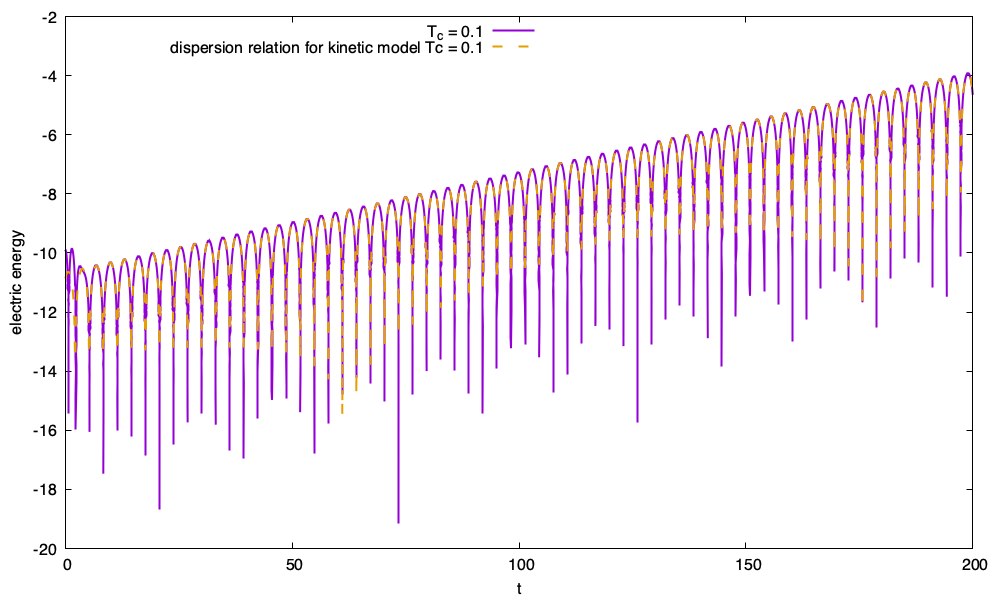
\includegraphics[width=\textwidth]{\localPath/figures/limit_ee_Tf200_eps10m4.png}
    \caption{Énergie électrique jusqu'au temps $200$ avec un régime linéaire très long, et comparaison avec les résultats données par les relations de dispersion.}
    \label{fig:limit:ee:Tf200:eps10m4}
  \end{subfigure}
  \begin{subfigure}{0.8\textwidth}
    \centering
    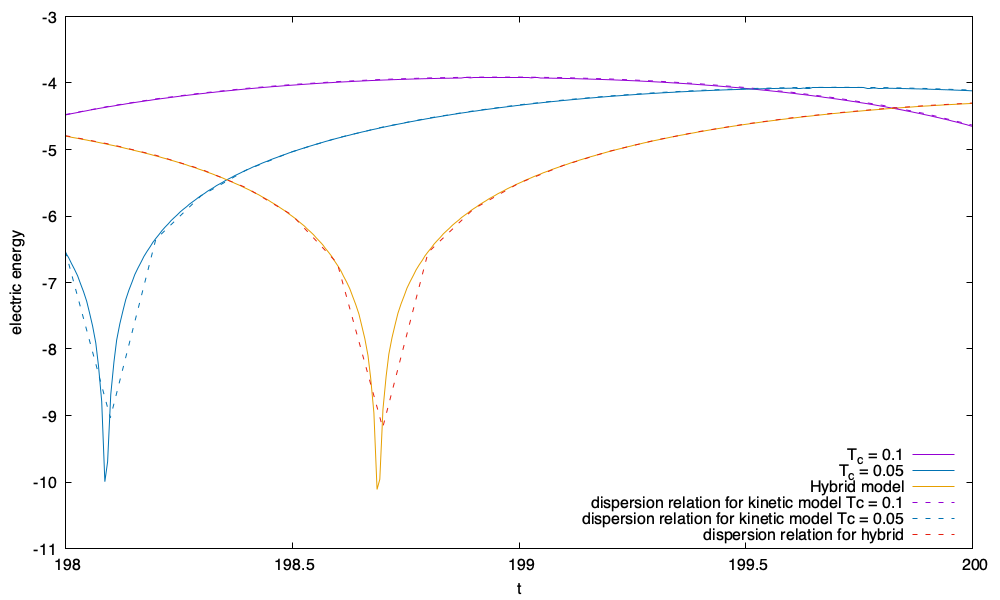
\includegraphics[width=\textwidth]{\localPath/figures/limit_ee_Tf200_cmp_zoom.png}
    \caption{Énergie électrique entre les temps $198$ et $200$ pour les températures $T_c = 0.1,0.05$ et le modèle hybride, et comparaison avec les résultats des relations de dispersion.}
    \label{fig:limit:ee:Tf200:cmp_zoom}
  \end{subfigure}
  \caption{Évolution de l'énergie électrique dans une longue phase linéaire et comparaison avec les relations de dispersion.}
  \label{fig:limit:ee:Tf200}
\end{figure}

En plus du taux d'instabilité de l'énergie électrique, il est possible, à l'aide des relations de dispersion, d'obtenir une très bonne approximation de l'énergie électrique dans la phase linéaire. On peut voir que l'étude des relations de dispersion ne permet pas d'obtenir des résultats fiables en début de simulation, où d'autres modes que le mode principal sont encore visibles (modes évanescents). De même, comme on peut le voir sur la figure~\ref{fig:limit_ee_Tf300}, la phase non-linéaire où l'énergie électrique atteint une saturation mélange de nombreux modes, ce qui est incompatible avec l'étude du linéarisé. Néanmoins, même au temps $t\approx 200$, les résultats du code sont en excellent accord avec ceux obtenus grâce aux relations de dispersion  (voir figure \ref{fig:limit:ee:Tf200:cmp_zoom}). 

\FloatBarrier
%----------
\subsection{Évolution avec la densité de particules chaudes}
%----------

Nous avons validé les modèles et les relations de dispersion lorsque la température des particules froides $T_c$ tend vers $0$ ; la proposition~\ref{p:limit:convergence} nous indique que la convergence s'effectue en $(1-\alpha)T_c|\Omega|$ où $\alpha$ est la densité des particules chaudes. Nous traçons sur la figure~\ref{fig:limit:slope:alpha} l'évolution du taux d'instabilité donné par les relations de dispersion (racine de plus grande partie imaginaire) en fonction de $\alpha$ et pour différentes valeurs de $T_c$. Cette évolution est représentée pour le modèle cinétique avec différentes températures, et  pour le modèle hybride, avec comme condition initiale pour les particules chaudes :
$$
  f_h^0(x,v) = \left(\mathcal{M}_{^\alpha/_2,4,1}(v) + \mathcal{M}_{^\alpha/_2,-4,1}(v)\right)(1+\epsilon\cos\left(k x\right)), \;\; x\in [0, 4\pi]. 
$$
La condition initiale du modèle cinétique est donnée par : $f^0(x,v) = \mathcal{M}_{1-\alpha,0,T_c}(v) + f_h^0(x,v)$.
\begin{figure}[h!]
  \centering
  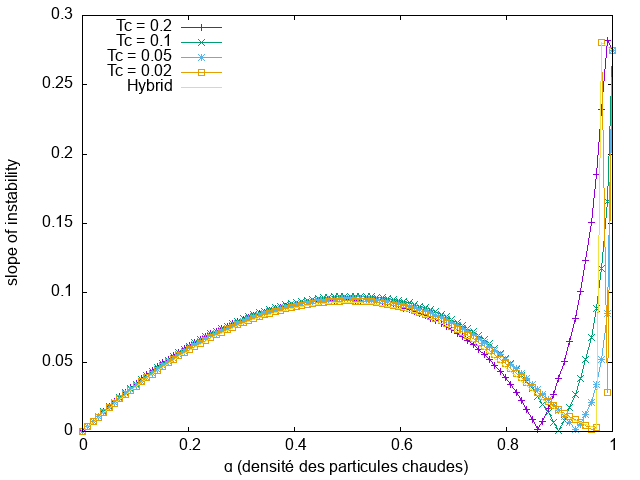
\includegraphics[width=0.8\textwidth]{\localPath/figures/limit_slope_alpha.png}
  \caption{Évolution de la pente du développement de l'instabilité (ou taux d'instabilité) donnée par les relations de dispersion en fonction de la densité de particules chaudes $\alpha$}
  \label{fig:limit:slope:alpha}
\end{figure}
On retrouve sur la figure~\ref{fig:limit:slope:alpha} la convergence en température du modèle cinétique vers le modèle hybride. Pour $\alpha=0$ la condition initiale se restreint aux particules froides, qui ne sont pas perturbées, il est donc normal d'obtenir une pente nulle ; pour $\alpha=1$, il n'y a que des particules chaudes et on retrouve l'instabilité double faisceau (TSI) avec le bon taux d'instabilité. On peut enfin observer que pour ce choix de $T_c$, les taux d'instabilité obtenus restent proches de ceux du modèle VHL pour $0\leq \alpha \leq 0.5$ (qui correspond à une population identique de particules chaudes et froides).

\FloatBarrier

%% section 7
% !TEX root = ../../main.tex

\section{Comparaison des deux résolutions hybrides}
\label{s:compare}

Dans cette section on s'intéressera à la comparaison des méthodes de simulation présentées dans la section~\ref{s:scheme} pour approcher numériquement le modèle VHL. On étudiera en particulier les méthodes de pas de temps adaptatif associées. Nous utilisons dans cette section la condition initiale suivante :
$$
  \begin{aligned}
    u_c(x)   &= 0 \\
    f_h(x,v) &=  \left(\mathcal{M}_{^\alpha/_2,v_0,1}(v) +  \mathcal{M}_{^\alpha/_2,-v_0,1}(v) \right)(1 + \epsilon\cos(kx))
  \end{aligned}
$$
avec $k=0.5$, $\alpha=0.2$, $v_0 = 3.4$, $x\in [0,L]$, $L=4\pi$, $v\in[-12,12]$, et la perturbation $\epsilon = 10^{-2}$. Le champ électrique initial $E(t=0,x)$ est obtenu en résolvant l'équation de Poisson sur notre condition initiale, comme indiqué dans la proposition~\ref{p:vhl_conservation}~:
$$
  \partial_x E(t=0) = (1-\alpha) + \int (1+\epsilon\cos(kx))\left( \mathcal{M}_{^\alpha/_2,v_0,1}(v) + \mathcal{M}_{^\alpha/_2,-v_0,1}(v) \right)\,\mathrm{d}v - 1
$$
La discrétisation du domaine s'effectue avec $N_x=27$ dans la direction $x$, et $N_v=128$ points dans la direction $v$.

Nous allons effectuer deux types de comparaisons entre les méthodes de \emph{splitting} hamiltonien et de Lawson. Une comparaison à pas de temps fixe, où on illustrera l'absence de condition de CFL des méthodes de \emph{splitting} ; puis une comparaison des méthodes de pas de temps adaptatif présentées dans la section~\ref{ssec:dtadapt} avec une tolérance $tol = 2\times10^{-5}$.

\subsection{Comparaison des deux résolutions hybrides à pas de temps fixe}

Cette section est dédiée à la comparaison entre la méthode de \emph{splitting} hamiltonien, présentée dans la sous-section~\ref{ssec:splitting}, et la méthode de Lawson présentée dans la sous-section~\ref{ssec:lawson}, pour la résolution du modèle hybride linéarisé~\eqref{eq:vahl}.

Nous considèrerons trois pas de temps différents :
\begin{itemize}
  \item $\Delta t = 0.1 \approx 0.5\Delta v$, il s'agit d'une condition de CFL classique pour des méthodes de volumes finis ;
  \item $\Delta t = 0.5 \approx \sigma\frac{\Delta v}{\|E^n\|_\infty} = 0.54$, with $\sigma\approx 1.732$, il s'agit de la condition de CFL entre WENO5 et RK($4$,$4$) calculé dans le chapitre précédent ou~\cite{Crouseilles:2019b}, et calculé à partir d'une précédente estimation numérique $\|E^n\|_\infty = \max_{i,n}|E^n_i|\approx 0.6$ ;
  \item $\Delta t = 0.7$, il s'agit dans ce cas d'un cas test avec un pas de temps plus grand que la CFL de la méthode de Lawson, pour illustrer que la méthode de \emph{splitting} n'a pas de contrainte de stabilité sur le pas de temps.
\end{itemize}

Sur la figure~\ref{fig:compare:ee}, on trace l'évolution de l'énergie électrique (en échelle semi-log) calculée par deux méthodes d'ordre 4 (méthode de Suzuki et de Lawson-RK(4,4)), avec différentes valeurs de pas de temps $\Delta t$, $0.1$, $0.5$ et $0.7$. On note que toutes les simulations capturent correctement l'énergie électrique dans la phase linéaire, jusqu'au temps 60, même lorsque la méthode est instable. Pour $\Delta t=0.1,0.5$, on vérifie la stabilité prévue des méthodes, qui donnent des résultats très similaires. Dans le cas $\Delta t=0.7$, la méthode de Lawson-RK(4,4) devient instable dans la phase non-linéaire, c'est en fait dans cette phase que l'amplitude du champ électrique atteint son maximum, et le paramètre $\Delta t=0.7$ viole la condition de CFL, alors que la méthode de \emph{splitting} de Suzuki reste stable comme prévu.

\begin{figure}[h]
  \centering
  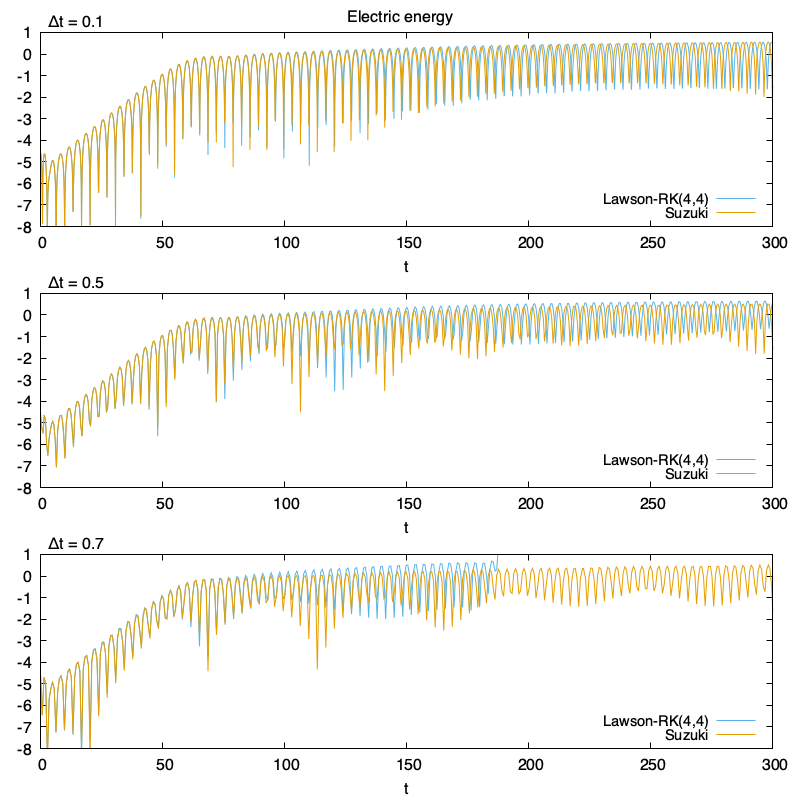
\includegraphics[width=\textwidth]{\localPath/figures/ee_t2.png}
  \caption{Évolution de l'énergie électrique pour le modèle hybride (résolu avec la méthode de Lawson et de Suzuki) pour différentes valeurs de pas de temps $\Delta t=0.1,0.5,0.7$.}
  \label{fig:compare:ee}
\end{figure}


Sur la figure~\ref{fig:H:t2}, on observe l'évolution de l'erreur relative sur l'énergie totale, calculée par :
\begin{equation}
	\frac{\mathcal{H}^n}{\mathcal{H}^0}-1
	\label{eq:relativeerror:H}
\end{equation}
avec :
$$
  \mathcal{H}^n = \frac{1}{2}\iint v^2f_h^n\dd{v}\dd{x}
                + \frac{1}{2}\int\rho_c^{(0)}\left(u_c^n\right)^2\dd{x}
                + \frac{1}{2}\int\left(E^n\right)^2\dd{x}.
$$
On considère les mêmes paramètres numériques et on compare l'effet de la méthode d'intégration en temps (méthode de \emph{splitting} hamiltonien : Lie~\eqref{eq:lie}, Strang~\eqref{eq:strang} et Suzuki~\eqref{eq:suzuki}, et la méthode Lawson-RK(4,4)) sur la préservation de l'énergie totale. On observe que les méthodes géométriques de \emph{splitting} hamiltonien préservent très bien l'énergie totale, en particulier, l'erreur relative oscille autour d'une constante en temps long, ce qui est un comportement typique d'une méthode géométrique. On observe que la méthode de Lawson, si le pas de temps est pris sous la condition de CFL, l'erreur est proche de $4\%$, ce qui est acceptable. Évidemment, comme évoqué précédemment sur l'énergie électrique, on observe un problème lorsque $\Delta t=0.7$, l'erreur donnée par la méthode Lawson-RK($4$,$4$) diverge dans la phase non-linéaire, à cause de l'instabilité numérique ; avant cela, l'erreur est autour des $2\%$. Le tableau~\ref{tab:H:max} résume le maximum de l'erreur relative $\max_n \left| {\cal H}^n / {\cal H}^0 -1 \right|$ pour les différentes méthodes et les différents pas de temps considérés.

\begin{figure}[h]
  \centering
  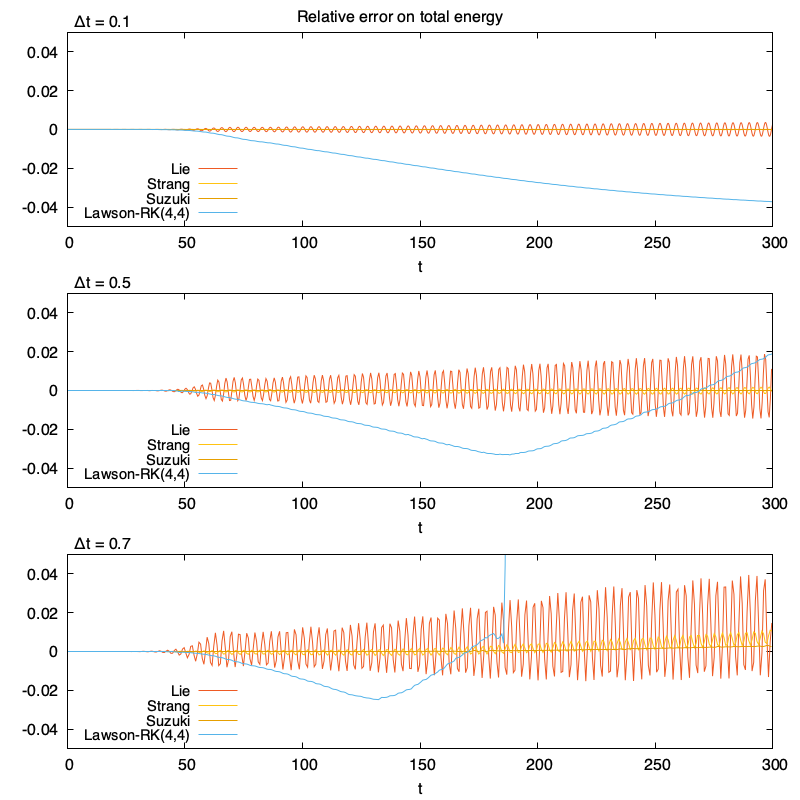
\includegraphics[width=\textwidth]{\localPath/figures/H_t2.png}
  \caption{Évolution de l'erreur relative sur l'énergie totale pour le modèle hybride (résolu avec la méthode de Lawson et de Suzuki) pour différentes valeurs de pas de temps $\Delta t=0.1,0.5,0.7$.}
  \label{fig:H:t2}
\end{figure}

\begin{table}[h]
  \centering
  \begin{tabular}{l|c|c|c}
                   & $0.1$             & $0.5$     & $0.7$        \\
    \hline
    Lie            & $0.0036$          & $0.0187$  & $0.0394$     \\
    Strang         & $0.0001$          & $0.0019$  & $0.0109$     \\
    Suzuki         & $3\times 10^{-8}$ & $0.0001$  & $0.0028$     \\
    Lawson-RK(4,4) & $0.0372$          & $0.0331$  & \texttt{NaN} \\
  \end{tabular}
  \caption{Maximum de l'erreur relative donnée sur la figure~\ref{fig:H:t2}.}
  \label{tab:H:max}
\end{table}

Dans le cas $\Delta t=0.1$, on compare sur la figure~\ref{fig:vp:t2} la distribution de particules chaudes $f_h$ calculée par les méthodes de Suzuki et de Lawson-RK(4,4) au temps $t=100$, sur laquelle on ajoute la vitesse moyenne des particules froides $u_c$. Les solutions numériques ainsi obtenues sont très proches, la position des vortex et l'allure de la vitesse moyenne des particules froides sont très similaires entre les deux méthodes. On observe aussi que la méthode Lawson-RK(4,4) introduit plus de diffusion numérique que la méthode de Suzuki, en effet les vortex semblent avoir une meilleure résolution. Cela peut s'expliquer par la discrétisation dans l'espace des phases dans la direction $v$, une méthode WENO5 (avec limiteurs de pente) est utilisé avec la méthode Lawson-RK(4,4), contre une interpolation d'ordre 5 par des polynômes de Lagrange (sans limiteurs de pente) avec la méthode de Suzuki.

\begin{figure}[h]
  \centering
  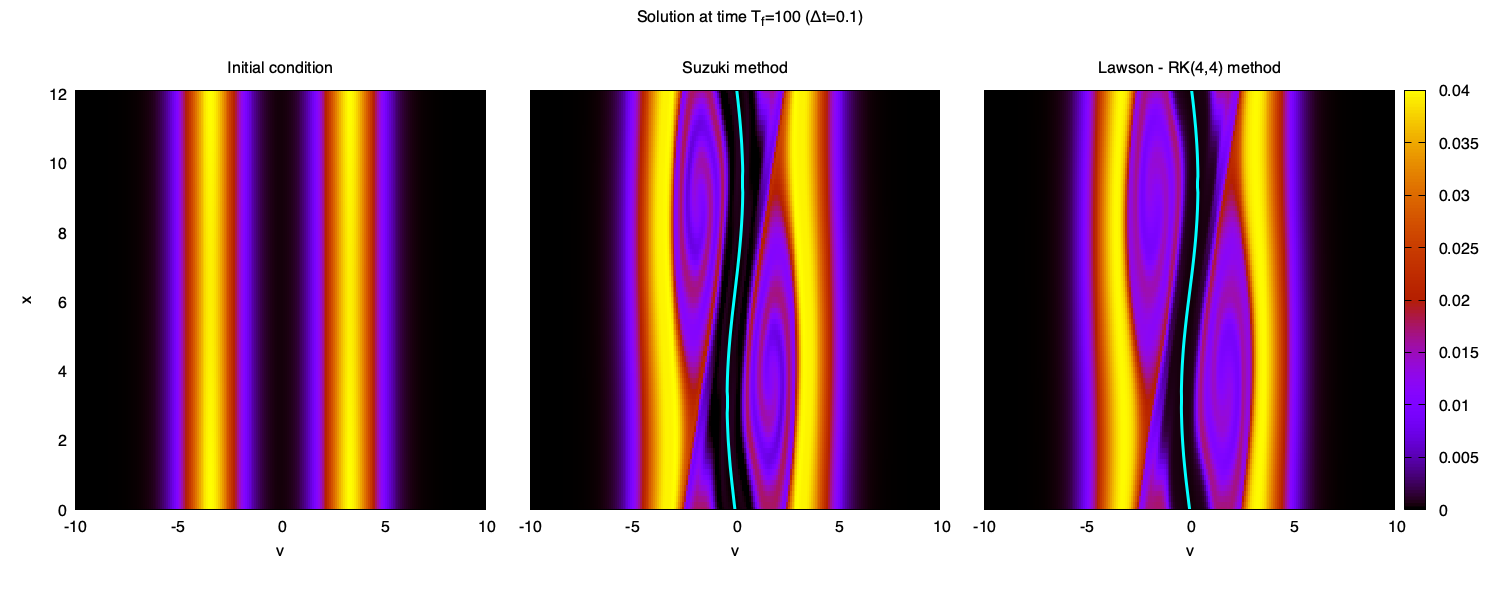
\includegraphics[width=0.9\textwidth]{\localPath/figures/vp_t2.png}
  \caption{Densité des particules chaudes $f_h$ et vitesse moyenne des particules froides $u_c$ (en cyan) la condition initiale (gauche), au temps $t=100$ calculée par la méthode de Suzuki (milieu) et calculée par la méthode de Lawson-RK(4,4) (droite).}
  \label{fig:vp:t2}
\end{figure}

\begin{figure}
	\centering
	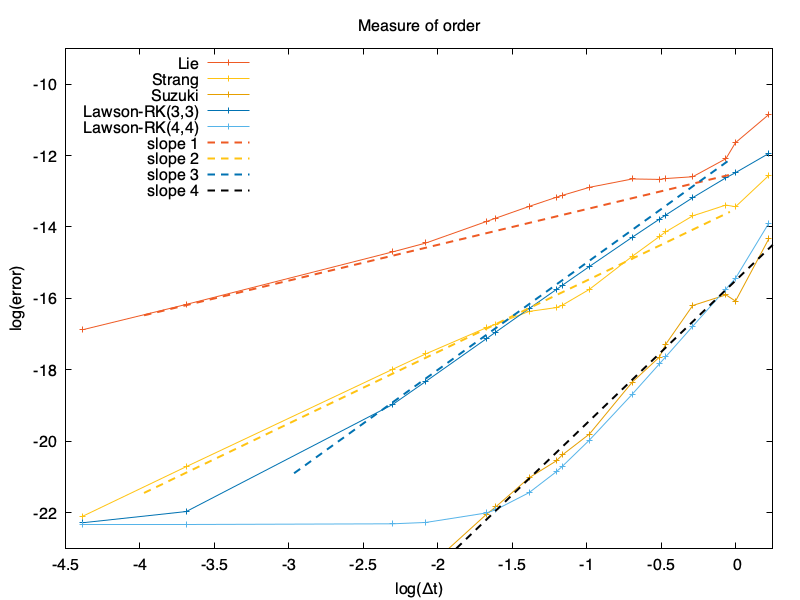
\includegraphics[width=0.75\textwidth]{\localPath/figures/order_t2.png}
	\caption{Étude de l'ordre en temps des différentes méthodes numériques pour résoudre le modèle hybride (méthodes de Lawson et de \emph{splitting}). L'erreur est calculée à partir du maximum de l'erreur relative sur l'énergie totale.}
	\label{fig:order:t2}
\end{figure}

Pour compléter cette étude, on trace sur la figure~\ref{fig:order:t2} l'ordre en temps des différents intégrateurs en temps utilisés pour résoudre le modèle hybride : les méthodes de \emph{splitting} hamiltonien (Lie, Strang et Suzuki), les méthodes de Lawson (RK(4,4) et RK(3,3)). Pour cela on calcule le maximum de l'erreur relative sur l'énergie totale : $\max_n|\mathcal{H}^n/\mathcal{H}^0-1|$, jusqu'au temps $t=15$, en fonction du pas de temps $\Delta t\in[0.01,0.125]$, avec $N_x=243$ et $N_v=512$. Tous les ordres théoriques des méthodes en temps sont bien reconstruits. On remarque que la constante d'erreur entre la méthode de Suzuki et de Lawson-RK(4,4) sont très proches, mais que cette première est légèrement plus coûteuse que la méthode de Lawson (plus de détails dans la section~\ref{ssec:2:time}).

\FloatBarrier

\subsection{Comparaison des deux méthodes de pas de temps adaptatif}
\label{ssec:2:dtn}

Cette section est dédiée à l'étude des méthodes de Suzuki et de Lawson avec leur stratégie de pas de temps adaptatif associée, présentée dans la section~\ref{ssec:dtadapt}. Pour toutes les simulations nous nous somme intéressés à l'estimateur d'erreur qui dans ce cas s'écrit :
\begin{equation}
  \begin{aligned}
    L^{n+1}_{[3]} & = \left(\sum_{i=0}^{N_x-1}\left( {u_c}_i^{n_1,[4]}-{u_c}_i^{n_1,[3]} \right)^2\Delta x\right)^{\frac{1}{2}}
                    + \left(\sum_{i=0}^{N_x-1}\left( {E}_i^{n_1,[4]}-{E}_i^{n_1,[3]} \right)^2\Delta x\right)^{\frac{1}{2}} \\
                  & + \left(\sum_{i=0}^{N_x-1}\sum_{j=0}^{N_v-1}\left| {f_h}_{i,j}^{n_1,[4]}-{f_h}_{i,j}^{n_1,[3]} \right|^2\Delta v\Delta x\right)^{\frac{1}{2}} \\
                  & = L_{u_c}^{n+1} + L_{E}^{n+1} + L_{f_h}^{n+1},
  \end{aligned}
  \label{eq:LucEfh:localerror}
\end{equation}
où ${u_c}_i^{n+1,[p]}$,${E}_i^{n+1,[p]}$ et ${f_h}_{i,j}^{n+1,[p]}$ sont les inconnues discrétisées calculées avec une méthode d'ordre $p$ en temps et associées au temps $t^{n+1}$ et au point $x_i=i\Delta x$, $i=0,\dots,N_x$ et $v_j = -v_\text{max} + j\Delta v$, $j=0,\dots,N_v$ de l'espace des phases. Pour les deux méthodes, si le critère d'erreur $\|L_{[3]}^{n+1}\|<tol$ est satisfait, alors l'itération est acceptée et le temps incrémenté, sinon l'itération est rejetée et reprend au temps $t^n$. Dans les deux cas, le pas de temps suivant est calculé en utilisant~\eqref{eq:dtopt}. Cela nous permet de comparer l'estimateur d'erreur avec la même tolérance $tol$ (prise arbitrairement à $tol=2\times10^{-5}$) entre les deux intégrateurs en temps : la méthode de Suzuki et DP4(3). Nous regarderons aussi la taille des pas de temps proposés par les deux méthodes et le nombre d'itérations nécessaires pour finir la simulation.

\begin{table}[h]
	\centering
	\begin{tabular}{c|c|c|c}
      méthode             & nombre d'itérations & nombre d'itérations acceptées & ratio \\
%      \hline
%       $\Delta t = 0.5$ & 600                  & 600                          & 1     \\
%       $\Delta t = 0.1$ & 3000                 & 3000                         & 1     \\
      \hline
      Suzuki              & 23895                & 23849                        & 0.998 \\
      Lawson-DP4(3)       & 2288                 & 2192                         & 0.958 \\
	\end{tabular}
	\caption{Comparaison du nombre d'itérations pour résoudre le problème jusqu'au temps $t=300$, le nombre d'itérations acceptées de la méthode de pas de temps adaptatif et le ratio entre le nombre d'itérations acceptées et le nombre total d'itérations.}
	\label{tab:compare:iteration}
\end{table}

Le tableau~\ref{tab:compare:iteration} présente le nombre d'itérations nécessaires pour atteindre le temps final $t=300$ pour les deux méthodes de pas de temps adaptatif considérées (méthode de Suzuki et de Lawson-DP4(3)) avec les paramètres numériques suivants $N_x=81$, $N_v=128$. Le nombre d'itérations acceptées (itérations où le critère d'erreur $\|L_{[3]}^{n+1}\|<tol$ est satisfait), et le ratio entre le nombre d'itérations acceptées et le nombre total d'itérations est aussi présenté. On observe qu'une très large majorité des itérations sont acceptées pour les deux méthodes, ce qui signifie que l'estimateur d'erreur est un bon indicateur. Pour la méthode de Lawson-DP4(3) le ratio d'itérations acceptées est légèrement plus faible que pour la méthode de Suzuki, ce qui signifie que la stratégie de pas de temps adaptatif essaie des pas de temps plus larges qui sont parfois rejetés. La très faible proportion d'itérations rejetées indique qu'il est très rarement nécessaire de recalculer une itération avec un pas de temps plus petit. Le surcoût engendré par la méthode de pas de temps adaptatif est donc négligeable. La seconde remarque que l'on peut faire est à propos de la méthode de Suzuki, qui nécessite 10 fois plus d'itérations que la méthode de Lawson-DP4(3) pour atteindre le temps final $t=300$, ce qui signifie que la méthode de Suzuki nécessite de plus petits pas de temps pour satisfaire le critère d'erreur $\|L_{[3]}^{n+1}\|<tol$.

Sur la figure~\ref{fig:compare:dt_and_error} est représentée l'évolution de la taille du pas de temps au cours du temps, en effet celui-ci suit l'équation~\eqref{eq:dtopt} et est donc recalculé à chaque itération. Les itérations rejetées, celles où le critère d'erreur n'est pas satisfait, sont représentées avec des carrés. On remarque tout d'abord que dans la phase linéaire (jusqu'au temps $t\approx 50$) des pas de temps plus grands sont pris. Pendant la phase non-linéaire, le pas de temps oscille près d'une constante, qui permet de capturer les effets non-linéaires (vortex dans la distribution de particules) et les forts gradients (filamentation issue de la formation des votex). On remarque ensuite, que pour une même tolérance ($tol=2\times10^{-5}$), la méthode de Suzuki nécessite de plus petits pas de temps, comparé à la méthode DP4(3), pour satisfaire le critère d'erreur, comme remarqué dans le tableau~\ref{tab:compare:iteration}. On remarque que les variations du pas de temps sont relativement importantes ; il est possible de contrôler ces oscillations en limitant l'évolution des pas de temps en prenant par exemple $\Delta t^{n+1}\in[0.5\Delta t^n,2\Delta t^n]$, comme proposé dans \cite{Balac:2014}. Sur la figure~\ref{fig:compare:error:dtc} est tracée l'évolution de l'erreur locale $L_{[3]}^n$ comme une fonction du temps pour la méthode de Lawson (gauche) et de Suzuki (droite), avec une stratégie de pas de temps adaptatif et une stratégie de pas de temps constant. Pour un grand pas de temps ($\Delta t = 0.5$), les méthodes sont stables, mais le pas de temps dépasse largement la tolérance fixée à $tol=2\times10^{-5}$. Les méthodes à pas de temps adaptatif, choisissent automatiquement un pas de temps permettant de garantir une erreur locale sous la tolérance. La méthode de Lawson avec un pas de temps adaptatif (DP4(3)) et avec un pas de temps fixe à $\Delta t = 0.1$ (RK(4,4)) calculent une erreur locale très proche, pourtant la méthode DP4(3) optimise son pas de temps pour assurer une erreur locale sous la tolérance, et permet d'obtenir des pas de temps plus grand que $\Delta t =0.1$ comme on peut le remarquer sur la figure~\ref{fig:compare:dt_and_error}. Assurer une erreur sous une tolérance avec les plus grands pas de temps possible est une heuristique intéressante. En ce qui concerne les résultats avec la méthode de Suzuki, on remarque de nouveau que la stratégie requière de plus petits pas de temps, comparé à DP4(3), pour assurer une estimation de l'erreur locale sous la tolérance. De plus, avec un pas de temps constant à $\Delta t = 0.1$, la méthode de Suzuki génère des erreurs locales bien plus importantes, alors que la méthode DP4(3) était presque sous la tolérance.

\begin{figure}[h]
  \centering
  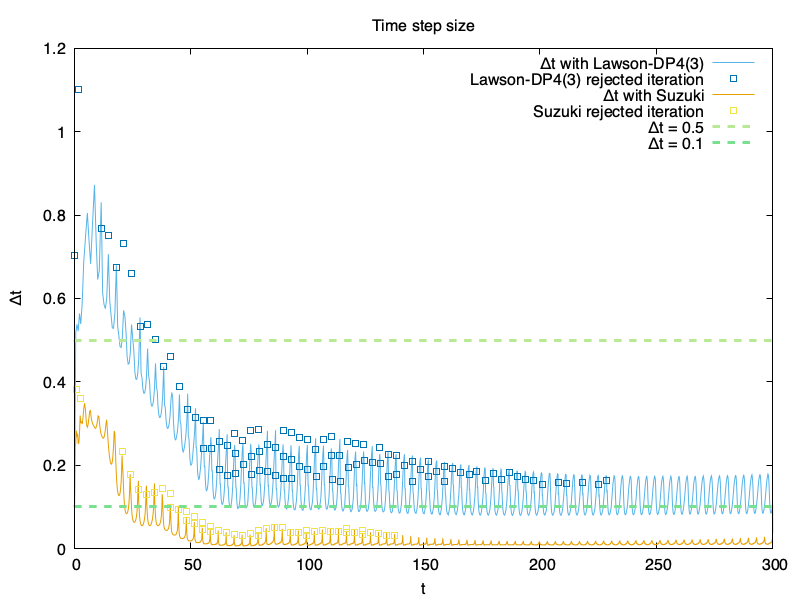
\includegraphics[width=0.75\textwidth]{\localPath/figures/dt_size_t3.png}
  \caption{Évolution du pas de temps $\Delta t_n$ (les itérations rejetées sont représentées par des carrés) pour la modèle hybride avec des méthodes de pas de temps adaptatif.} 
  \label{fig:compare:dt_and_error}
\end{figure}

\begin{figure}[h]
  \centering
  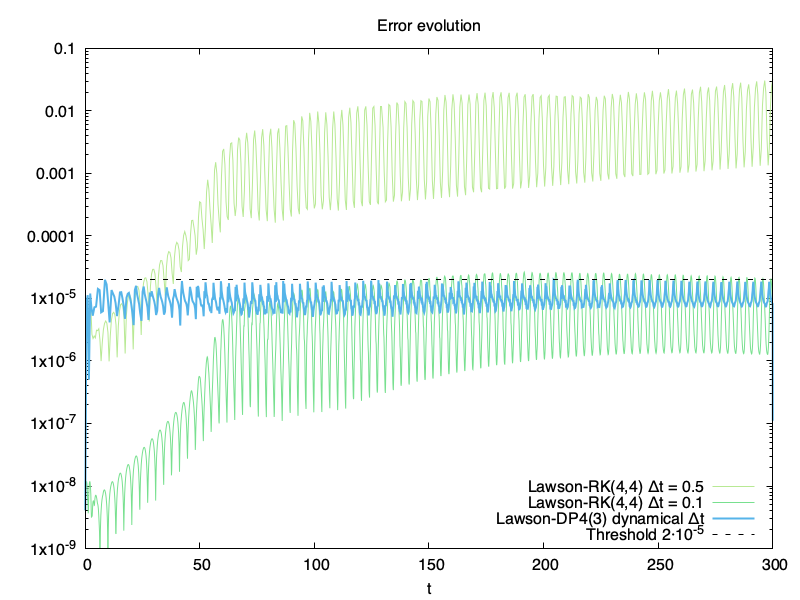
\includegraphics[width=0.49\textwidth]{\localPath/figures/Ll_t3.png}
  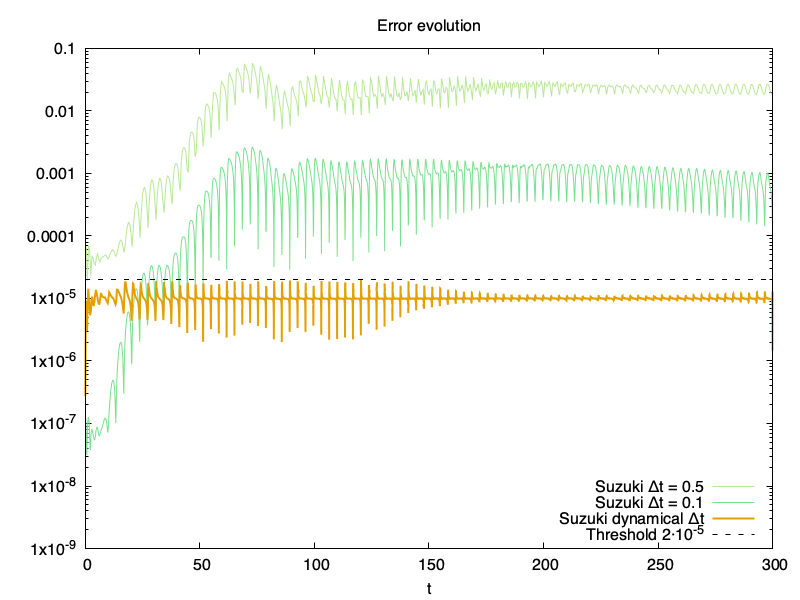
\includegraphics[width=0.49\textwidth]{\localPath/figures/Ls_t3.png}
  \caption{Comparaison de l'évolution en temps de l'estimateur d'erreur pour une méthode à pas de temps constant et à pas de temps adaptatif. La méthode de Lawson est à gauche. La méthode de Suzuki est à droite. Les résultats sont en échelle semi-$\log$.}
  \label{fig:compare:error:dtc}
\end{figure}
\begin{figure}[h]
  \centering
  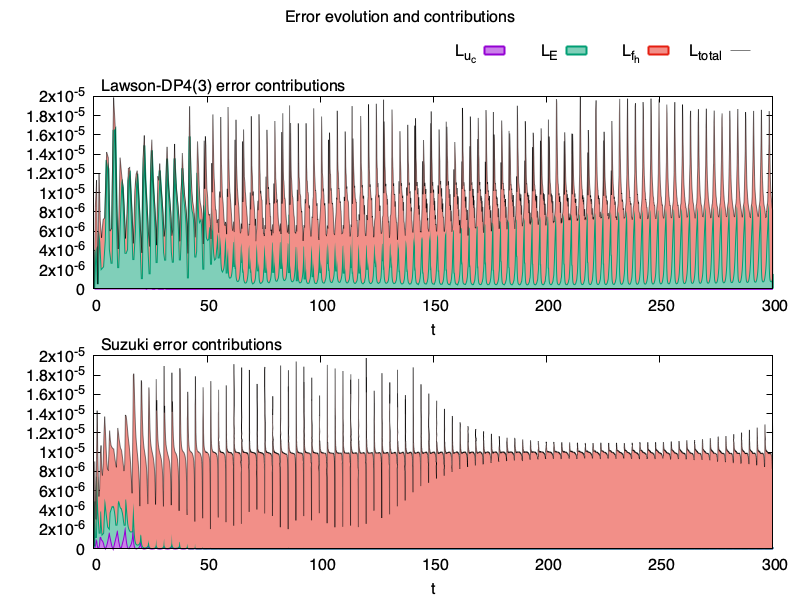
\includegraphics[width=0.8\textwidth]{\localPath/figures/L_LucEfh_t3.png}
  \caption{Comparaison de la contribution de chaque composante de l'estimateur d'erreur locale en fonction du temps, pour la méthode de Lawson (haut) et de Suzuki (bas).}
  \label{fig:compare:error:LucEfh}
\end{figure}

Pour les deux méthodes à pas de temps adaptatif, on s'intéresse maintenant à l'évolution de l'estimateur d'erreur locale au cours du temps, en prennant en compte les différentes contributions de $L^n_{[3]}$, à savoir $L^n_{u_c}$, $L^n_{E}$ et $L^n_{f_h}$ définies dans~\eqref{eq:LucEfh:localerror}. Les résultats sont visibles sur la figure~\ref{fig:compare:error:LucEfh}. L'erreur de la méthode DP4(3) et de ces différentes contributions sont visibles en haut, alors que celles de la méthode de Suzuki sont tracées en bas. Pour la méthode DP4(3), on remarque tout d'abord que la contribution venant de $L^n_{u_c}$ est négligeable (autour de l'erreur machine), ce qui peut s'expliquer par le fait que dans la méthode de Lawson la partie linéaire est résolue exactement. Puisque la partie non-linéaire de la méthode de Lawson comprend le calcul du courant chaud $\int vf_h\dd{v}$ qui va impacter $L^n_E$ et le transport dans la direction $v$ qui va impacter $L^n_{f_h}$, les contributions à l'estimateur d'erreur de ces deux contributions restent prépondérantes tout au long de la simulation. Pour la méthode de Suzuki, l'erreur provient essentiellement de $L^n_{f_h}$, erreur venant de l'interpolation du transport dans la direction $v$. Il est à noter, que les erreurs $L^n_{u_c}$, $L^n_{E}$ ne sont pas nulles au delà du temps $t\approx 50$, mais sont respectivement de l'ordre de $10^{-10}$ et $10^{-8}$.

%\FloatBarrier

\subsection{À propos des temps de calcul}
\label{ssec:2:time}

Pour finir la comparaison entre les méthodes de \emph{splitting} et de Lawson, nous comparerons leurs temps de calcul. Sur la figure~\ref{fig:timer_boxplot_t4} (gauche), on représente la valeur moyenne ainsi que les quartiles du temps de calcul d'une itération de RK(4,4), DP4(3) et de la méthode de Suzuki. Nous rappelons que la méthode RK(4,4) est constituée de 4 étages, alors que les méthodes DP4(3) et de Suzuki en comprennent 5. Cela explique pourquoi une itération de la méthode RK(4,4) coûte moins qu'une itération des deux autres méthodes. Sur la partie de droite de la figure~\ref{fig:timer_boxplot_t4} on compare le temps de calcul de chaque étape des différentes méthodes. On rappelle que la méthode DP4(3) est formée à partir des 4 étages de la méthode RK(4,4) plus un étage supplémentaire. Comme espéré, chaque étape de la méthode de Suzuki a le même coût (puisque la méthode de Suzuki est une composition de 5 méthode de Strang). Au contraire, on observe que les deux premiers étages des méthodes RK(4,4) ou DP4(3) sont moins coûteux que les autres étages, ces deux premiers contenant moins d'opérations.

\begin{figure}[h]
  \centering
  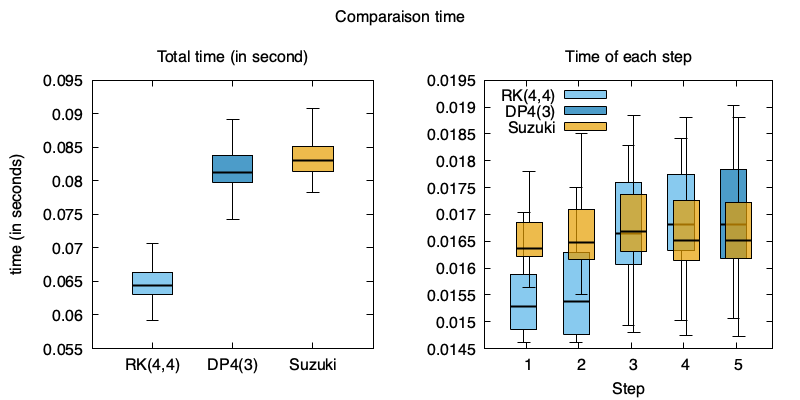
\includegraphics[width=\textwidth]{\localPath/figures/timer_boxplot_t4.png}
  \caption{Valeur moyenne et quartiles du temps de calcul sur une itération (gauche) et pour chaque étape d'une itération (droite).}
  \label{fig:timer_boxplot_t4}
\end{figure}


% annexe
\begin{subappendices}
% !TEX root = ../chap2.tex

\section{Résultats sur les relations de dispersion}
\label{a:dispersion}

Cette annexe est dédiée aux démonstrations des propriétés énoncées dans la section \ref{s:dispersion} sur les relations de dispersion.

Nous démontrons tout d'abord le lemme \ref{lemma:doubleracine}, qui concerne la symétrie des racines de $D(k,\omega)$, et dont l'énoncé est rappelé ci-dessous.
\begin{lemma}
  Si $f^{(0)}(v)$ (respectivement $f_h^{(0)}(v)$) est une fonction paire, alors pour $D(k,\omega)$ défini par (\ref{eq:D}) (respectivement (\ref{eq:relD_H})) nous avons $D(k,\omega_r+i\omega_i) = 0 \Leftrightarrow D(k,-\omega_r+i\omega_i)=0$.
\end{lemma}

\begin{proof}
  Nous le vérifions dans le cas cinétique, les calculs étant similaires dans le cas hybride. Avec la définition (\ref{eq:D}) de $D(k,\omega)$, nous avons 
  \begin{eqnarray*}
    &&D(k,\omega_r+i\omega_i)=0\\
    &\Leftrightarrow&
    \Re\left(\frac{1}{k^2}\int_\gamma\frac{\partial_vf^0}{v-\frac{\omega_r+i\omega_i}{k}}dv\right)=1,~\Im\left(\frac{1}{k^2}\int_\gamma\frac{\partial_vf^0}{v-\frac{\omega_r+i\omega_i}{k}}dv\right)=0. 
  \end{eqnarray*}
  Distinguons les parties réelles et imaginaires :
  \begin{eqnarray*}
    \int_\gamma\frac{\partial_vf^0(v)}{v-\frac{\omega_r+i\omega_i}{k}}dv=\int_\gamma\frac{\partial_vf^0(v)}{\left(v-\frac{\omega_r+i\omega_i}{k}\right)\left(v-\frac{\omega_r-i\omega_i}{k}\right)}\left(v-\frac{\omega_r-i\omega_i}{k}\right)dv\\
    =\int_\gamma\frac{\partial_vf^0(v)}{\left(v-\frac{\omega_r}{k}\right)^2+\left(\frac{\omega_i}{k}\right)^2}\left(v-\frac{\omega_r}{k}\right)dv+i\int_\gamma\frac{\partial_vf^0(v)}{\left(v-\frac{\omega_r}{k}\right)^2+\left(\frac{\omega_i}{k}\right)^2}\frac{\omega_i}{k}dv.
  \end{eqnarray*}
  Maintenant, considérons $\omega=-\omega_r+i\omega_i$ et rappelons qu'on a supposé que $f^0(v)$ était une fonction paire. Nous obtenons
  \begin{eqnarray*}
    \int_\gamma\frac{\partial_vf^0(v)}{v-\frac{-\omega_r+i\omega_i}{k}}dv~~~~~~~~~~~~~~~~~~~~~~~~~~~~~~~~~~~~~~~~~~~~~~~~~~~~~~~~~~~~~~~~~~~~~~~~~~~~~~~~\\
    =\int_\gamma\frac{\partial_vf^0(v)}{\left(v+\frac{\omega_r}{k}\right)^2+\left(\frac{\omega_i}{k}\right)^2}\left(v+\frac{\omega_r}{k}\right)dv+i\int_\gamma\frac{\partial_vf^0(v)}{\left(v+\frac{\omega_r}{k}\right)^2+\left(\frac{\omega_i}{k}\right)^2}\frac{\omega_i}{k}dv~~~~\\
    =-\int_\gamma\frac{\partial_{v}f^0(-v)}{\left(-v+\frac{\omega_r}{k}\right)^2+\left(\frac{\omega_i}{k}\right)^2}\left(v-\frac{\omega_r}{k}\right)dv+i\int_\gamma\frac{\partial_vf^0(-v)}{\left(-v+\frac{\omega_r}{k}\right)^2+\left(\frac{\omega_i}{k}\right)^2}\frac{\omega_i}{k}dv\\
    =\int_\gamma\frac{\partial_vf^0(v)}{\left(v-\frac{\omega_r}{k}\right)^2+\left(\frac{\omega_i}{k}\right)^2}\left(v-\frac{\omega_r}{k}\right)dv-i\int_\gamma\frac{\partial_vf^0(v)}{\left(v-\frac{\omega_r}{k}\right)^2+\left(\frac{\omega_i}{k}\right)^2}\frac{\omega_i}{k}dv~~~~.
  \end{eqnarray*}
  D'où
  \begin{eqnarray*}
    \Re\left(\frac{1}{k^2}\int_\gamma\frac{\partial_vf^0}{v-\frac{\omega_r+i\omega_i}{k}}dv\right)=1,~\Im\left(\frac{1}{k^2}\int_\gamma\frac{\partial_vf^0}{v-\frac{\omega_r+i\omega_i}{k}}dv\right)=0\\
    \Leftrightarrow
    \Re\left(\frac{1}{k^2}\int_\gamma\frac{\partial_vf^0}{v-\frac{-\omega_r+i\omega_i}{k}}dv\right)=1,~\Im\left(\frac{1}{k^2}\int_\gamma\frac{\partial_vf^0}{v-\frac{-\omega_r+i\omega_i}{k}}dv\right)=0
  \end{eqnarray*}
  et
  $$
    D(k,\omega_r+i\omega_i)=0\Leftrightarrow D(k,-\omega_r+i\omega_i)=0.
  $$
\end{proof}

Nous allons maintenant démontrer les lemmes \ref{lemma:Z0}, \ref{lemma:Z+} et \ref{lemma:Z-}, dont les énoncés sont rappelés ci-dessous, qui donnent des propriétés de la fonction de Fried-Conte (\ref{eq:Zfct}).

\begin{lemma}
  La fonction $Z_\alpha^0(\omega):\omega\in\mathbb{C}\mapsto Z\left(\alpha\omega\right)\in\mathbb{C}$, avec $\alpha\in\mathbb{R}$ fixé, est telle que : $Z_\alpha^0(-\bar{\omega}) = -\overline{Z_\alpha^0(\omega)}$.
\end{lemma}
 
\begin{proof}
  Par définition de la fonction de Fried-Conte, et avec la notation $\omega=\omega_r+i\omega_i$, nous avons
  \begin{eqnarray*}
    Z(\alpha(\omega_r+i\omega_i))=\frac{1}{\sqrt{\pi}}\int_\gamma\frac{e^{-z^2}}{z-\alpha(\omega_r+i\omega_i)}dz=\frac{1}{\sqrt{\pi}}\int_\gamma\frac{e^{-z^2}(z-\alpha\omega_r+i\alpha\omega_i)}{(z-\alpha\omega_r)^2+(\alpha\omega_i)^2}dz
  \end{eqnarray*}
  d'où
  \begin{eqnarray*}
    \Re\left(Z(\alpha(\omega_r+i\omega_i))\right)=\frac{1}{\sqrt{\pi}}\int_\gamma\frac{e^{-z^2}(z-\alpha\omega_r)}{(z-\alpha\omega_r)^2+(\alpha\omega_i)^2}dz\\
    \Im\left(Z(\alpha(\omega_r+i\omega_i))\right)=\frac{1}{\sqrt{\pi}}\int_\gamma\frac{e^{-z^2}\alpha\omega_i}{(z-\alpha\omega_r)^2+(\alpha\omega_i)^2}dz.
  \end{eqnarray*}

  Maintenant, $-\overline{\omega}=-\omega_r+i\omega_i$, implique
  \begin{eqnarray*}
    Z(\alpha(-\omega_r+i\omega_i))&=&\frac{1}{\sqrt{\pi}}\int_\gamma\frac{e^{-z^2}}{z-\alpha(-\omega_r+i\omega_i)}dz\\
    &=&\frac{1}{\sqrt{\pi}}\int_\gamma\frac{e^{-z^2}(z+\alpha\omega_r+i\alpha\omega_i)}{(z+\alpha\omega_r)^2+(\alpha\omega_i)^2}dz\\
    &=&\frac{1}{\sqrt{\pi}}\int_\gamma\frac{e^{-z^2}(-z+\alpha\omega_r+i\alpha\omega_i)}{(-z+\alpha\omega_r)^2+(\alpha\omega_i)^2}dz\\
    &=&-\frac{1}{\sqrt{\pi}}\int_\gamma\frac{e^{-z^2}(z-\alpha\omega_r)}{(z-\alpha\omega_r)^2+(\alpha\omega_i)^2}dz+i\frac{1}{\sqrt{\pi}}\int_\gamma\frac{e^{-z^2}\alpha\omega_i}{(z-\alpha\omega_r)^2+(\alpha\omega_i)^2}dz
  \end{eqnarray*}
  d'où
  \begin{eqnarray*}
    \Re\left(Z(\alpha(-\omega_r+i\omega_i))\right)=-\Re\left(Z(\alpha(\omega_r+i\omega_i))\right)\\
    \Im\left(Z(\alpha(-\omega_r+i\omega_i))\right)=\Im\left(Z(\alpha(\omega_r+i\omega_i))\right),
  \end{eqnarray*}
  ce qui termine la preuve.
\end{proof}


\begin{lemma}
  La fonction $Z_{\alpha,\beta}^+(\omega):\omega\in\mathbb{C}\mapsto Z\left(\alpha\omega-\beta\right)+Z\left(\alpha\omega+\beta\right)\in\mathbb{C}$, avec $\alpha\in\mathbb{R}$, $\beta\in\mathbb{R}$ fixés, est telle que : $Z_{\alpha,\beta}^+\left(-\overline{\omega}\right)=-\overline{Z_{\alpha,\beta}^+(\omega)}$.
\end{lemma}
  
\begin{proof}
  Nous avons par définition de la fonction de Fried-Conte
  \begin{eqnarray*}
    &&Z(\alpha\omega-\beta)+Z(\alpha\omega+\beta)=\frac{1}{\sqrt{\pi}}\int_\gamma\frac{e^{-z^2}}{z-\alpha\omega+\beta}+\frac{e^{-z^2}}{z-\alpha\omega-\beta}dz\\
    &=&\frac{1}{\sqrt{\pi}}\int_\gamma\frac{e^{-z^2}(z-\alpha\omega-\beta)+e^{-z^2}(z-\alpha\omega+\beta)}{(z-\alpha\omega)^2-\beta^2}dz\\
    &=&\frac{2}{\sqrt{\pi}}\int_\gamma\frac{e^{-z^2}(z-\alpha\omega)}{(z-\alpha\omega)^2-\beta^2}dz.
  \end{eqnarray*}
  Maintenant, avec la notation $\omega=\omega_r+i\omega_i$, nous avons
  \begin{eqnarray*}
    &&Z(\alpha(\omega_r+i\omega_i)-\beta)+Z(\alpha(\omega_r+i\omega_i)+\beta)=\frac{2}{\sqrt{\pi}}\int_\gamma\frac{e^{-z^2}(z-\alpha\omega_r-i\alpha\omega_i)}{(z-\alpha\omega_r-i\alpha\omega_i)^2-\beta^2}dz\\
    &=&\frac{2}{\sqrt{\pi}}\int_\gamma\frac{e^{-z^2}(z-\alpha\omega_r-i\alpha\omega_i)}{(z-\alpha\omega_r)^2-(\alpha\omega_i)^2-\beta^2-2i\alpha\omega_i(z-\alpha\omega_r)}dz\\
    &=&\frac{2}{\sqrt{\pi}}\int_\gamma\frac{e^{-z^2}(z-\alpha\omega_r-i\alpha\omega_i)\left((z-\alpha\omega_r)^2-(\alpha\omega_i)^2-\beta^2+2i\alpha\omega_i(z-\omega_r)\right)}{\left((z-\alpha\omega_r)^2-(\alpha\omega_i)^2-\beta^2\right)^2+4\left(\alpha\omega_i\right)^2(z-\alpha\omega_r)^2}dz\\
    &=&\frac{2}{\sqrt{\pi}}\int_\gamma\frac{e^{-z^2}\left((z-\alpha\omega_r)\left((z-\alpha\omega_r)^2-(\alpha\omega_i)^2-\beta^2\right)+2(\alpha\omega_i)^2(z-\alpha\omega_r)\right)}{\left((z-\alpha\omega_r)^2-(\alpha\omega_i)^2-\beta^2\right)^2+4\left(\alpha\omega_i\right)^2(z-\alpha\omega_r)^2}dz\\
    &+&i\frac{2}{\sqrt{\pi}}\int_\gamma\frac{e^{-z^2}\left(2\alpha\omega_i(z-\alpha\omega_r)^2-\alpha\omega_i\left((z-\alpha\omega_r)^2-(\alpha\omega_i)^2-\beta^2\right)\right)}{\left((z-\alpha\omega_r)^2-(\alpha\omega_i)^2-\beta^2\right)^2+4\left(\alpha\omega_i\right)^2(z-\alpha\omega_r)^2}dz\\
    &=&\frac{2}{\sqrt{\pi}}\int_\gamma\frac{e^{-z^2}(z-\alpha\omega_r)\left((z-\alpha\omega_r)^2+(\alpha\omega_i)^2-\beta^2\right)}{\left((z-\alpha\omega_r)^2-(\alpha\omega_i)^2-\beta^2\right)^2+4\left(\alpha\omega_i\right)^2(z-\alpha\omega_r)^2}dz\\
    &+&i\frac{2}{\sqrt{\pi}}\int_\gamma\frac{e^{-z^2}\alpha\omega_i\left((z-\alpha\omega_r)^2+(\alpha\omega_i)^2+\beta^2\right)}{\left((z-\alpha\omega_r)^2-(\alpha\omega_i)^2-\beta^2\right)^2+4\left(\alpha\omega_i\right)^2(z-\alpha\omega_r)^2}dz.
  \end{eqnarray*}
  Par ailleurs, en considérant $-\overline{\omega}=-\omega_r+i\omega_i$, nous avons
  \begin{eqnarray*}
    &&Z(\alpha(-\omega_r+i\omega_i)-\beta)+Z(\alpha(-\omega_r+i\omega_i)+\beta)\\
    &=&\frac{2}{\sqrt{\pi}}\int_\gamma\frac{e^{-z^2}(z+\alpha\omega_r)\left((z+\alpha\omega_r)^2+(\alpha\omega_i)^2-\beta^2\right)}{\left((z+\alpha\omega_r)^2-(\alpha\omega_i)^2-\beta^2\right)^2+4\left(\alpha\omega_i\right)^2(z+\alpha\omega_r)^2}dz\\
    &+&i\frac{2}{\sqrt{\pi}}\int_\gamma\frac{e^{-z^2}\alpha\omega_i\left((z+\alpha\omega_r)^2+(\alpha\omega_i)^2+\beta^2\right)}{\left((z+\alpha\omega_r)^2-(\alpha\omega_i)^2-\beta^2\right)^2+4\left(\alpha\omega_i\right)^2(z+\alpha\omega_r)^2}dz.
  \end{eqnarray*}
  La seule fonction impaire en $z$ est $(z+\alpha\omega_r)$, qui apparaît dans la partie réelle, ainsi
  \begin{eqnarray*}
    &&Z(\alpha(-\omega_r+i\omega_i)-\beta)+Z(\alpha(-\omega_r+i\omega_i)+\beta)\\
    &=&-\frac{2}{\sqrt{\pi}}\int_\gamma\frac{e^{-z^2}(z-\alpha\omega_r)\left((z-\alpha\omega_r)^2+(\alpha\omega_i)^2-\beta^2\right)}{\left((z-\alpha\omega_r)^2-(\alpha\omega_i)^2-\beta^2\right)^2+4\left(\alpha\omega_i\right)^2(z-\alpha\omega_r)^2}dz\\
    &+&i\frac{2}{\sqrt{\pi}}\int_\gamma\frac{e^{-z^2}\alpha\omega_i\left((z-\alpha\omega_r)^2+(\alpha\omega_i)^2+\beta^2\right)}{\left((z-\alpha\omega_r)^2-(\alpha\omega_i)^2-\beta^2\right)^2+4\left(\alpha\omega_i\right)^2(z-\alpha\omega_r)^2}dz.
  \end{eqnarray*}
  L'identification des parties réelles et imaginaires de $Z(\alpha\omega-\beta)+Z(\alpha\omega+\beta)$ et $Z(-\alpha\overline{\omega}-\beta)+Z(-\alpha\overline{\omega}+\beta)$ achève la preuve.
\end{proof}


\begin{lemma}
  La fonction $Z_{\alpha,\beta}^-(\omega):\omega\in\mathbb{C}\mapsto Z\left(\alpha\omega-\beta\right)-Z\left(\alpha\omega+\beta\right)\in\mathbb{C}$, avec $\alpha\in\mathbb{R}$, $\beta\in\mathbb{R}$ fixés, est telle que : $Z_{\alpha,\beta}^-\left(-\overline{\omega}\right)=\overline{Z_{\alpha,\beta}^-(\omega)}$.
\end{lemma}

\begin{proof}
  Nous avons par définition de la fonction de Fried-Conte
  \begin{eqnarray*}
    &&Z(\alpha\omega-\beta)-Z(\alpha\omega+\beta)=\frac{1}{\sqrt{\pi}}\int_\gamma\frac{e^{-z^2}}{z-\alpha\omega+\beta}-\frac{e^{-z^2}}{z-\alpha\omega-\beta}dz\\
    &=&\frac{1}{\sqrt{\pi}}\int_\gamma\frac{e^{-z^2}(z-\alpha\omega-\beta)-e^{-z^2}(z-\alpha\omega+\beta)}{(z-\alpha\omega)^2-\beta^2}dz\\
    &=&-\frac{2}{\sqrt{\pi}}\int_\gamma\frac{e^{-z^2}\beta}{(z-\alpha\omega)^2-\beta^2}dz.
  \end{eqnarray*}
  Maintenant, avec la notation $\omega=\omega_r+i\omega_i$, nous avons
  \begin{eqnarray*}
    &&Z(\alpha(\omega_r+i\omega_i)-\beta)-Z(\alpha(\omega_r+i\omega_i)+\beta)=-\frac{2}{\sqrt{\pi}}\int_\gamma\frac{e^{-z^2}\beta}{(z-\alpha\omega_r-i\alpha\omega_i)^2-\beta^2}dz\\
    &=&-\frac{2}{\sqrt{\pi}}\int_\gamma\frac{e^{-z^2}\beta}{(z-\alpha\omega_r)^2-(\alpha\omega_i)^2-\beta^2-2i\alpha\omega_i(z-\alpha\omega_r)}dz\\
    &=&-\frac{2}{\sqrt{\pi}}\int_\gamma\frac{e^{-z^2}\beta\left((z-\alpha\omega_r)^2-(\alpha\omega_i)^2-\beta^2+2i\alpha\omega_i(z-\alpha\omega_r)\right)}{\left((z-\alpha\omega_r)^2-(\alpha\omega_i)^2-\beta^2\right)^2+4\left(\alpha\omega_i\right)^2(z-\alpha\omega_r)^2}dz
  \end{eqnarray*}
  Par ailleurs, avec $-\overline{\omega}=-\omega_r+i\omega_i$, nous avons
  \begin{eqnarray*}
    &&Z(\alpha(-\omega_r+i\omega_i)-\beta)-Z(\alpha(-\omega_r+i\omega_i)+\beta)\\
    &=&-\frac{2}{\sqrt{\pi}}\int_\gamma\frac{e^{-z^2}\beta\left((z+\alpha\omega_r)^2-(\alpha\omega_i)^2-\beta^2+2i\alpha\omega_i(z+\alpha\omega_r)\right)}{\left((z+\alpha\omega_r)^2-(\alpha\omega_i)^2-\beta^2\right)^2+4\left(\alpha\omega_i\right)^2(z+\alpha\omega_r)^2}dz
  \end{eqnarray*}
  La seule fonction impaire en $z$ est $(z+\alpha\omega_r)$, apparaissant dans la partie imaginaire, d'où
  \begin{eqnarray*}
    &&Z(\alpha(-\omega_r+i\omega_i)-\beta)-Z(\alpha(-\omega_r+i\omega_i)+\beta)\\
    &=&-\frac{2}{\sqrt{\pi}}\int_\gamma\frac{e^{-z^2}\beta\left((z-\alpha\omega_r)^2-(\alpha\omega_i)^2-\beta^2-2i\alpha\omega_i(z-\alpha\omega_r)\right)}{\left((z-\alpha\omega_r)^2-(\alpha\omega_i)^2-\beta^2\right)^2+4\left(\alpha\omega_i\right)^2(z-\alpha\omega_r)^2}dz
  \end{eqnarray*}
  L'identification des parties réelles et imaginaires de $Z(\alpha\omega-\beta)-Z(\alpha\omega+\beta)$ et $Z(-\alpha\overline{\omega}-\beta)-Z(-\alpha\overline{\omega}+\beta)$ achève la preuve.
\end{proof}

Nous pouvons enfin démontrer les lemmes \ref{lemme:hypcashyb} et \ref{lemme:hypcascin} concernant la vérification de l'hypothèse \ref{hyp:sym}, qui conduit à l'expression (\ref{eq:Etk}) du mode fondamental du champ électrique linéarisé puis à l'approximation (\ref{eq:enelec}) de l'énergie électrique linéarisée. Ces lemmes sont rappelés ci-dessous.

D'une part, nous rappelons le résultat \ref{lemme:hypcascin} dans le cas cinétique.
\begin{lemma}
  Pour $\frac{\partial D(k,\omega)}{\partial\omega}$ donnée par~\eqref{eq:3bumpderD} et $N(k,\omega)$ par~\eqref{eq:N_3bump}, l'hypothèse~\ref{hyp:sym} est satisfaite.
\end{lemma}

\begin{proof}
  En utilisant (\ref{eq:3bumpderD}) et les lemmes \ref{lemma:Z0}, \ref{lemma:Z+}, \ref{lemma:Z-} avec $\delta=\frac{1}{\sqrt{2T_c}k}$, $\eta=\frac{1}{\sqrt{2}k}$ et $\beta=\frac{v_0}{\sqrt{2}}$, nous avons
  \begin{eqnarray*}
    \frac{\partial D}{\partial \omega}(k,\omega)&=&\frac{1}{\sqrt{2}k^3}\left[\frac{1-\alpha}{T_c\sqrt{T_c}}\left(\left(1-\frac{\omega^2}{T_ck^2}\right)Z_\delta^0\left(\omega\right)-2\frac{\omega}{\sqrt{2T_c}k}\right)\right.\nonumber\\
    &&~~~~~~~~~~~~~+\frac{\alpha}{2}\left(\left(1-\left(\frac{\omega}{k}-v_0\right)^2\right)Z\left(\frac{1}{\sqrt{2}}\left(\frac{\omega}{k}-v_0\right)\right)\right.\nonumber\\
    &&~~~~~~~~~~~~~~~~~~+\left.\left.\left(1-\left(\frac{\omega}{k}+v_0\right)^2\right)Z\left(\frac{1}{\sqrt{2}}\left(\frac{\omega}{k}+v_0\right)\right)\right.\right.\nonumber\\
    &&~~~~~~~~~~~~~\left.\left.-\frac{2}{\sqrt{2}}\left(\frac{\omega}{k}-v_0\right)-\frac{2}{\sqrt{2}}\left(\frac{\omega}{k}+v_0\right)\right)\right]\nonumber\\
    &=&\frac{1}{\sqrt{2}k^3}\left[\frac{1-\alpha}{T_c\sqrt{T_c}}\left(\left(1-\frac{\omega^2}{T_ck^2}\right)Z_\delta^0\left(\omega\right)-2\frac{\omega}{\sqrt{2T_c}k}\right)-2\sqrt{2}\frac{\omega}{k}\right.\nonumber\\
    &&~~~~~~~~~~~~~\left.+\frac{\alpha}{2}\left((1-v_0^2)Z_{\eta,\beta}^+\left(\omega\right)-\frac{\omega^2}{k^2}Z_{\eta,\beta}^+\left(\omega\right)+2v_0\frac{\omega}{k}Z_{\eta,\beta}^-\left(\omega\right)\right)\right]
  \end{eqnarray*}
  et
  \begin{eqnarray*}
    \frac{\partial D}{\partial \omega}(k,-\overline{\omega})&=&\frac{1}{\sqrt{2}k^3}\left[\frac{1-\alpha}{T_c\sqrt{T_c}}\left(\left(1-\frac{(-\overline{\omega})^2}{T_ck^2}\right)Z_\delta^0\left(-\overline{\omega}\right)+2\frac{\overline{\omega}}{\sqrt{2T_c}k}\right)+2\sqrt{2}\frac{\overline{\omega}}{k}\right.\nonumber\\
    &&~~~~~~~~~~~~~\left.+\frac{\alpha}{2}\left((1-v_0^2)Z_{\eta,\beta}^+\left(-\overline{\omega}\right)-\frac{(-\overline{\omega})^2}{k^2}Z_{\eta,\beta}^+\left(-\overline{\omega}\right)-2v_0\frac{\overline{\omega}}{k}Z_{\eta,\beta}^-\left(-\overline{\omega}\right)\right)\right]\\
    &=&\frac{1}{\sqrt{2}k^3}\left[\frac{1-\alpha}{T_c\sqrt{T_c}}\left(-\left(1-\frac{\overline{\omega^2}}{T_ck^2}\right)\overline{Z_\delta^0\left(\omega\right)}+2\frac{\overline{\omega}}{\sqrt{2T_c}k}\right)+2\sqrt{2}\frac{\overline{\omega}}{k}\right.\nonumber\\
    &&~~~~~~~~~~~~~\left.+\frac{\alpha}{2}\left(-(1-v_0^2)\overline{Z_{\eta,\beta}^+\left(\omega\right)}+\frac{\overline{\omega^2}}{k^2}\overline{Z_{\eta,\beta}^+\left(\omega\right)}-2v_0\frac{\overline{\omega}}{k}\overline{Z_{\eta,\beta}^-\left(\omega\right)}\right)\right]\nonumber\\
    &=&-\overline{\frac{\partial D}{\partial \omega}(k,\omega)}.
  \end{eqnarray*}

  Maintenant, en utilisant (\ref{eq:N_3bump}) et le lemme \ref{lemma:Z+} avec $\eta=\frac{1}{\sqrt{2}k}$ et $\beta=\frac{v_0}{\sqrt{2}}$, nous avons
  \begin{eqnarray*}
    N(k,\omega)&=&-\frac{\hat{g}(k)}{k^2}\left(\frac{\alpha}{2\sqrt{2}}Z_{\eta,\beta}^+\left(\omega\right)\right)
  \end{eqnarray*}
  et
  \begin{eqnarray*}
    N(k,-\overline{\omega})&=&-\frac{\hat{g}(k)}{k^2}\left(\frac{\alpha}{2\sqrt{2}}Z_{\eta,\beta}^+\left(-\overline{\omega}\right)\right)\\
    &=&-\frac{\hat{g}(k)}{k^2}\left(-\frac{\alpha}{2\sqrt{2}}\overline{Z_{\eta,\beta}^+\left(\omega\right)}\right)=-\overline{N(k,\omega)}.
  \end{eqnarray*}

  Ainsi, nous obtenons 
  \begin{eqnarray*}
    \frac{N(k,-\overline{\omega})}{\frac{\partial D}{\partial \omega}(k,-\overline{\omega})}=\overline{\left(\frac{N(k,\omega)}{\frac{\partial D}{\partial \omega}(k,\omega)}\right)}.
  \end{eqnarray*}
  Autrement dit, $\frac{N(k,\omega)}{\frac{\partial D}{\partial \omega}(k,\omega)}=re^{i\phi}$ si et seulement si $\frac{N(k,-\overline{\omega})}{\frac{\partial D}{\partial \omega}(k,-\overline{\omega})}=re^{-i\phi}$.
\end{proof}

D'autre part, nous rappelons le résultat \ref{lemme:hypcashyb} dans le cas hybride.
\begin{lemma}
  Sous l'hypothèse $\hat{u}(t=0,k)=0$, pour $\frac{\partial D(k,\omega)}{\partial\omega}$ donnée par~\eqref{eq:hchybderD} et $N(k,\omega)$ par~\eqref{eq:N_hchyb}, l'hypothèse~\ref{hyp:sym} est satisfaite.
\end{lemma}

\begin{proof}
  Regardons d'abord $\frac{\partial D(k,\omega)}{\partial\omega}$. Les termes en facteur de $\alpha$ (venant de la partie chaude cinétique) se comportent comme dans la preuve du lemme \ref{lemme:hypcashyb} (voir la preuve ci-dessus). Les termes en facteur de $1-\alpha$ sont tels que
  $$
    \frac{1}{(-\overline{\omega})^3}=-\frac{1}{\overline{\omega^3}}=-\overline{\frac{1}{\omega^3}}.
  $$

  Nous en déduisons $\frac{\partial D}{\partial \omega}(k,-\overline{\omega})=-\overline{\frac{\partial D}{\partial \omega}(k,\omega)}$.

  Regardons ensuite $N(k,\omega)$. Sous l'hypothèse $\hat{u}(t=0,k)=0$ et avec les notations $\eta=\frac{1}{\sqrt{2}k}$ et $\beta=\frac{v_0}{\sqrt{2}}$, nous avons
  \begin{eqnarray*}
    N(k,-\overline{\omega})&=&-\frac{1}{-i\overline{\omega}}\hat{E}(t=0,k)-\frac{\hat{g}(k)}{ k^2}\left[\alpha\frac{k}{-\overline{\omega}}+\frac{\alpha}{2\sqrt{2}}Z_{\eta,\beta}^+\left(-\overline{\omega}\right)\right].
  \end{eqnarray*}
  %Maintenant, pour $E(t=0,x)$ donné par l'équation de Poisson, nous avons 
  %\begin{eqnarray*}
  %\partial_xE(t=0,x)&=&\rho_c(t=0,x)+\int f^h(t=0,x,v)dv-1\\
  %&=&\left(1-\alpha\right)\left(1+\varepsilon\cos\left(\frac{2\pi}{L}x\right)\right)+\alpha\left(1+\varepsilon\cos\left(\frac{2\pi}{L}x\right)\right)-1\\
  %&=&\varepsilon\cos\left(\frac{2\pi}{L}x\right)
  %\end{eqnarray*}
  %Donc le champ électrique initial s'écrit
  %$$E(t=0,x)=\frac{\varepsilon L}{2\pi}\sin\left(\frac{2\pi}{L}x\right),~~~\int_0^LE(t=0,x)dx=0,$$
  %et 
  %$$E^1(t=0,x)=\frac{L}{2\pi}\sin\left(\frac{2\pi}{L}x\right).$$
  %Sa transformée de Fourier, pour $k=\frac{2\pi}{L}n,~n\in\mathbb{Z}$, s'écrit
  %\begin{eqnarray*}
  %\hat{E}(t=0,k)&=&\frac{1}{2\pi}\int_0^L\sin\left(\frac{2\pi}{L}x\right)e^{-\frac{2i\pi n}{L}x}dx\\
  %&=&\frac{1}{4i\pi}\int_0^Le^{\frac{2i\pi}{L}(1-n)x}-e^{-\frac{2i\pi}{L}(1+n)x}dx.
  %\end{eqnarray*}
  %Si $k\neq \frac{2\pi}{L}$ et $k\neq -\frac{2\pi}{L}$, $\hat{E}(t=0,k)=0$. If $n=1$, ou de manière équivalente $k=\frac{2\pi}{L}$, nous avons
  %\begin{eqnarray*}
  %\hat{E}(t=0,k)&=&\frac{1}{4i\pi}\left[x+\frac{L}{4i\pi}e^{-\frac{2i\pi}{L}2x}\right]_0^L=-i\frac{L}{4\pi}=-\frac{i}{2k}.
  %\end{eqnarray*}
  %Si $n=-1$, ou de manière équivalente $k=-\frac{2\pi}{L}$, nous avons
  %\begin{eqnarray*}
  %\hat{E}(t=0,k)&=&\frac{1}{4i\pi}\left[\frac{L}{4i\pi}e^{\frac{2i\pi}{L}2x}-x\right]_0^L=i\frac{ L}{4\pi}=-\frac{i}{2k}.
  %\end{eqnarray*}
  %Ainsi
  %\begin{equation}
  %\hat{E}\left(t=0,k\right)=-\frac{i}{2k},~k\in\left\{-\frac{2\pi}{L},\frac{2\pi}{L}\right\},~~~\hat{E}(k)=0,~k\notin\left\{-\frac{2\pi}{L},\frac{2\pi}{L}\right\},
  %\label{eq:Ek}\end{equation}
  Nous rappelons que $\hat{E}(t=0,k)$ est un imaginaire pur (éventuellement nul) donné par (\ref{eq:Ekbis}). Ceci implique
  \begin{eqnarray*}
    N(k,-\overline{\omega})&=&\frac{1}{i\overline{\omega}}\hat{E}(t=0,k)+\frac{\hat{g}(k)}{ k^2}\left[\alpha\frac{k}{\overline{\omega}}+\frac{\alpha}{2\sqrt{2}}\overline{Z_{\eta,\beta}^+\left(\omega\right)}\right]\\
    &=&\overline{\frac{1}{i\omega}\hat{E}(t=0,k)}+\frac{\hat{g}(k)}{ k^2}\left[\alpha\overline{\frac{k}{\omega}}+\frac{\alpha}{2\sqrt{2}}\overline{Z_{\eta,\beta}^+\left(\omega\right)}\right]=-\overline{N(k,\omega)}.
  \end{eqnarray*}
  La preuve est terminée.
\end{proof}

\end{subappendices}

